% ============================
% DOCUMENT SETUP
% ============================
\documentclass[12pt]{article}

% ============================
% PACKAGES
% ============================

% --- Matemáticas ---
\usepackage{amsmath, amsthm, amssymb, amsfonts, amsbsy, amscd}

% --- Tablas y Figuras ---
\usepackage{graphicx} % Para incluir imágenes
\usepackage{tabularx} % Tablas de ancho automático
\usepackage{float}    % Mejor control de ubicación de figuras/tablas
\usepackage{booktabs} % Mejor estilo para tablas
\usepackage{multirow} % Combinar filas en tablas
\usepackage{diagbox}  % Crear diagonales en tablas
\usepackage{subcaption}   % Subfiguras modernas
\usepackage{caption}  % Personalizar leyendas
\usepackage{multirow}


% --- Tipografía y Formato ---
\usepackage{times}       % Fuente Times New Roman
\usepackage{setspace}    % Espaciado
\usepackage{microtype}   % Mejoras tipográficas
\usepackage[none]{hyphenat} % Evitar partición de palabras

% --- Geometría ---
\usepackage[letterpaper, bottom=2.5cm, top=2.5cm, right=2.5cm, left=3cm, headsep=1.5cm]{geometry}

% --- Encabezados y Pies de Página ---
\usepackage{fancyhdr}
\usepackage{lastpage}

% --- Enumeraciones ---
\usepackage{enumitem} % Mejor control sobre listas

% --- Otros ---
\usepackage{tikz}     % Para gráficos vectoriales
\usepackage{cancel}   % Para tachar en fórmulas
\usepackage{cite}     % Para manejo de citas
\usepackage{chicago}  % Estilo de bibliografía Chicago

% --- Enlaces e Hipervínculos ---
\usepackage{hyperref}
\hypersetup{
    colorlinks=true,
    breaklinks=true,
    linkcolor=black,
    citecolor=blue,
    filecolor=magenta,
    urlcolor=blue
}

\usepackage{pgfplots}
\pgfplotsset{compat=1.18} % Asegúrate de tener una versión compatible
\usepackage{pgfplotstable}

% ============================
% DEFINICIONES
% ============================

\providecommand{\abs}[1]{\lvert#1\rvert}

\DeclareMathOperator*{\argmin}{arg\,min} % Operador argmin
\DeclareMathOperator*{\argmax}{arg\,max} % Operador argmax

\renewcommand*\contentsname{Index} % Cambiar nombre de tabla de contenidos
\setlength{\footskip}{45pt} % Distancia pie de página
\setlength{\parindent}{0pt} % Sin sangría en párrafos

% ============================
% DOCUMENTO
% ============================

\title{\textbf{Homework 3, Final Report\\ \vspace{0.5cm} \\ Finite Elements}}
\def\footerlogo{LOGO_UNIVERSIDAD.jpg} % Logo para el pie de página
\date{\textbf{May 26, 2025}}

\begin{document}
\makeatletter
\begin{titlepage}
    \begin{center}
        \vspace{2cm}
        
\includegraphics[width=0.8\linewidth]{LOGO_UNIVERSIDAD.jpg}\\[10ex]
        
        \rule{\textwidth}{1pt} \\[2ex]
        {\LARGE \textbf{Homework 4, Report\\ \vspace{0.5cm} Finite Elements}}\\[2ex]
        \rule{\textwidth}{1pt} \\[10ex]

        \vfill

        \begin{flushright}
            \textbf{Professor:\\
             Jose A. Abell} \\[0.3cm]
            \textbf{Students: \\
            Bernardo Caprile\\
            Pedro Valenzuela} \\[0.3cm]
        \end{flushright}
        
        \vspace*{1cm}
        {\normalsize \@date}
    \end{center}
\end{titlepage}
\makeatother


\pagestyle{fancy}
\fancyhf{}
\rhead{\shorttitle}


%\lhead{Guides and tutorials}
\rfoot{\thepage}
\lhead{Finite Elements} 
\rhead{
\includegraphics[width=0.25\linewidth]{LOGO_UNIVERSIDAD.jpg}} % For header of the document
\renewcommand{\footrulewidth}{0.5pt}

\tableofcontents

%% If you write a long report, add list of figures and tables and start reporting on new page
%\listoffigures
%\listoftables
%\newpage
\thispagestyle{empty}
\newpage
\spacing{1.15}
\setcounter{page}{1}

\newpage
\section*{GitHub Repository}

The code and data for this project are available on GitHub at the following link:
\begin{center}
    \url{https://github.com/berckanala/01-Finite-Element}
\end{center}


\newpage
\section{Introduction}

This assignment implements a numerical solver for the two-dimensional Poisson equation with Dirichlet boundary conditions, using the finite element method with triangular linear (CST) and quadratic (LST) elements. The objective is to approximate the weak form of the problem through the Galerkin method on unstructured meshes.

The meshes are generated with Gmsh and read from \texttt{.msh} files, from which node coordinates, element connectivities, and boundary conditions are extracted. Element stiffness matrices are computed using numerical integration of shape function gradients, then assembled into the global system. After applying the boundary conditions, the resulting linear system is solved to obtain the approximate solution.

Verification is carried out using the Method of Manufactured Solutions (MMS), comparing the numerical result with a known analytical solution. Errors are computed in the $L^2$ and $H^1$ norms, and convergence rates are analyzed as the mesh is refined, confirming the expected theoretical orders.

\newpage
\section{Theoretical Background}

This section presents the mathematical formulation underlying the numerical solution of the Poisson equation with Dirichlet boundary conditions using the Finite Element Method (FEM). The derivation of the weak form, the construction of the finite element spaces, and the discretization process are detailed, providing the foundation for the implementation described in the following sections.

\subsection{Strong Form}

We consider the Poisson equation defined over a bounded domain $\Omega \subset \mathbb{R}^2$ with boundary $\partial \Omega$. The problem is given by:

\begin{equation}
\begin{aligned}
    -\Delta u &= f \quad \text{in } \Omega, \\
    u &= g \quad \text{on } \partial \Omega,
\end{aligned}
\label{eq:strong_form}
\end{equation}

where $u: \Omega \rightarrow \mathbb{R}$ is the unknown scalar field (e.g., temperature, potential), $f: \Omega \rightarrow \mathbb{R}$ is a given source function, and $g: \partial \Omega \rightarrow \mathbb{R}$ prescribes the Dirichlet boundary condition.

The operator $\Delta u = \nabla \cdot \nabla u$ denotes the Laplacian of $u$, which represents the divergence of the gradient of $u$. The strong form requires the solution $u$ to be twice continuously differentiable in $\Omega$ and to satisfy the differential equation and boundary condition pointwise.


\subsection{Weak Form}

To derive the weak form, we multiply the strong form \eqref{eq:strong_form} by a test function $v \in H^1_0(\Omega)$ and integrate over the domain $\Omega$:

\begin{equation}
\int_{\Omega} (-\Delta u)\, v \, dx = \int_{\Omega} f\, v \, dx.
\end{equation}

Applying Green's first identity (integration by parts), we obtain:

\begin{equation}
\int_{\Omega} \nabla u \cdot \nabla v \, dx - \int_{\partial\Omega} \frac{\partial u}{\partial n} v \, ds = \int_{\Omega} f\, v \, dx,
\end{equation}

where $\frac{\partial u}{\partial n}$ denotes the normal derivative on the boundary $\partial\Omega$. Since $v$ vanishes on the boundary (as $v \in H^1_0(\Omega)$), the boundary term disappears, leading to the weak form:

\begin{equation}
\int_{\Omega} \nabla u \cdot \nabla v \, dx = \int_{\Omega} f\, v \, dx \quad \forall v \in H^1_0(\Omega).
\label{eq:weak_form}
\end{equation}

The weak formulation seeks a function $u \in H^1(\Omega)$ such that $u = g$ on $\partial \Omega$ and the variational identity \eqref{eq:weak_form} is satisfied for all test functions $v$ in $H^1_0(\Omega)$. This relaxation of the differentiability requirement allows for a broader class of admissible solutions and serves as the basis for the finite element discretization.


\subsection{Hilbert Spaces}

The weak formulation of the Poisson equation is naturally set in the framework of Sobolev spaces, which are examples of Hilbert spaces. Specifically, we work with the space $H^1(\Omega)$, defined as:

\begin{equation}
H^1(\Omega) = \left\{ u \in L^2(\Omega) \; \big| \; \nabla u \in (L^2(\Omega))^2 \right\},
\end{equation}

equipped with the norm:

\begin{equation}
\| u \|_{H^1(\Omega)} = \left( \int_\Omega u^2 \, dx + \int_\Omega |\nabla u|^2 \, dx \right)^{1/2}.
\end{equation}

The subspace $H^1_0(\Omega)$ consists of functions in $H^1(\Omega)$ that vanish on the boundary $\partial \Omega$ (in the trace sense):

\begin{equation}
H^1_0(\Omega) = \left\{ u \in H^1(\Omega) \; \big| \; u = 0 \text{ on } \partial\Omega \right\}.
\end{equation}

Both $H^1(\Omega)$ and $H^1_0(\Omega)$ are Hilbert spaces, meaning they are complete inner product spaces. The inner product in $H^1_0(\Omega)$ is typically defined as:

\begin{equation}
(u, v)_{H^1_0} = \int_\Omega \nabla u \cdot \nabla v \, dx,
\end{equation}

which induces the norm:

\begin{equation}
\| u \|_{H^1_0(\Omega)} = \left( \int_\Omega |\nabla u|^2 \, dx \right)^{1/2}.
\end{equation}

These spaces provide the functional setting for the weak formulation of elliptic partial differential equations and are essential for establishing the well-posedness and stability of the finite element method.

\subsection{Galerkin Method Analysis}

Here, we restrict our attention to symmetric bilinear forms, that is,
\begin{equation}
a(u, v) = a(v, u) \quad \forall u, v \in V.
\end{equation}
Although Galerkin methods can be extended to nonsymmetric forms (e.g., Petrov–Galerkin methods), the symmetric case allows for a cleaner and more direct theoretical analysis.

The analysis of Galerkin methods proceeds in two main steps. First, we establish that the Galerkin formulation is well-posed in the sense of Hadamard, meaning that it admits a unique solution that depends continuously on the data. Second, we investigate the approximation quality of the Galerkin solution \( u_n \), defined in a finite-dimensional subspace \( V_n \subset V \).

The theoretical foundation relies on two fundamental properties of the bilinear form \( a(\cdot, \cdot) \):

\begin{itemize}
    \item \textbf{Boundedness:} There exists a constant \( C > 0 \) such that for all \( u, v \in V \),
    \begin{equation}
    a(u, v) \leq C \| u \| \, \| v \|.
    \end{equation}
    
    \item \textbf{Ellipticity (or coercivity):} There exists a constant \( c > 0 \) such that for all \( u \in V \),
    \begin{equation}
    a(u, u) \geq c \| u \|^2.
    \end{equation}
\end{itemize}

Under these two conditions, the Lax–Milgram theorem guarantees the existence and uniqueness of the solution to the weak formulation. The norm \( \| \cdot \| \) used here is typically the energy norm induced by the bilinear form.

\subsubsection*{Well-posedness of the Galerkin Equation}

Since the finite-dimensional subspace \( V_n \subset V \), the bilinear form \( a(\cdot, \cdot) \) remains bounded and elliptic on \( V_n \). Therefore, the Galerkin problem inherits the well-posedness of the original continuous problem. This implies that the discrete problem also has a unique solution.

\subsubsection*{Quasi-optimality: Céa's Lemma}

Let \( u \in V \) be the exact solution of the weak formulation, and let \( u_h \in V_h \subset V \) be its Galerkin approximation in a finite-dimensional subspace. Then, assuming that the bilinear form \( a(\cdot, \cdot) \) is bounded and coercive in the \( H^1(\Omega) \) norm, Céa's lemma gives the following estimate:

\begin{equation}
\| u - u_h \|_{H^1(\Omega)} \leq \frac{C}{\alpha} \inf_{v_h \in V_h} \| u - v_h \|_{H^1(\Omega)}.
\end{equation}

This means that the Galerkin solution \( u_h \) is quasi-optimal: it is, up to a constant factor \( C / \alpha \), as close to the exact solution \( u \) as the best possible approximation in the finite element space \( V_h \). Therefore, the convergence of the method depends directly on the approximation properties of \( V_h \).


\subsection*{A priori error estimates}

One of the key results in finite element theory is the estimation of the approximation error in a suitable norm. For problems formulated in the Sobolev space \( H^1(\Omega) \), we are particularly interested in estimating the error between the exact solution \( u \) and its finite element approximation \( u_h \) in the \( H^1 \)-norm.

\begin{equation}
\| u - u_h \|_{H^1(\Omega)} \leq C h^m,
\end{equation}

where:
\begin{itemize}
    \item \( \| \cdot \|_{H^1(\Omega)} \) denotes the standard Sobolev norm, which includes both the \( L^2 \)-norm of the function and its first derivatives,
    \item \( h \) represents the mesh size (the maximum diameter of the elements in the mesh),
    \item \( m \) is the degree of the polynomial used in the finite element basis functions,
    \item \( C \) is a constant independent of \( h \), but depending on the exact solution \( u \), the domain \( \Omega \), and the shape regularity of the mesh.
\end{itemize}

This inequality shows that the error in the \( H^1 \)-norm decreases at a rate proportional to \( h^m \). Hence, finer meshes (smaller \( h \)) or higher-order elements (larger \( m \)) lead to more accurate approximations of the exact solution, provided that the solution is smooth enough.

\subsection*{Variational formulation and matrix assembly}

Starting from the weak formulation of the Poisson problem:
\begin{equation}
\int_\Omega \nabla u \cdot \nabla v \, dx = \int_\Omega f v \, dx,
\end{equation}
we introduce a finite-dimensional approximation of the solution \( u_h \) as a linear combination of basis functions:
\begin{equation}
u_h = \sum_i x_i N_i,
\end{equation}
where \( x_i \) are the unknown coefficients and \( N_i \) are the shape functions associated with the finite element space.

Replacing \( u \) and choosing test functions \( v = N_j \), we obtain:
\begin{equation}
\int_\Omega \nabla \left( \sum_i x_i N_i \right) \cdot \nabla N_j \, dx = \int_\Omega f N_j \, dx.
\end{equation}

Using the linearity of the gradient and the integral:
\begin{equation}
\sum_i x_i \int_\Omega \nabla V_i \cdot \nabla V_j \, dx = \int_\Omega f N_j \, dx,
\end{equation}
we define the entries of the stiffness matrix and load vector as:

\begin{equation}
\mathbf{A} = \int_\Omega \mathbf{B}^\top \, \mathbf{I} \, \mathbf{B} \, dx, \quad \text{and} \quad \mathbf{F} = \int_\Omega f \mathbf{V} \, dx,
\end{equation}

\begin{equation}
\mathbf{A}^e = \int_{\Omega^e} \mathbf{B}^\top \, \mathbf{I} \, \mathbf{B} \, dx.
\end{equation}


Thus, the variational problem reduces to a linear system:
\begin{equation}
\mathbf{A} \mathbf{x} = \mathbf{F},
\end{equation}
where \( \mathbf{A} \) is the global stiffness matrix, \( \mathbf{x} \) is the vector of unknown coefficients, and \( \mathbf{F} \) is the load vector.


\newpage
\section{Results}

In this section, we present the results for the error obtained from the numerical solution of the Poisson equation using the finite element method (FEM) with triangular linear (CST) and quadratic (LST) elements.


In the following figures, we compare the meshes generated for the linear triangular elements (CST) and the quadratic triangular elements (LST). The CST elements are simpler and consist of three nodes per triangle, while the LST elements have six nodes, allowing for a more accurate representation of the solution.

\begin{figure}[H]
    \centering
    \begin{subfigure}[t]{0.45\textwidth}
        \centering
        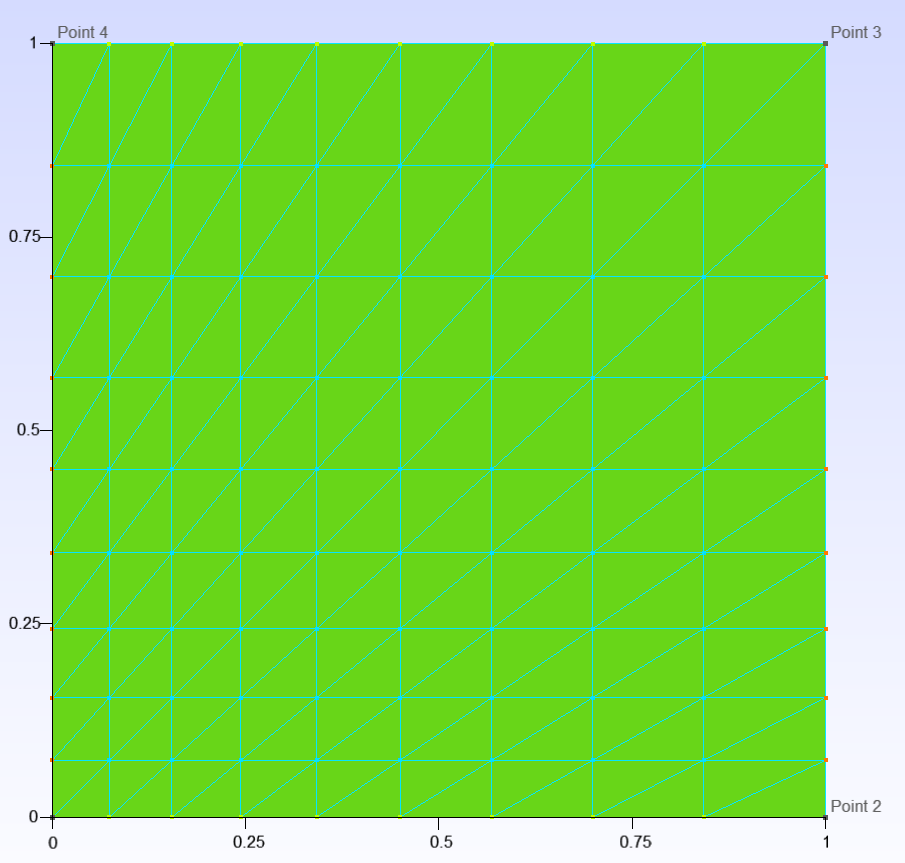
\includegraphics[width=\textwidth]{CST_mesh.png}
        \caption{Mesh using CST elements.}
        \label{fig:cst_mesh}
    \end{subfigure}
    \hfill
    \begin{subfigure}[t]{0.45\textwidth}
        \centering
        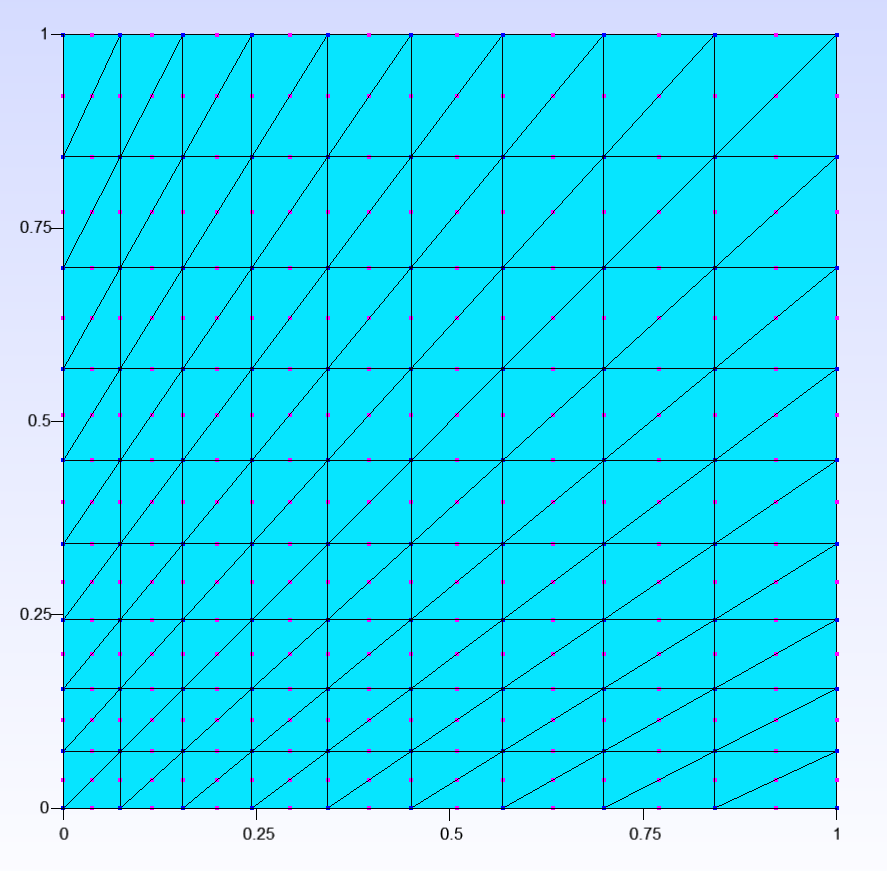
\includegraphics[width=\textwidth]{LST_mesh.png}
        \caption{Mesh using LST elements.}
        \label{fig:lst_mesh}
    \end{subfigure}
    \caption{Comparison of the mesh for CST and LST finite elements.}
    \label{fig:mesh_comparison}
\end{figure}

\subsection{CST Elements}

\begin{figure}[H]
    \centering
    \begin{subfigure}[t]{0.32\textwidth}
        \centering
        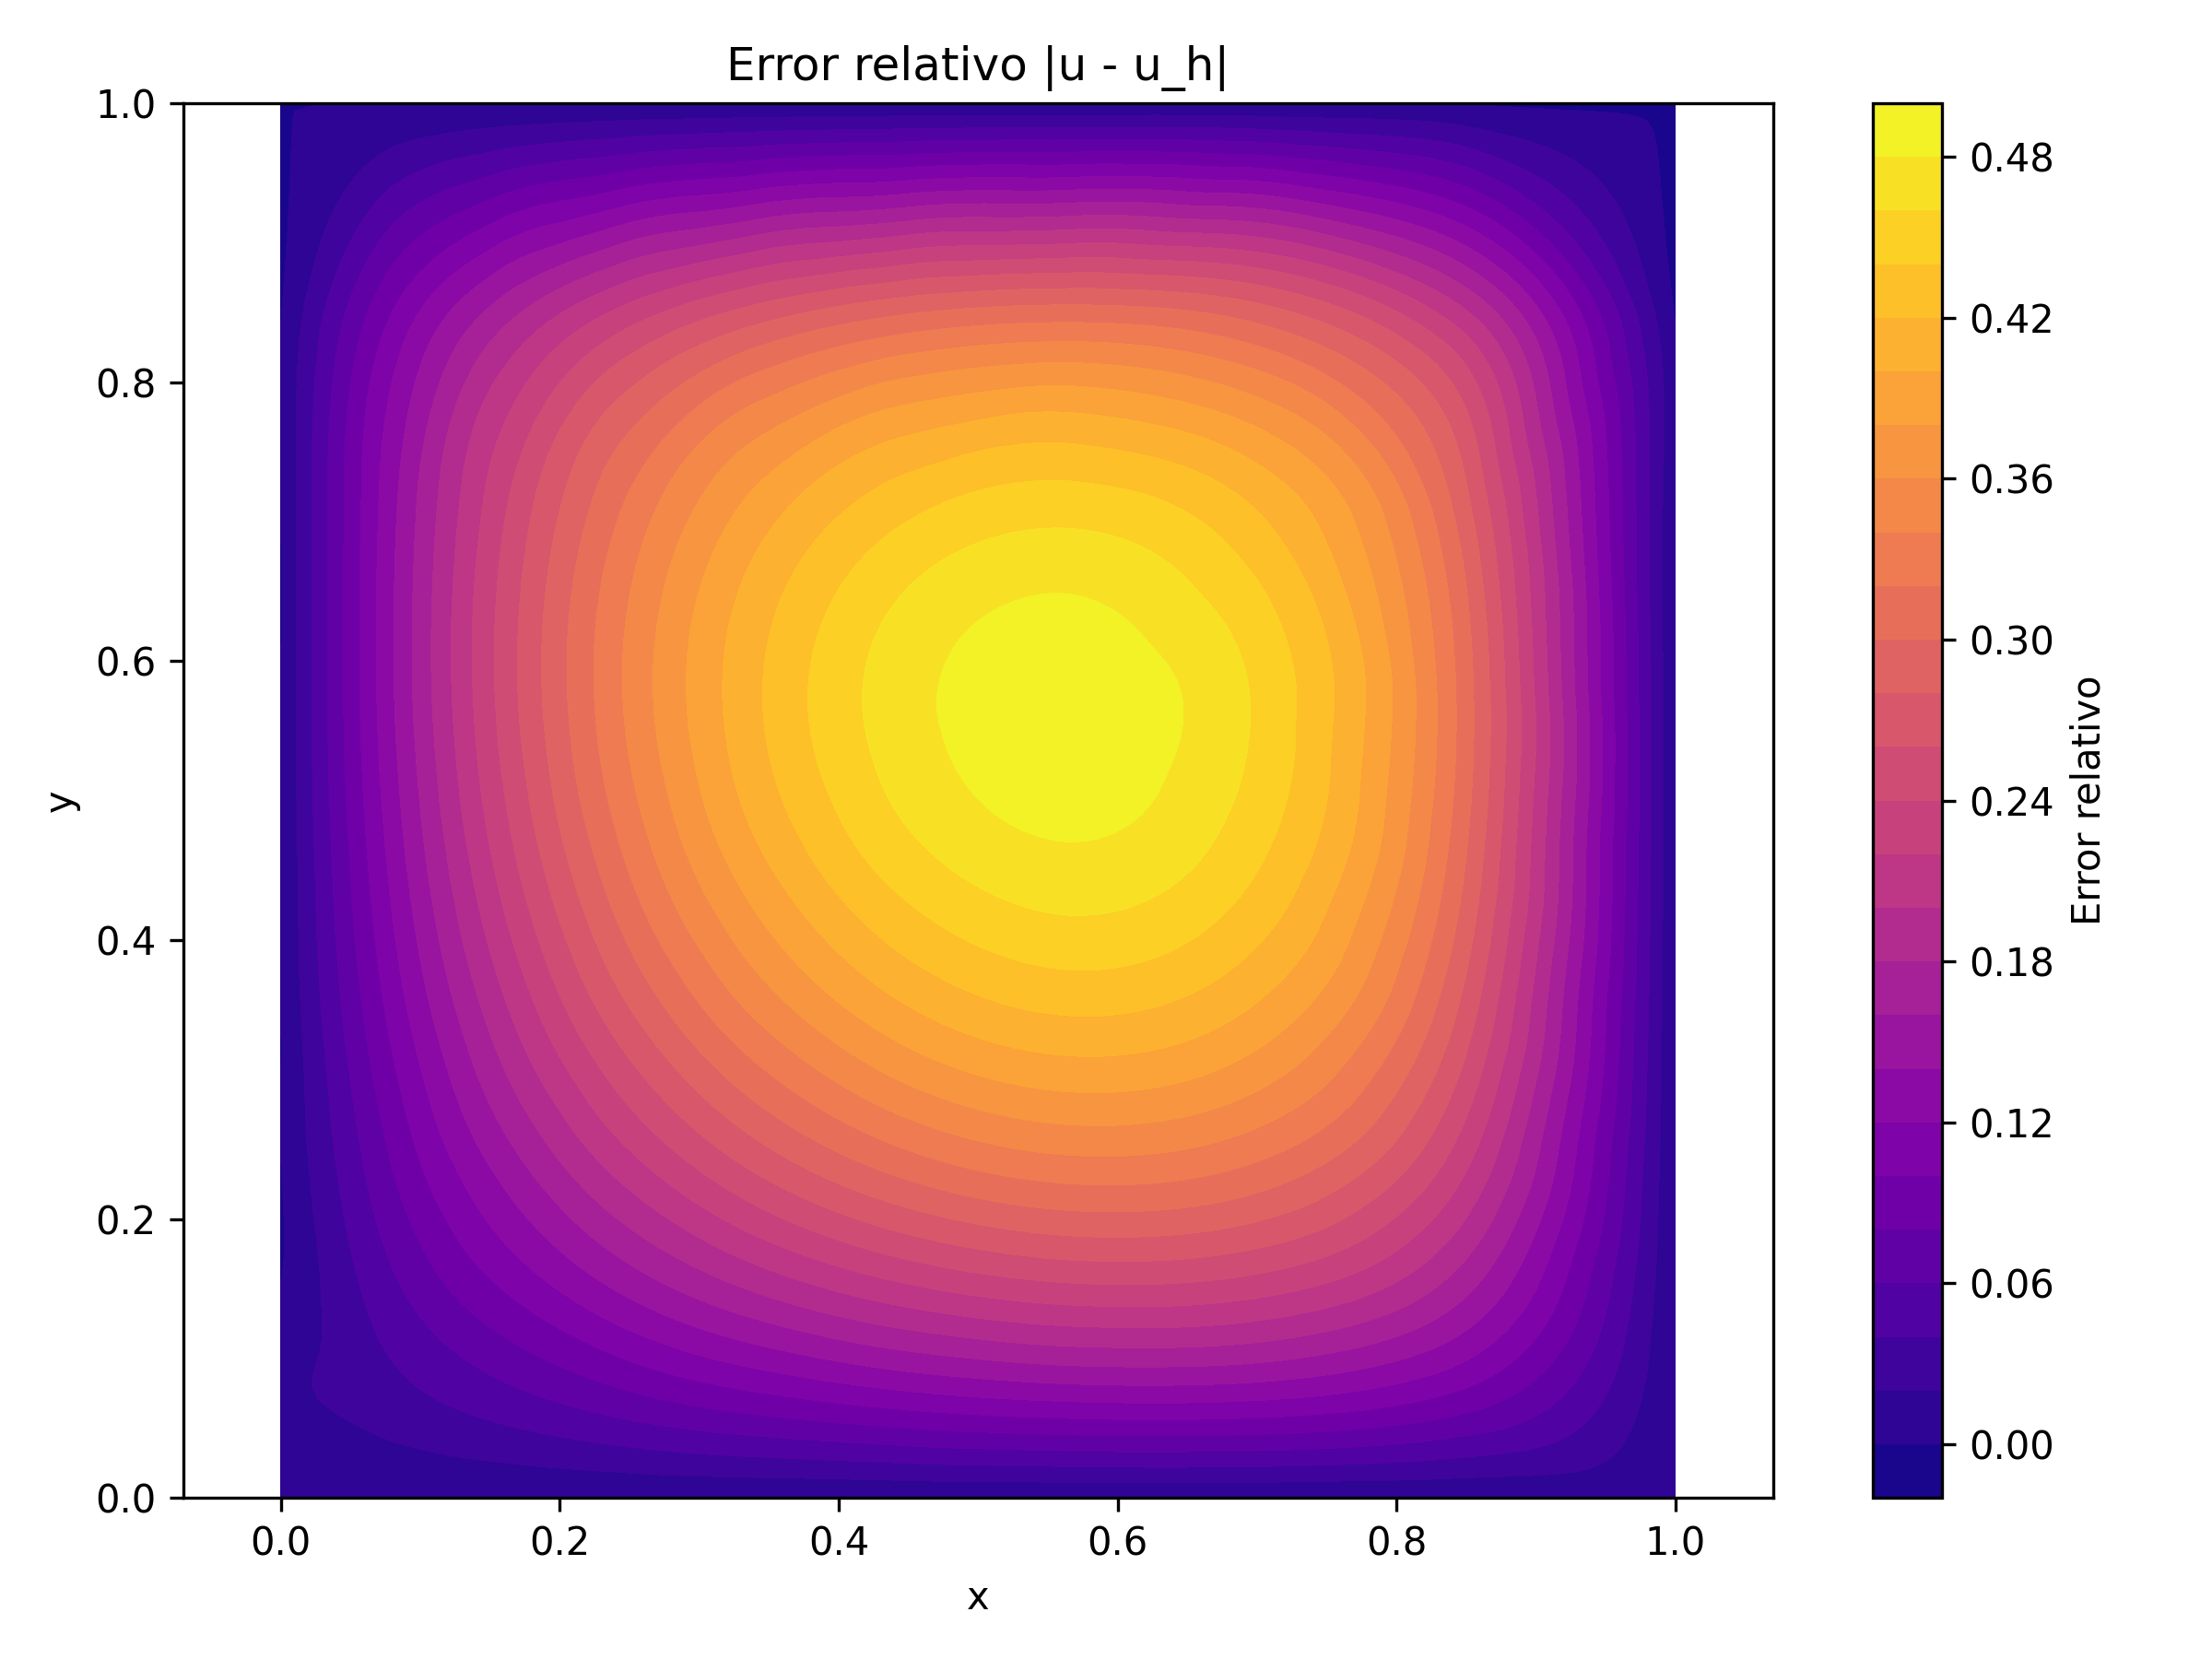
\includegraphics[width=\textwidth]{Graficos/11/CST_relative_error_colormap.png}
        \caption{CST error (N = 10, r = 1.1)}
        \label{fig:cst_error_r1.1}
    \end{subfigure}
    \hfill
    \begin{subfigure}[t]{0.32\textwidth}
        \centering
        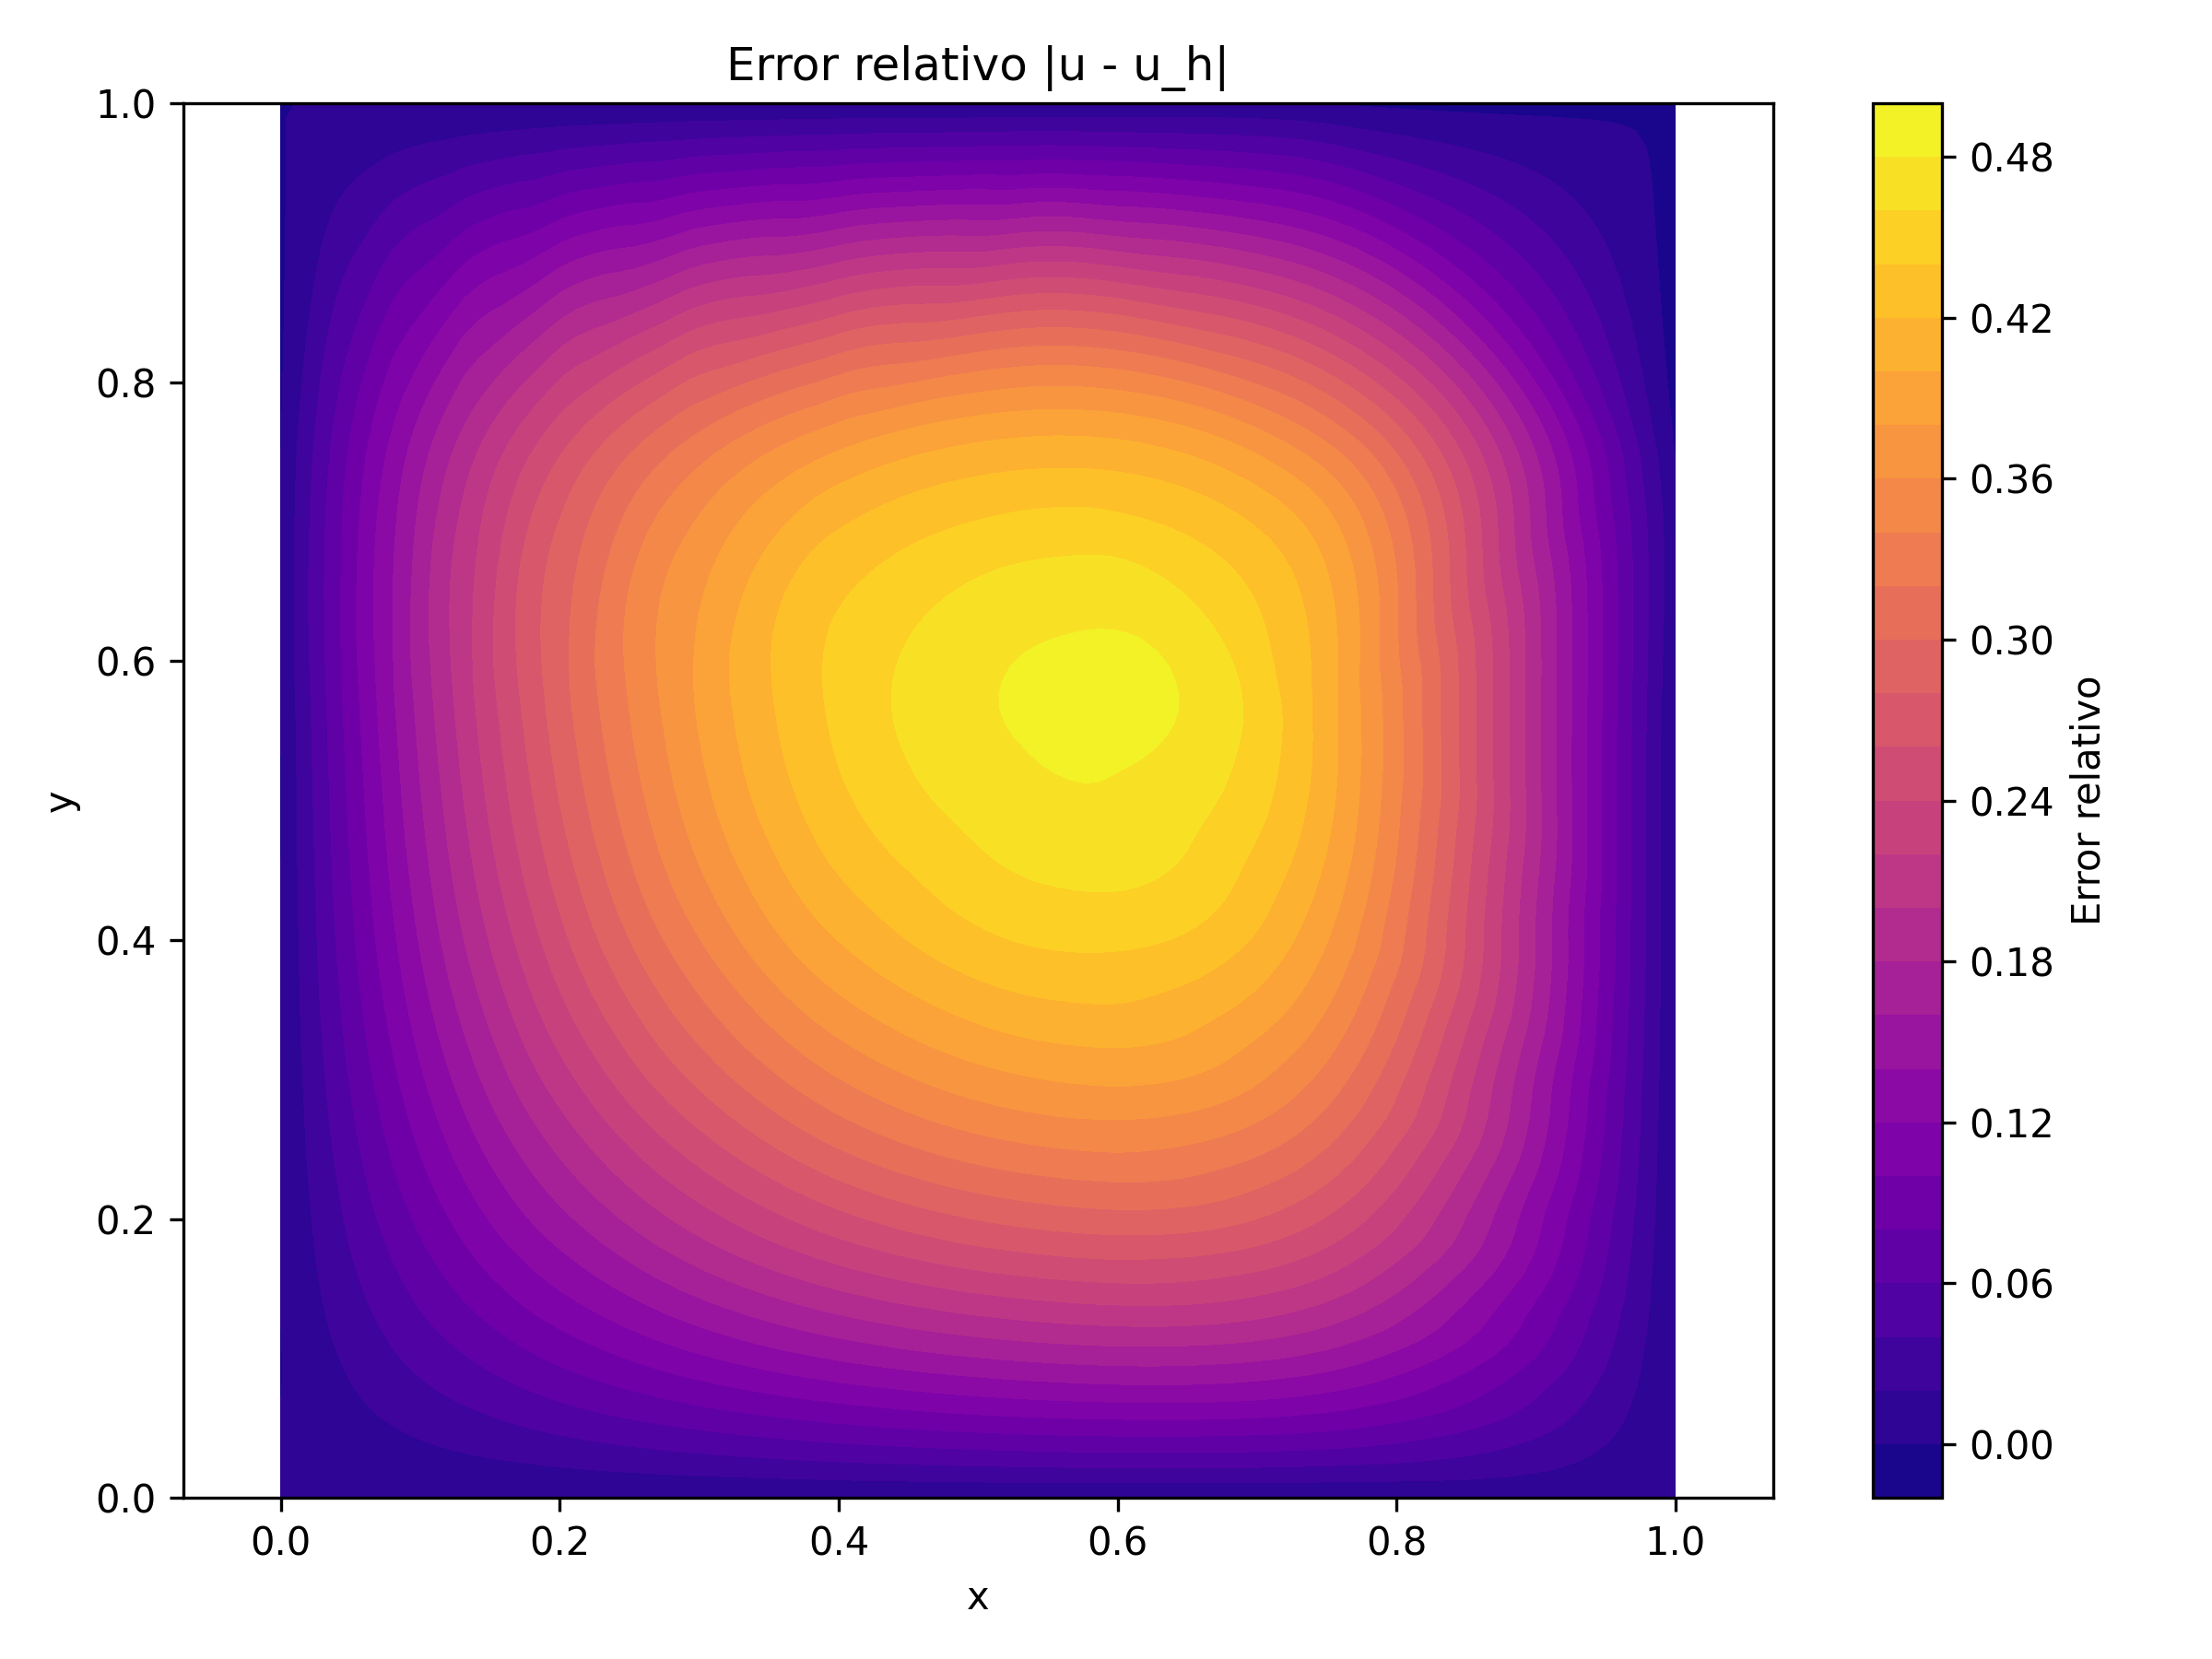
\includegraphics[width=\textwidth]{Graficos/12/CST_relative_error_colormap.png}
        \caption{CST error (N = 10, r = 1.2)}
        \label{fig:cst_error_r1.2}
    \end{subfigure}
    \hfill
    \begin{subfigure}[t]{0.32\textwidth}
        \centering
        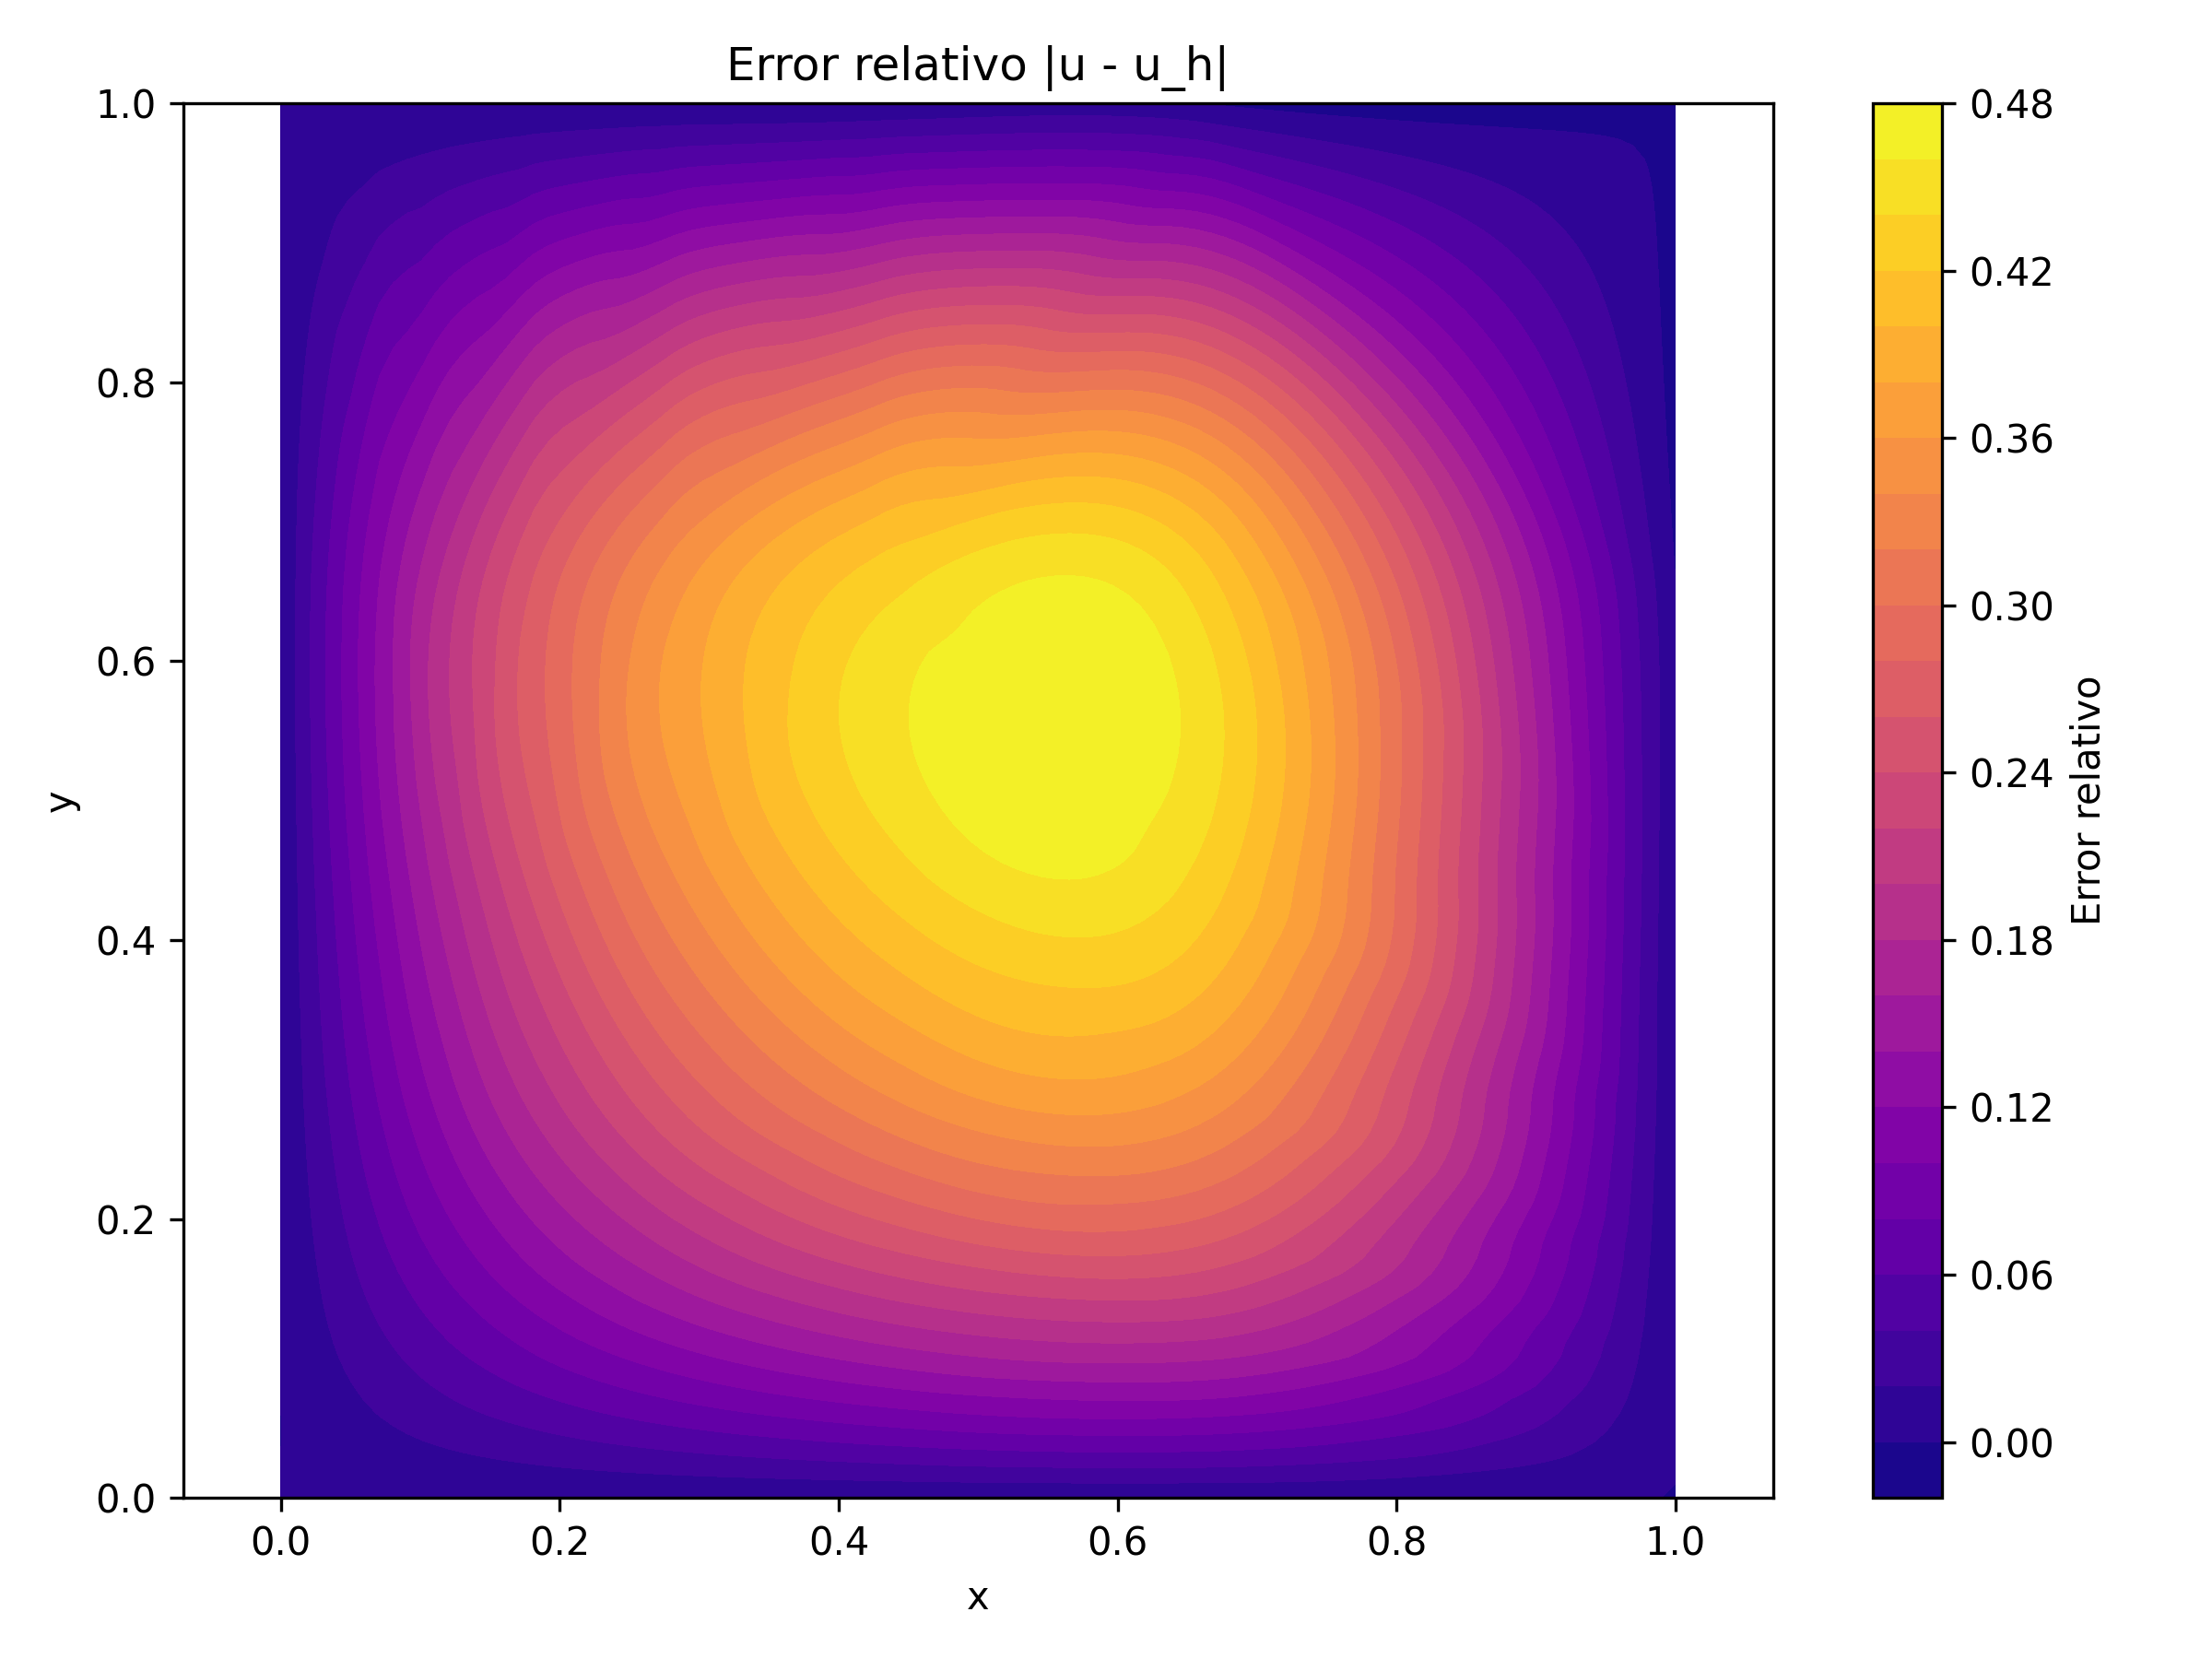
\includegraphics[width=\textwidth]{Graficos/13/CST_relative_error_colormap.png}
        \caption{CST error (N = 10, r = 1.3)}
        \label{fig:cst_error_r1.3}
    \end{subfigure}
    \caption{Relative error for CST elements with $N = 10$ and different values of $r$.}
    \label{fig:cst_error_comparison}
\end{figure}

\begin{figure}[H]
    \centering
    \begin{subfigure}[t]{0.32\textwidth}
        \centering
        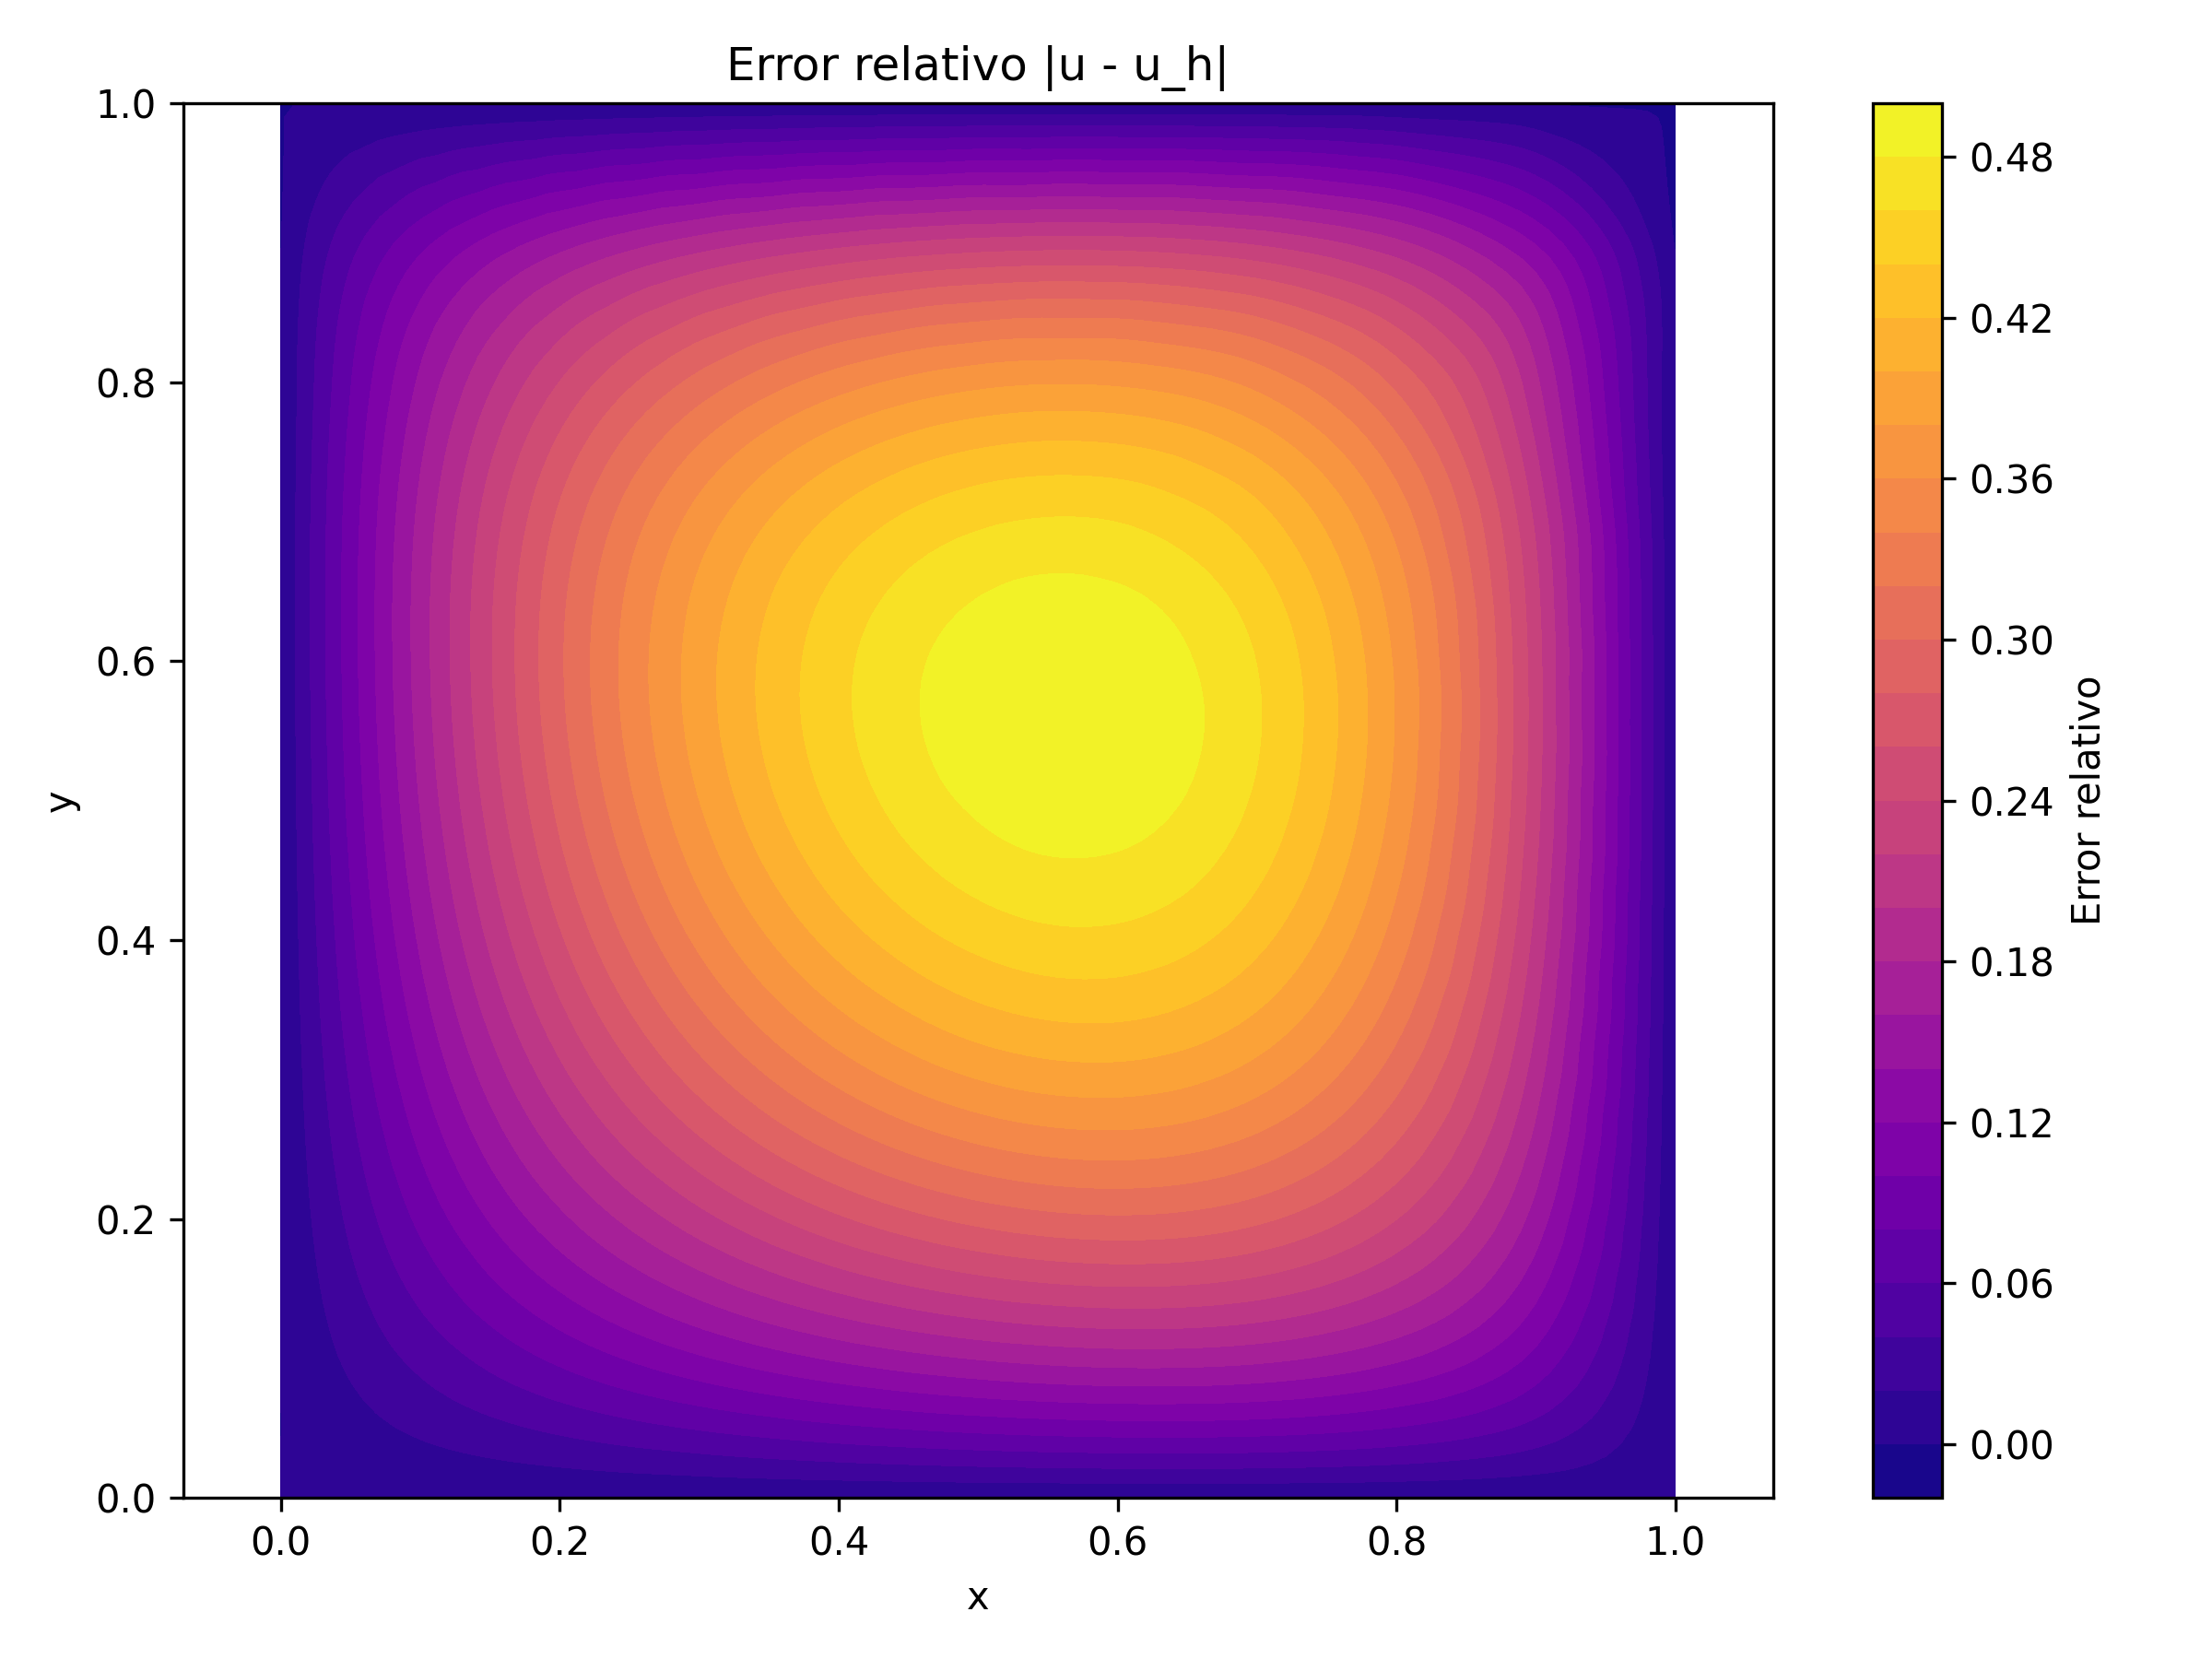
\includegraphics[width=\textwidth]{Graficos/21/CST_relative_error_colormap.png}
        \caption{CST error (N = 20, r = 1.1)}
        \label{fig:cst_error_r1.1_n20}
    \end{subfigure}
    \hfill
    \begin{subfigure}[t]{0.32\textwidth}
        \centering
        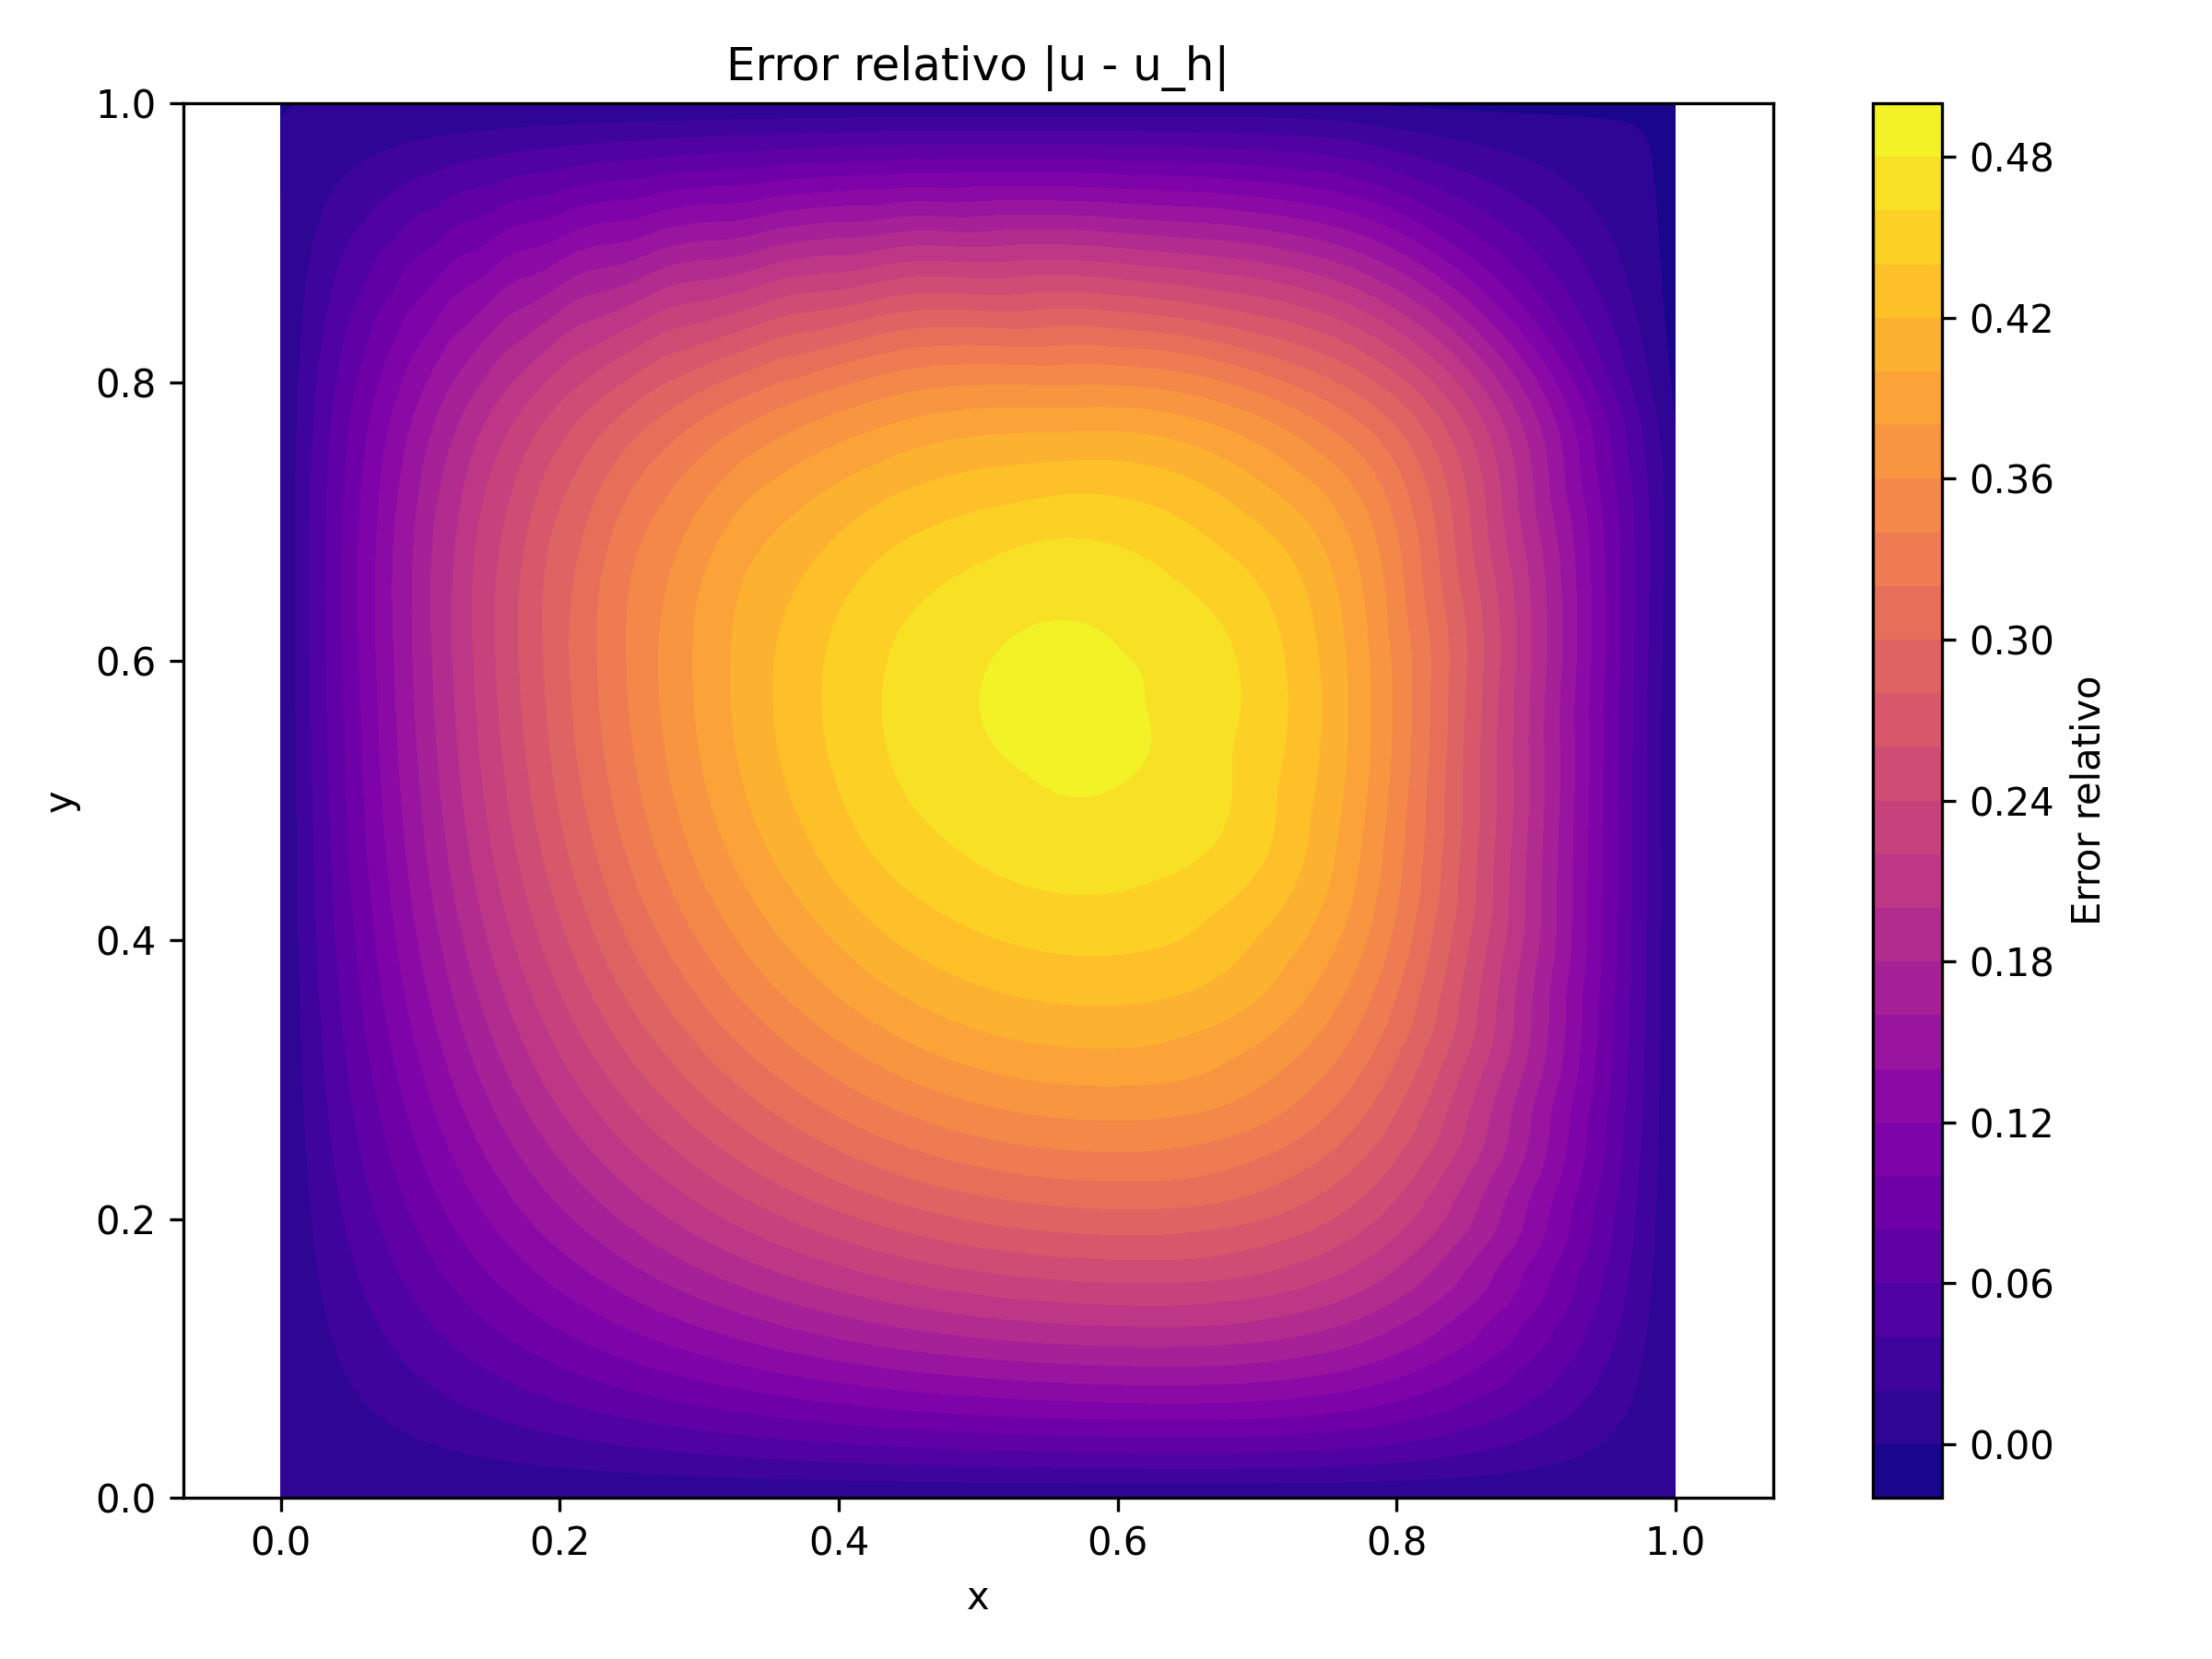
\includegraphics[width=\textwidth]{Graficos/22/CST_relative_error_colormap.png}
        \caption{CST error (N = 20, r = 1.2)}
        \label{fig:cst_error_r1.2_n20}
    \end{subfigure}
    \hfill
    \begin{subfigure}[t]{0.32\textwidth}
        \centering
        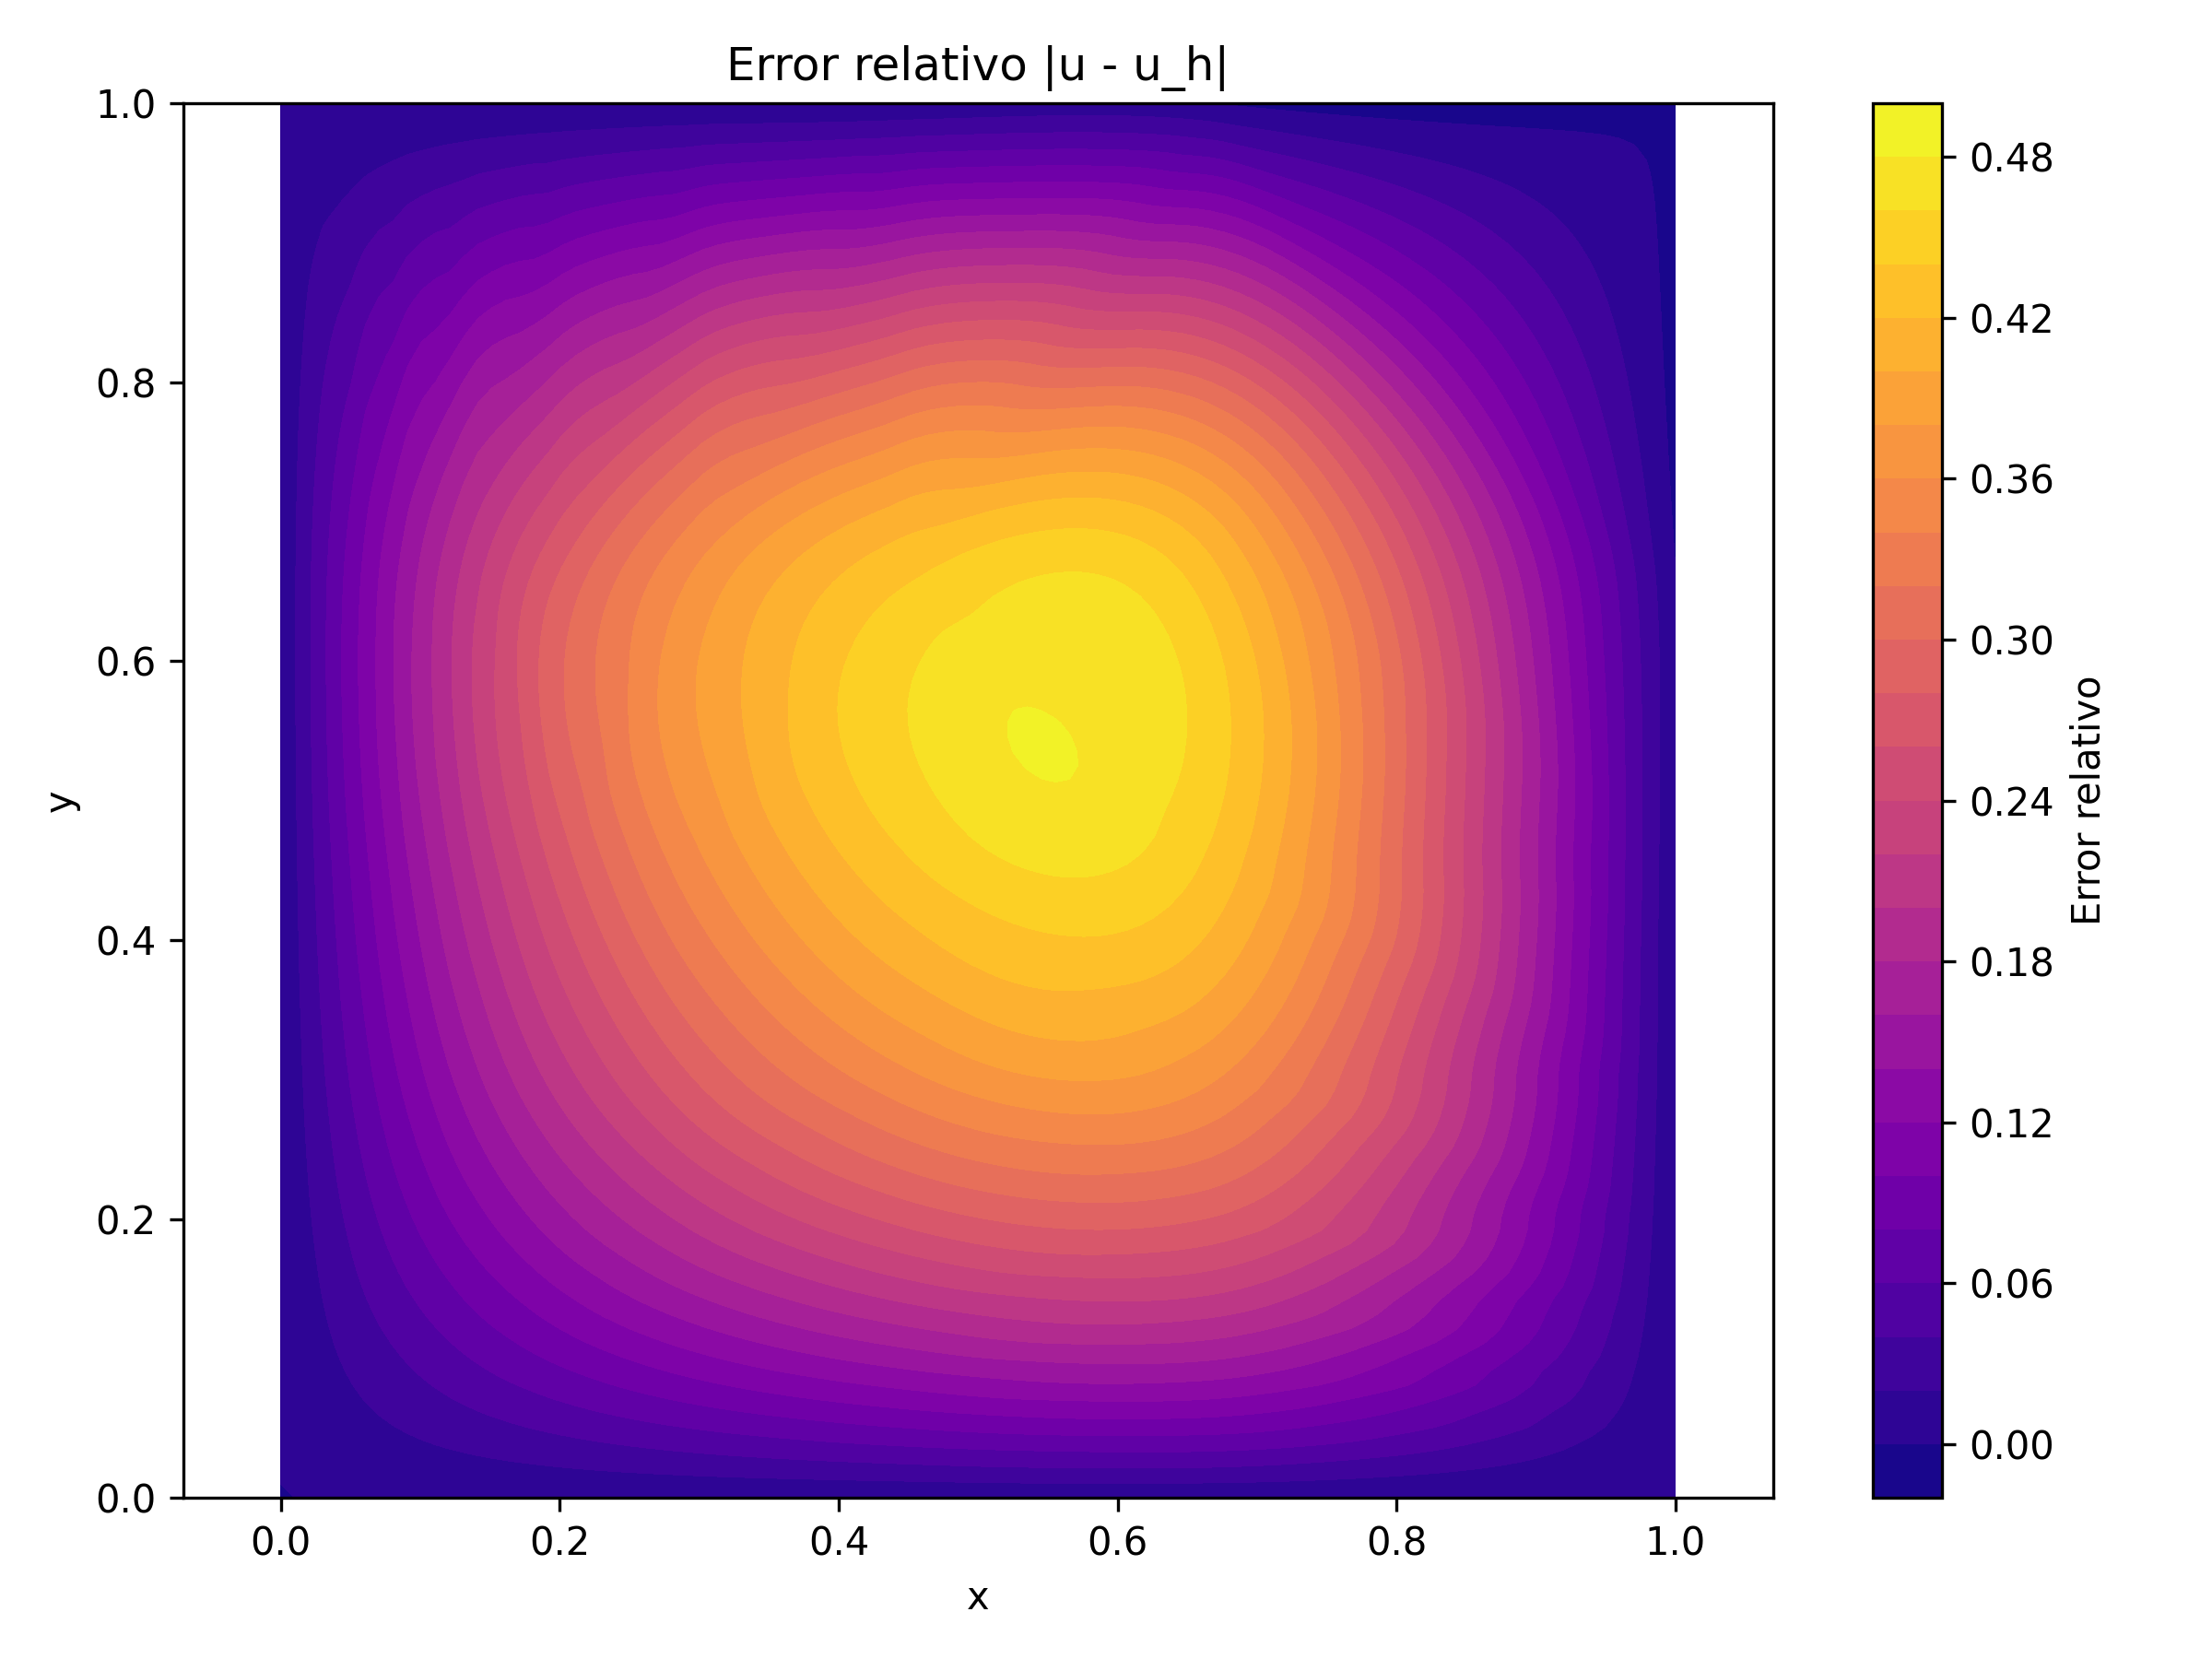
\includegraphics[width=\textwidth]{Graficos/23/CST_relative_error_colormap.png}
        \caption{CST error (N = 20, r = 1.3)}
        \label{fig:cst_error_r1.3_n20}
    \end{subfigure}
    \caption{Relative error for CST elements with $N = 20$ and different values of $r$.}
    \label{fig:cst_error_comparison_n20}
\end{figure}


\begin{figure}[H]
    \centering
    \begin{subfigure}[t]{0.32\textwidth}
        \centering
        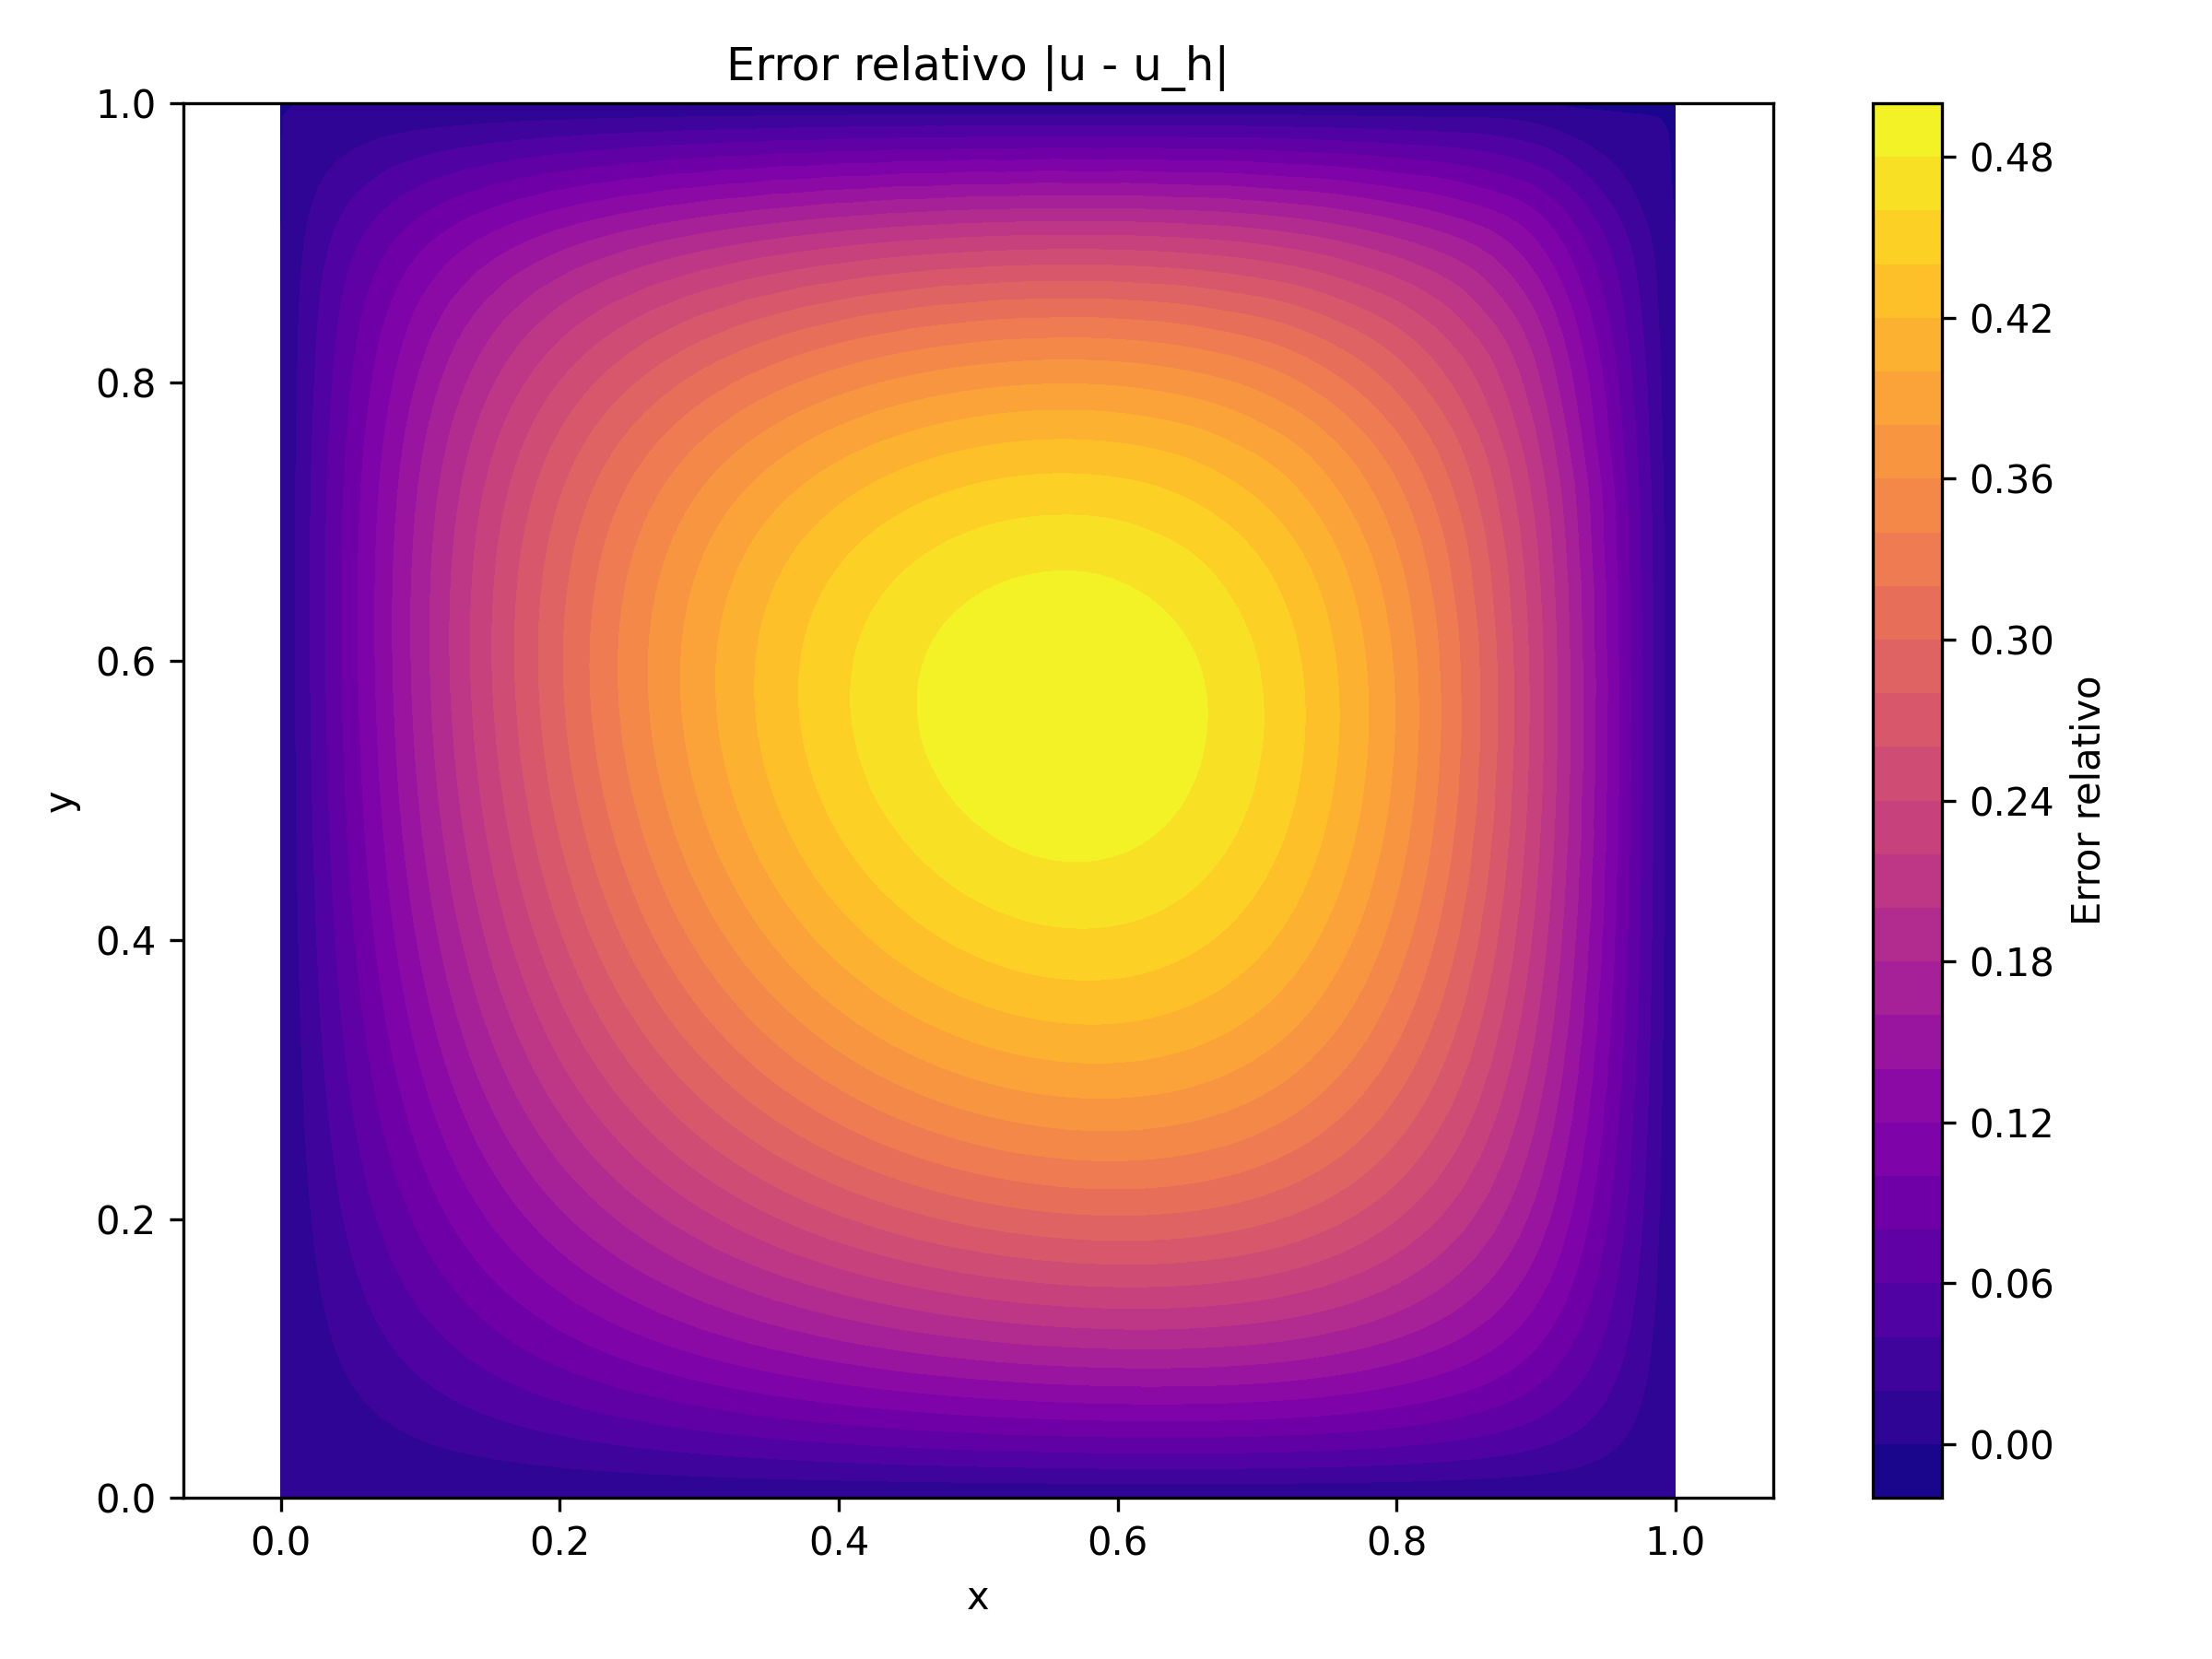
\includegraphics[width=\textwidth]{Graficos/31/CST_relative_error_colormap.png}
        \caption{CST error (N = 30, r = 1.1)}
        \label{fig:cst_error_r1.1_n30}
    \end{subfigure}
    \hfill
    \begin{subfigure}[t]{0.32\textwidth}
        \centering
        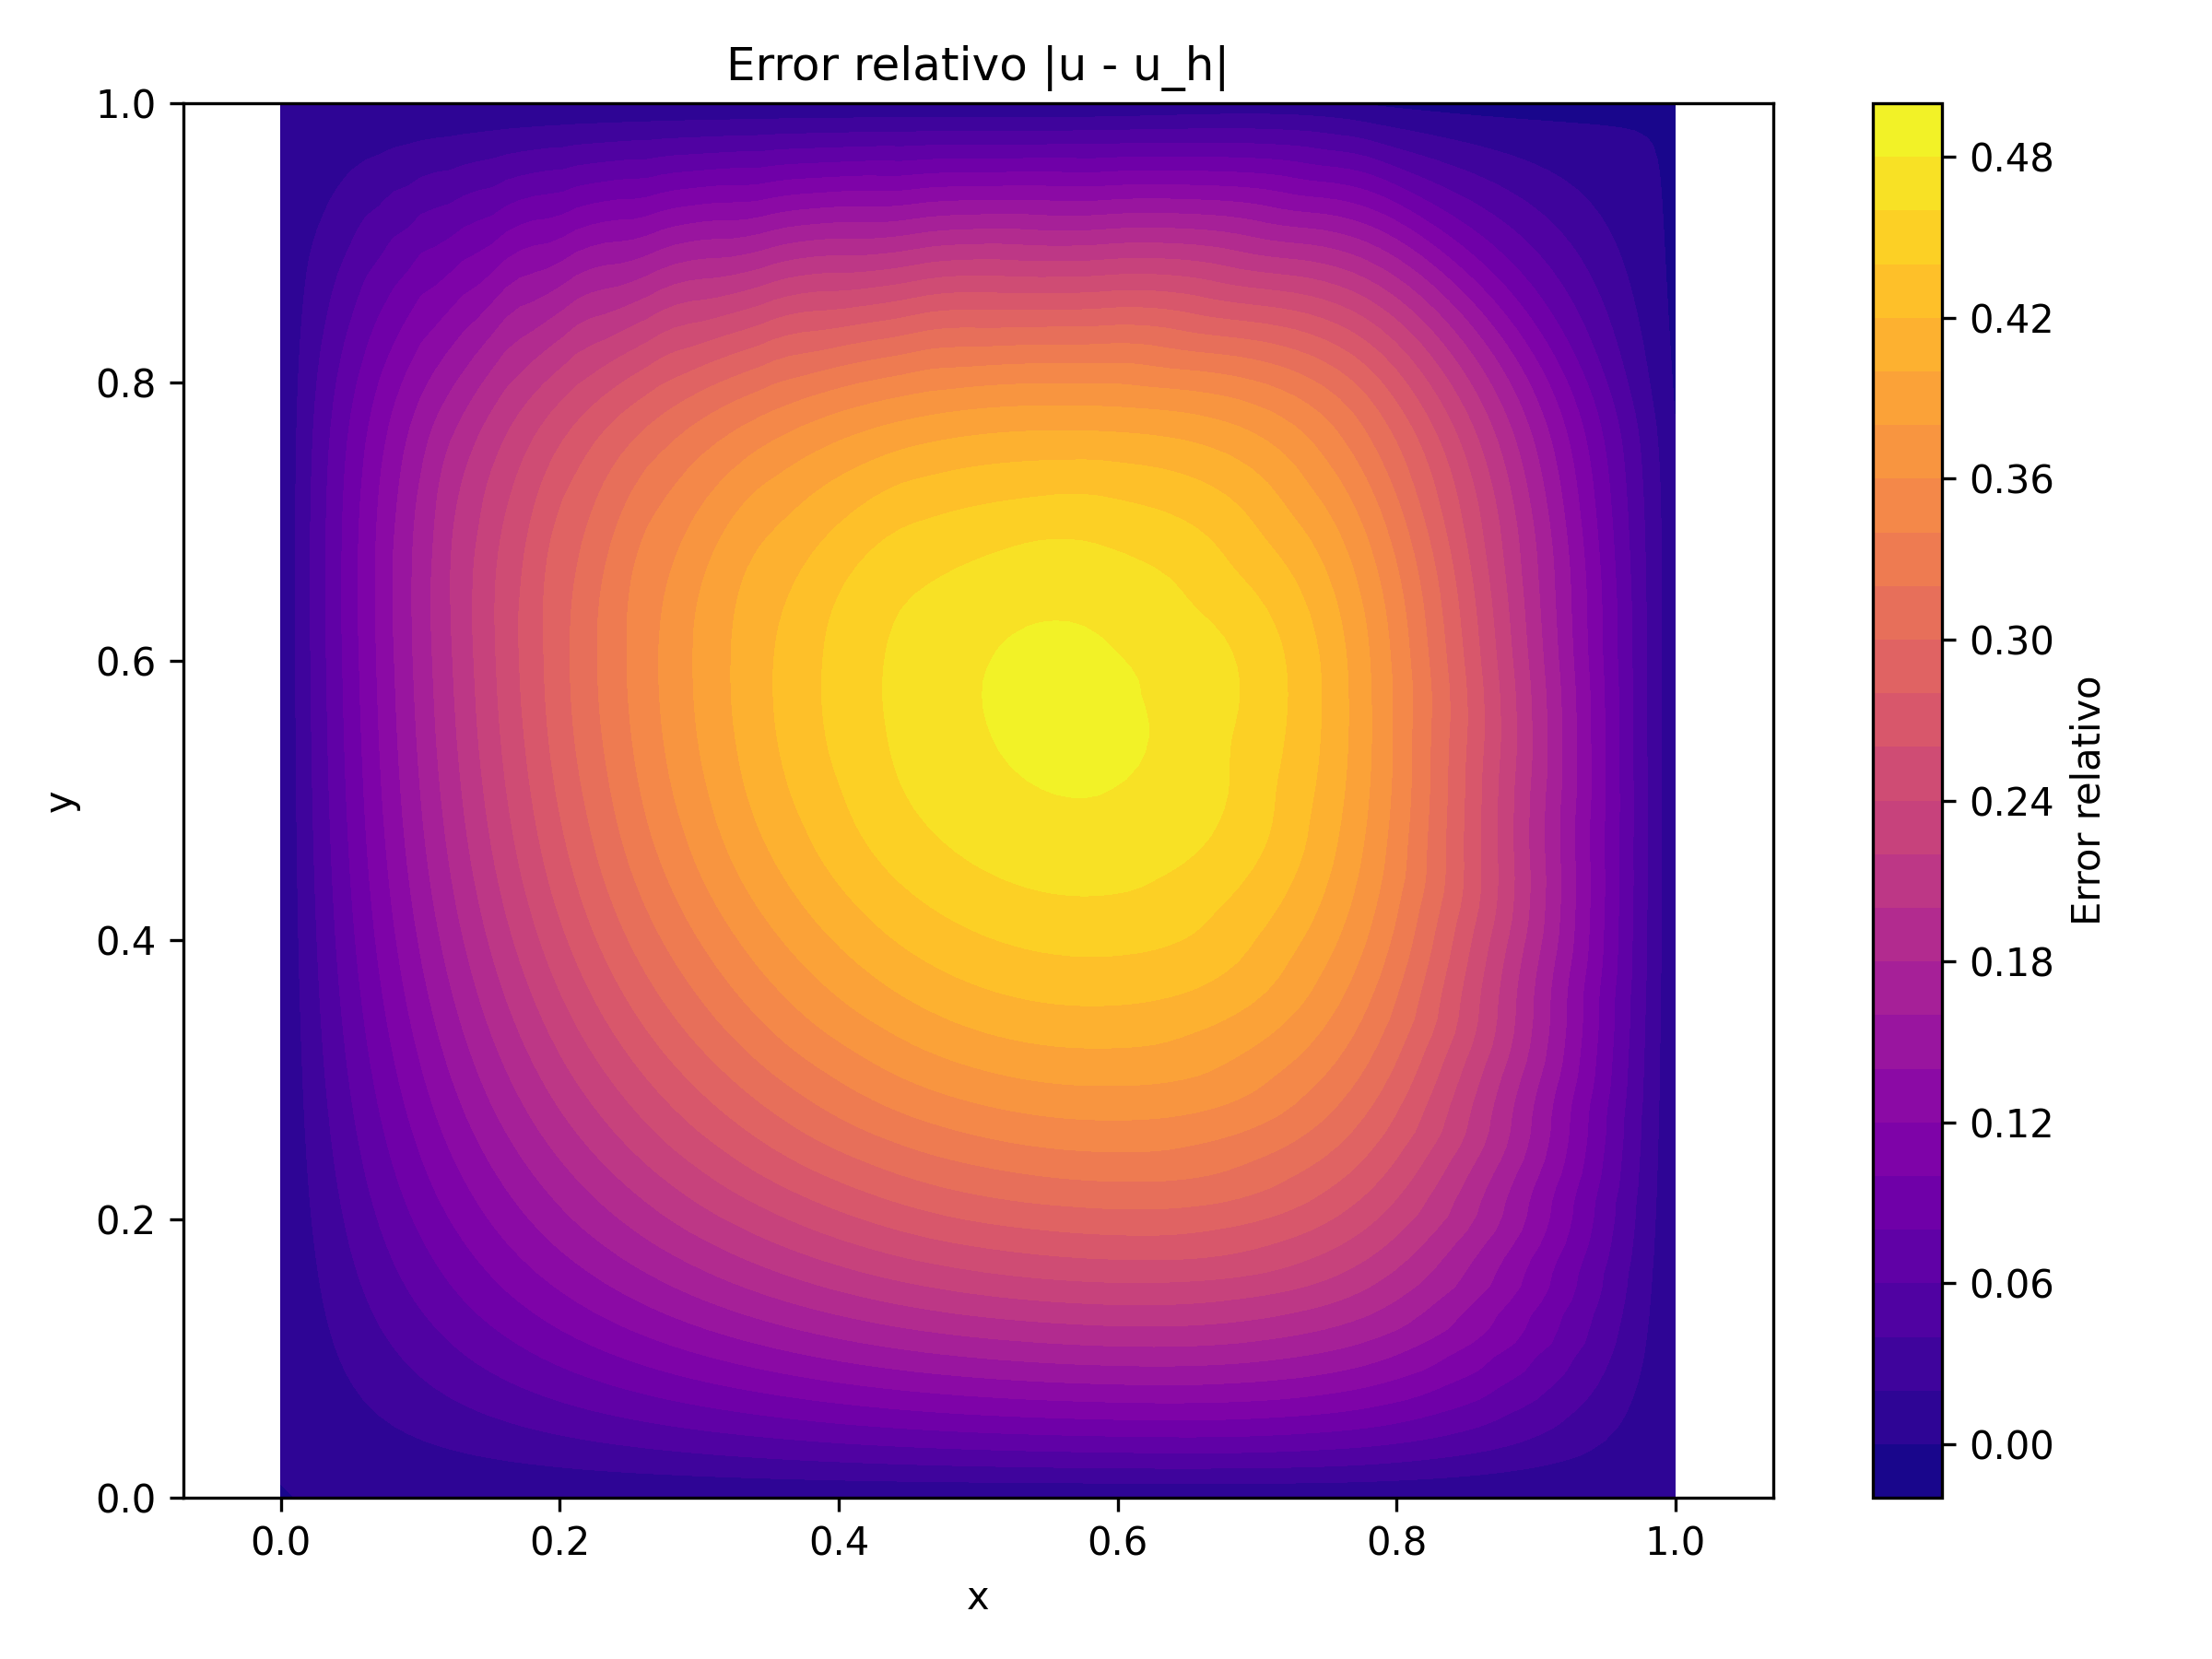
\includegraphics[width=\textwidth]{Graficos/32/CST_relative_error_colormap.png}
        \caption{CST error (N = 30, r = 1.2)}
        \label{fig:cst_error_r1.2_n30}
    \end{subfigure}
    \hfill
    \begin{subfigure}[t]{0.32\textwidth}
        \centering
        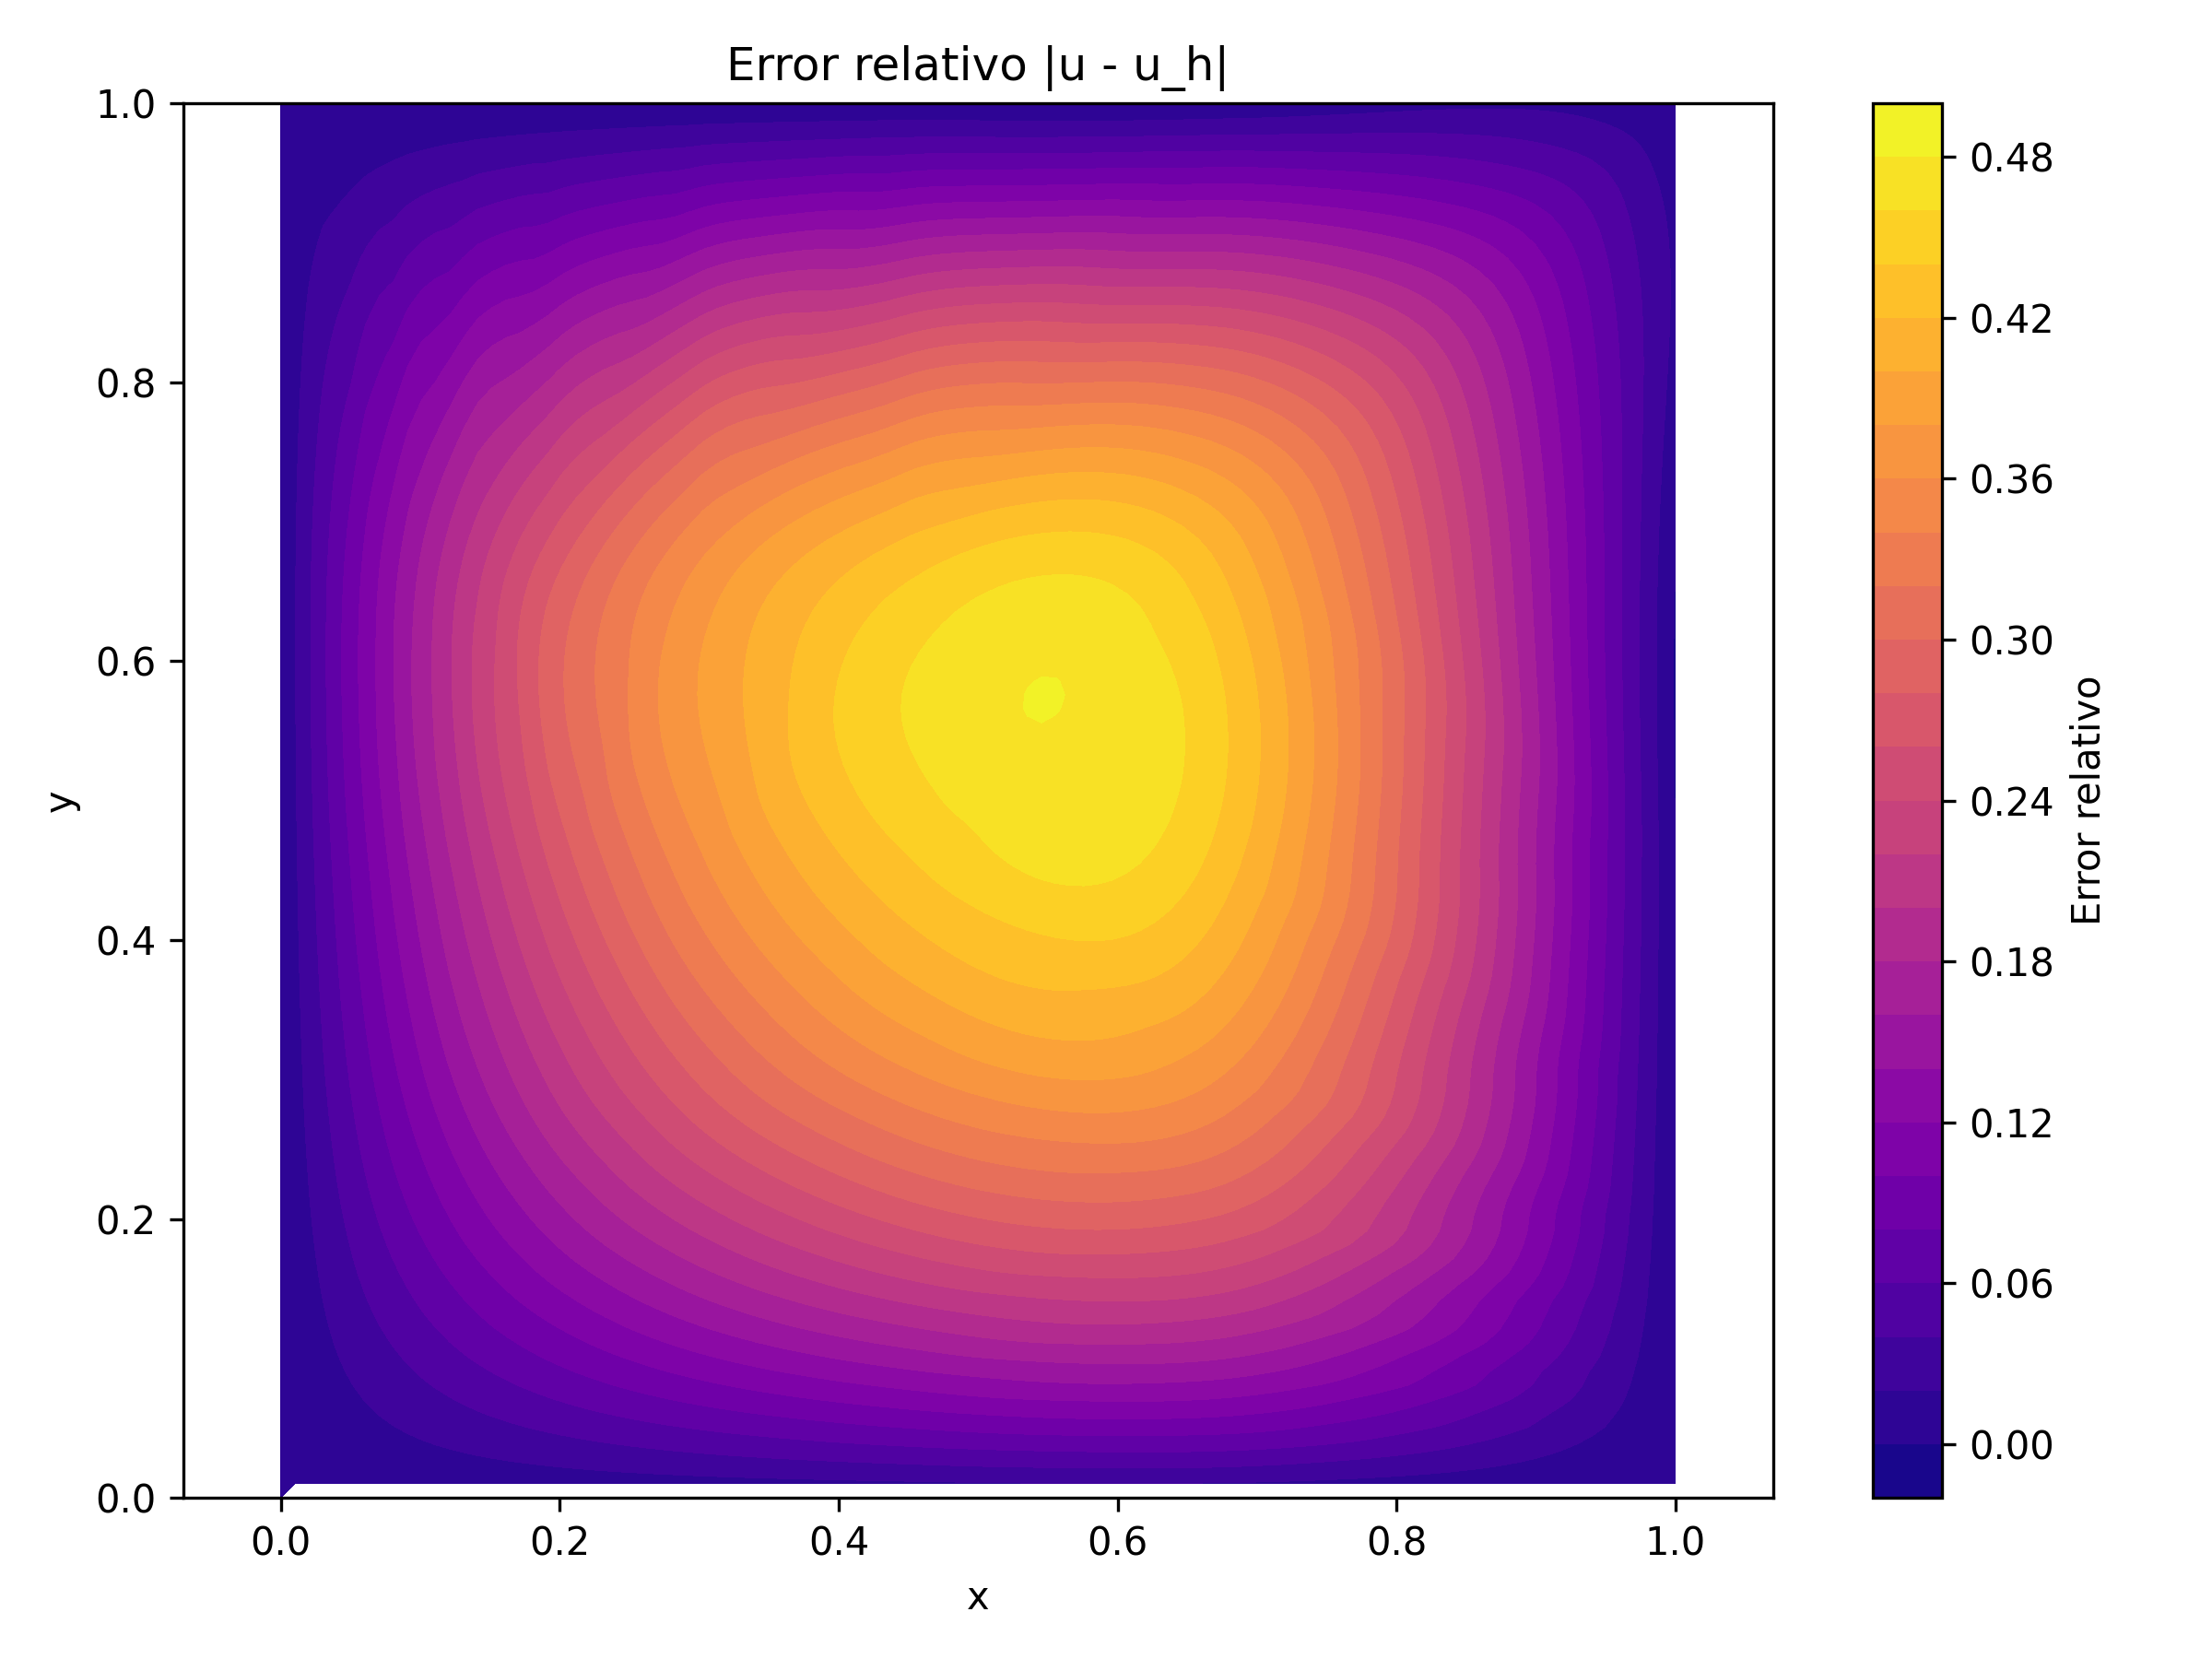
\includegraphics[width=\textwidth]{Graficos/33/CST_relative_error_colormap.png}
        \caption{CST error (N = 30, r = 1.3)}
        \label{fig:cst_error_r1.3_n30}
    \end{subfigure}
    \caption{Relative error for CST elements with $N = 30$ and different values of $r$.}
    \label{fig:cst_error_comparison_n30}
\end{figure}

The relative error in CST elements tends to concentrate in regions that are far from the boundary conditions and from the smaller elements of the mesh. This happens because, lacking intermediate nodes, CST elements have limited capacity to capture variations in the displacement field. As the distance increases from well-conditioned or refined zones, the accuracy of the linear interpolation deteriorates and the error increases. This can be observed in the relative error figures for CST, where the error remains higher near the corner with the largest elements (specifically, the upper right corner of our mesh).


\subsection{LST Elements}

\begin{figure}[H]
    \centering
    \begin{subfigure}[t]{0.32\textwidth}
        \centering
        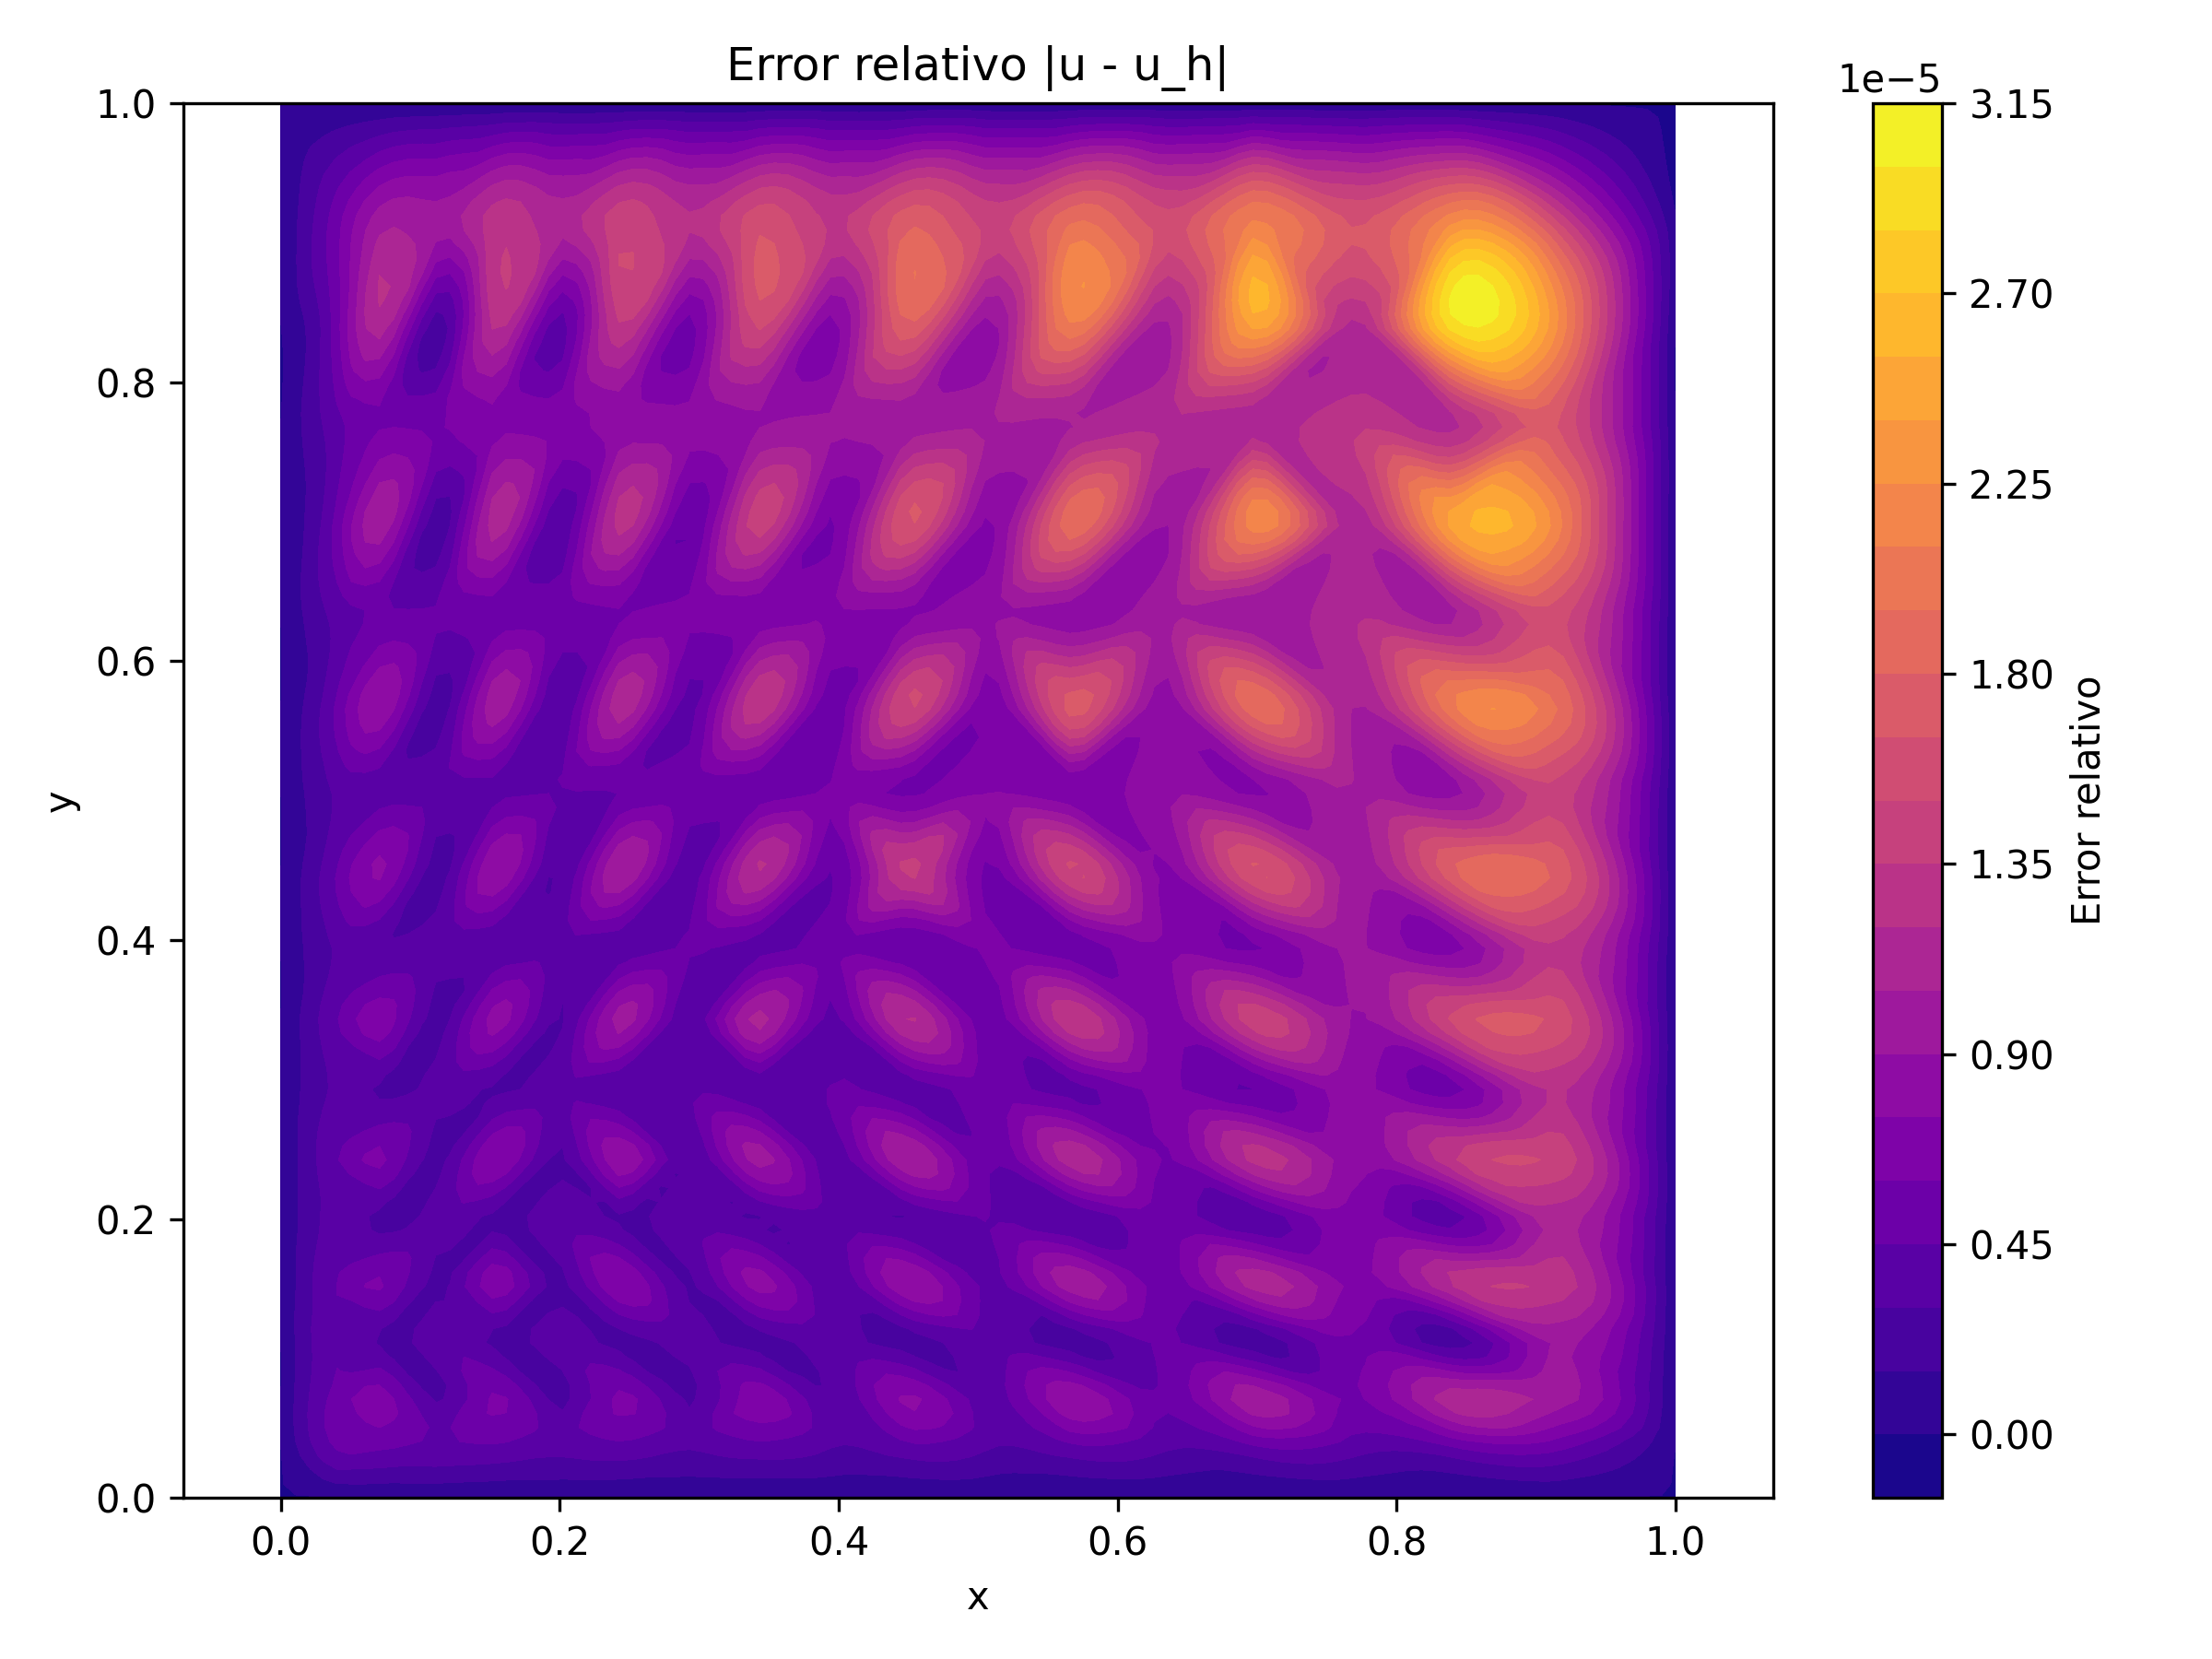
\includegraphics[width=\textwidth]{Graficos/11/LST_relative_error_colormap.png}
        \caption{LST error (N = 10, r = 1.1)}
        \label{fig:lst_error_r1.1}
    \end{subfigure}
    \hfill
    \begin{subfigure}[t]{0.32\textwidth}
        \centering
        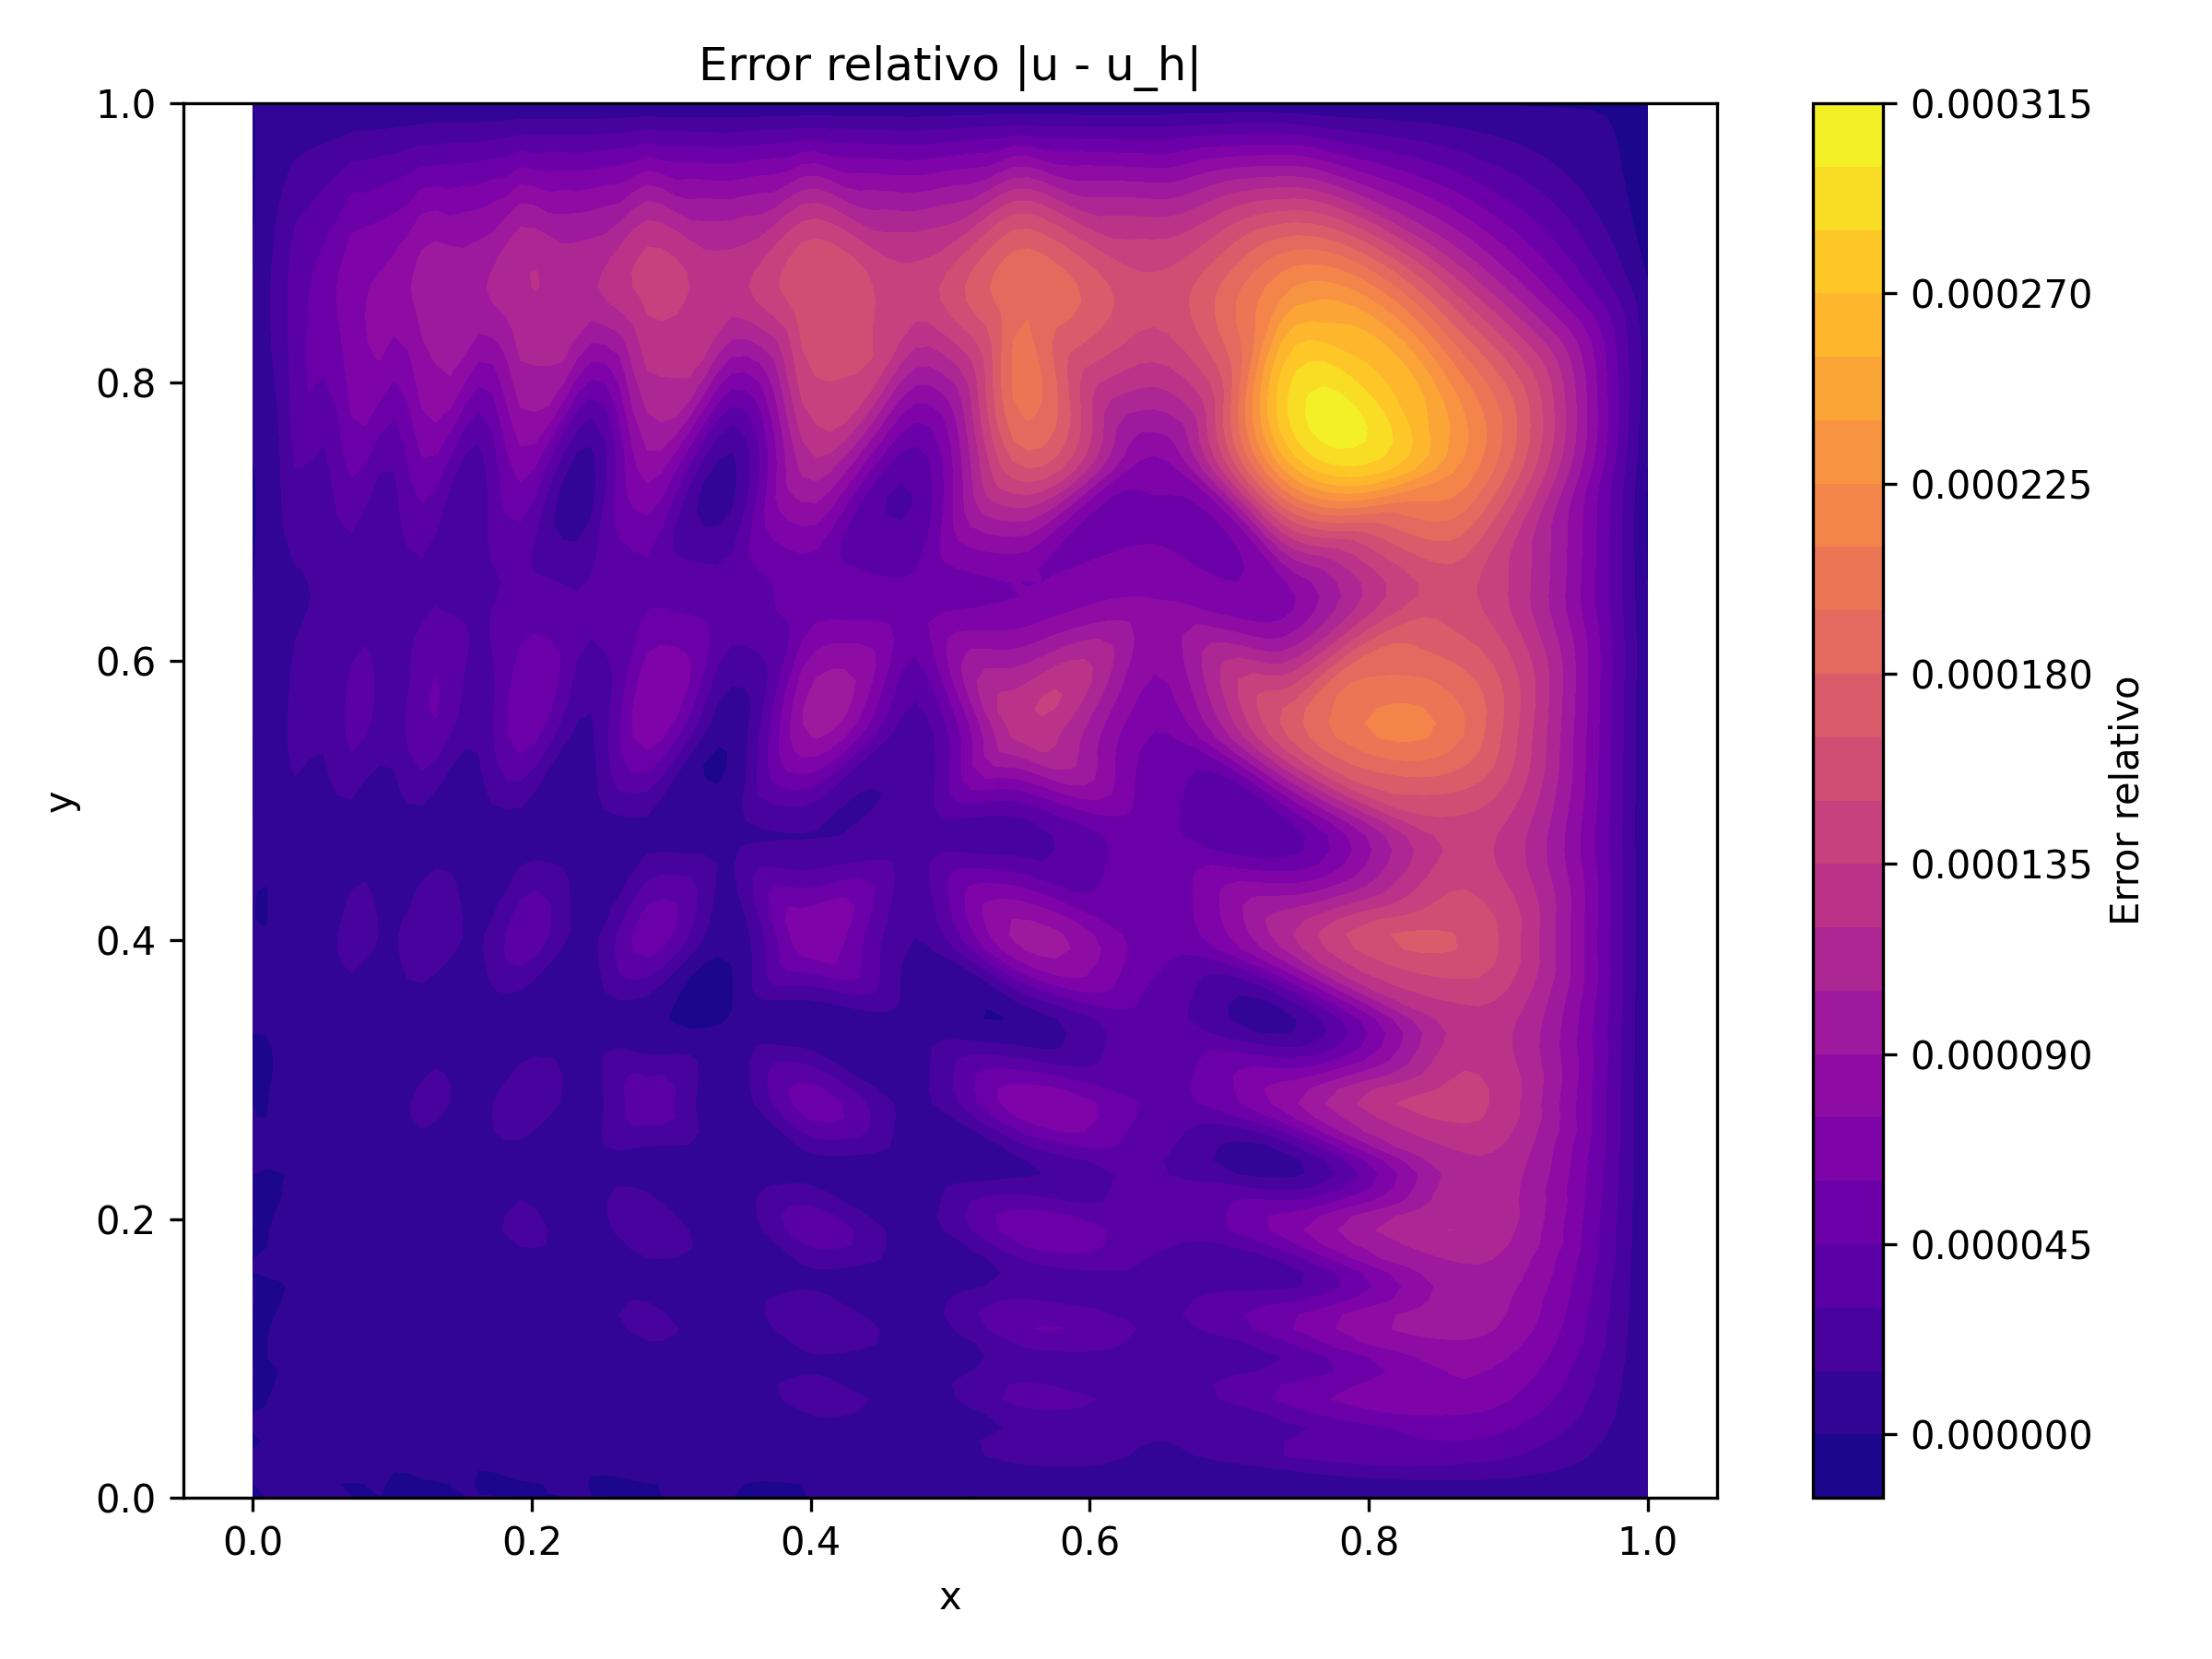
\includegraphics[width=\textwidth]{Graficos/12/LST_relative_error_colormap.png}
        \caption{LST error (N = 10, r = 1.2)}
        \label{fig:lst_error_r1.2}
    \end{subfigure}
    \hfill
    \begin{subfigure}[t]{0.32\textwidth}
        \centering
        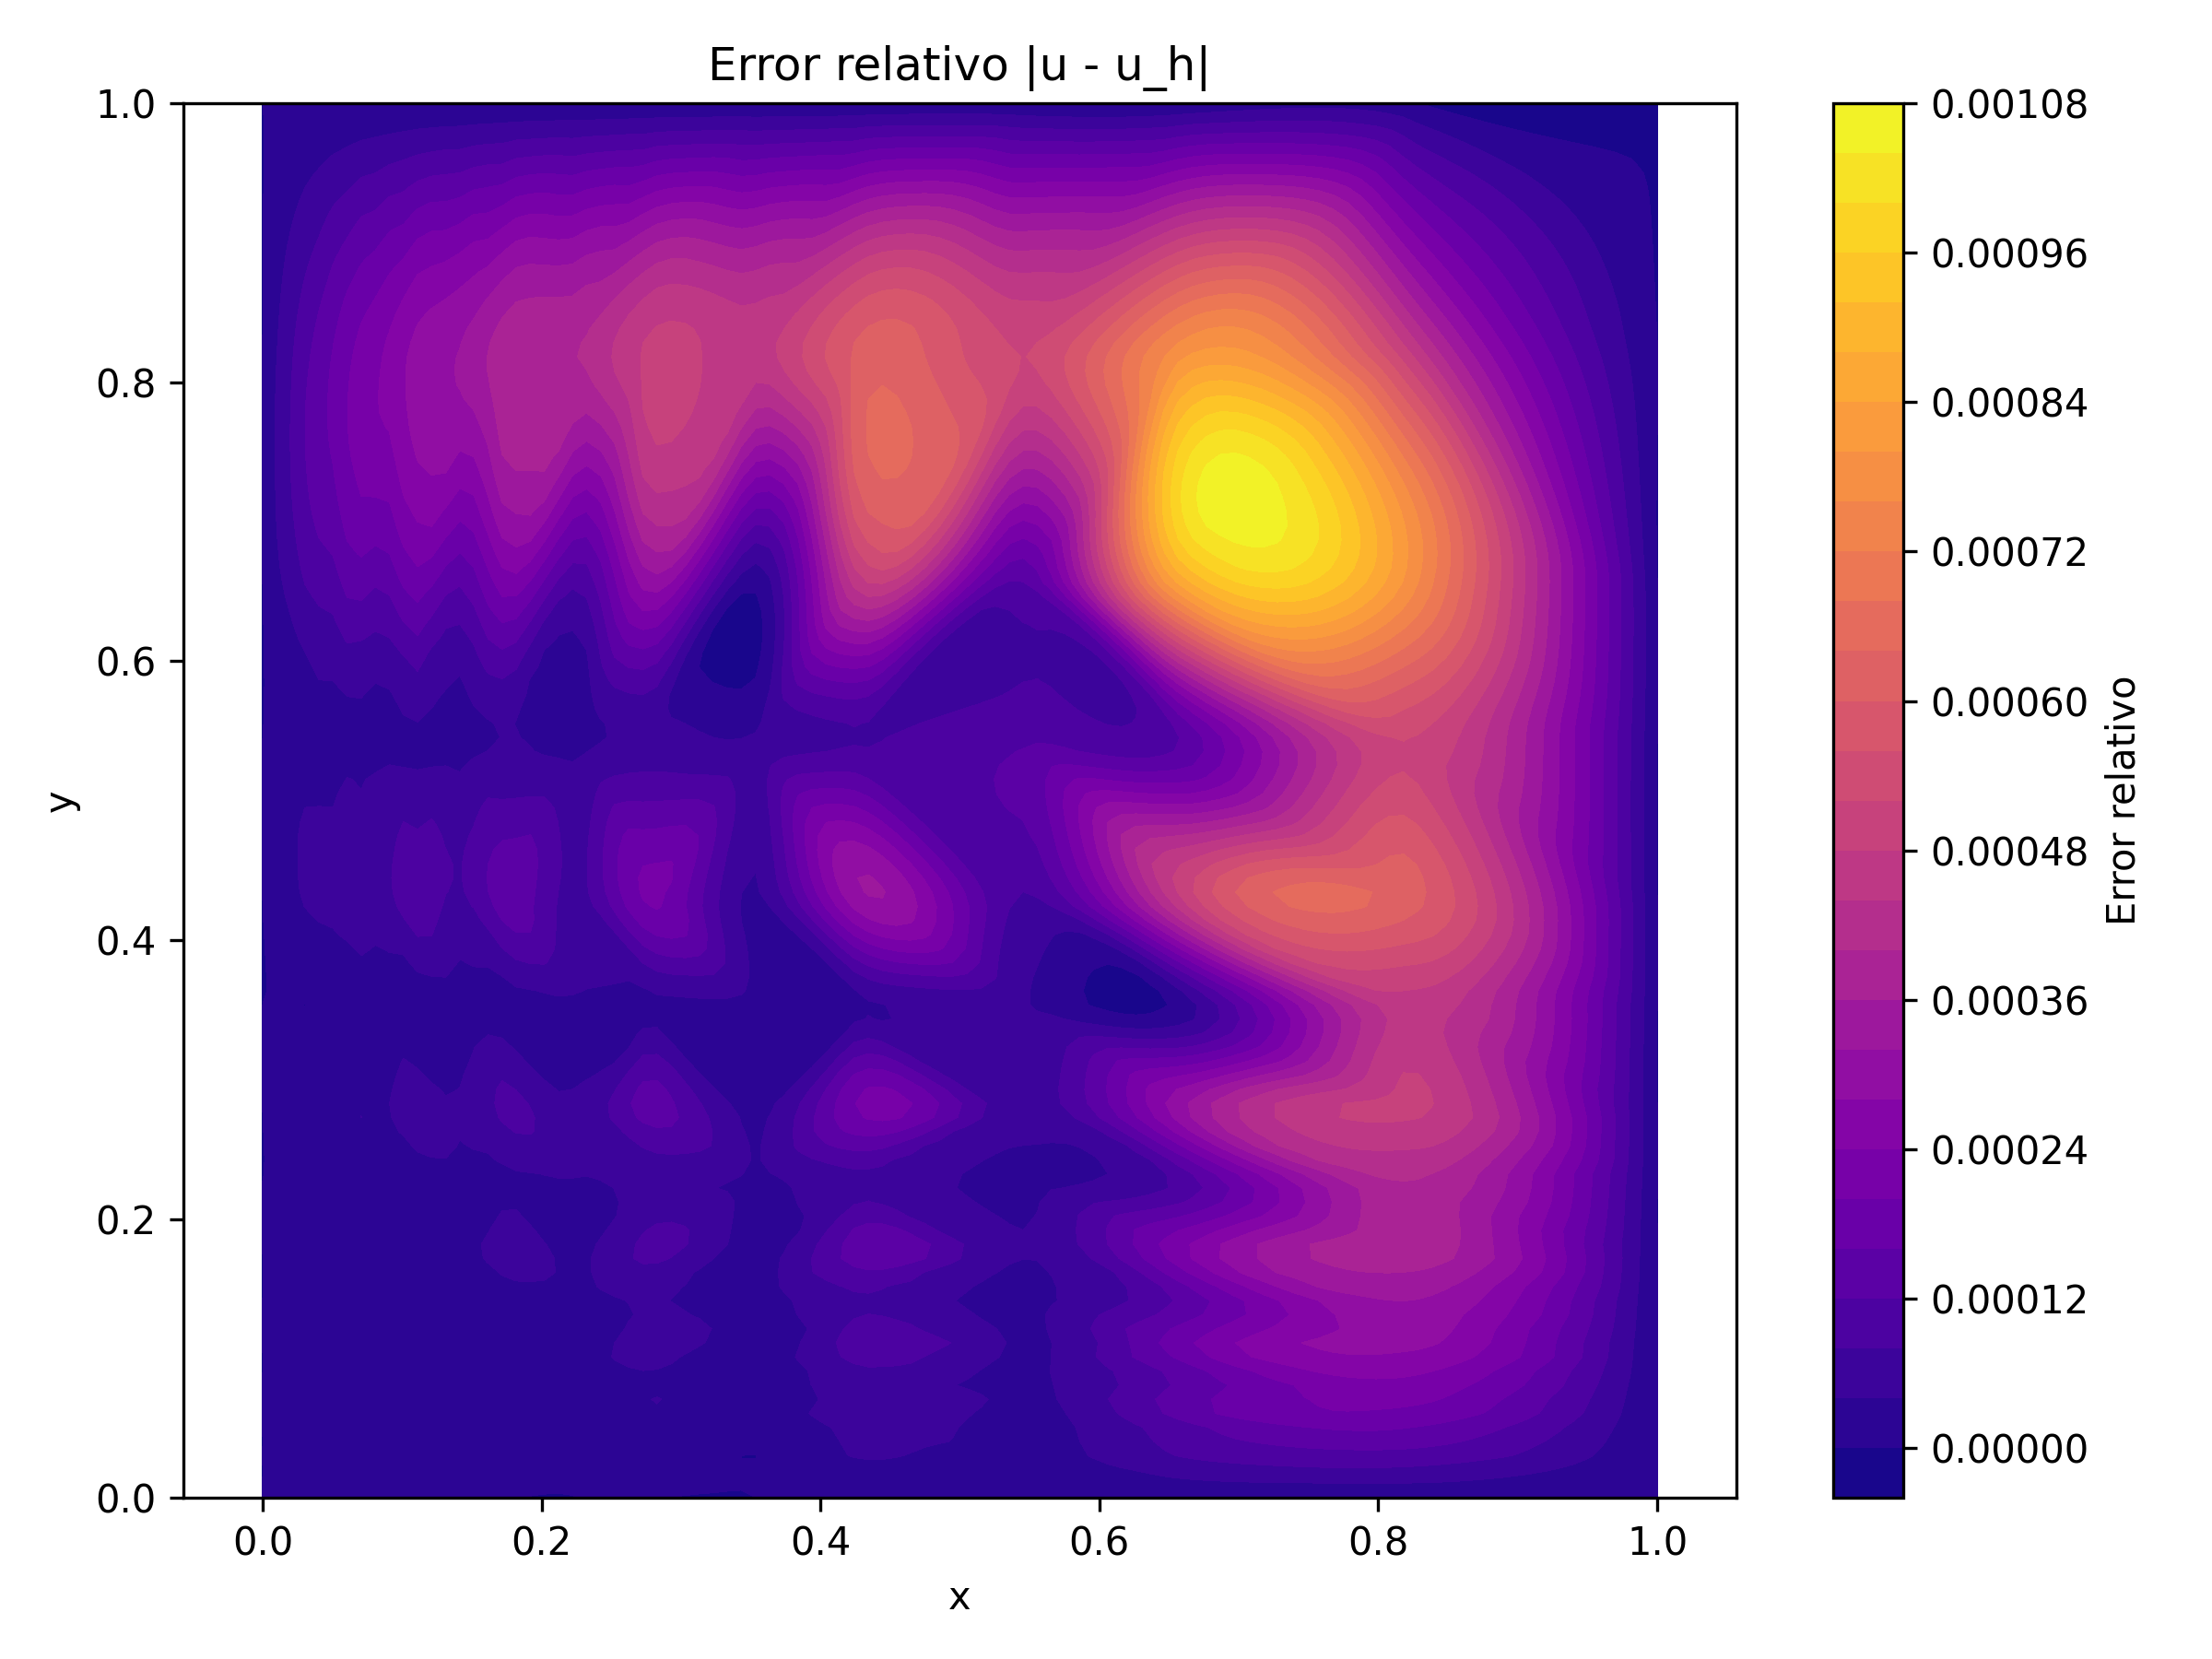
\includegraphics[width=\textwidth]{Graficos/13/LST_relative_error_colormap.png}
        \caption{LST error (N = 10, r = 1.3)}
        \label{fig:lst_error_r1.3}
    \end{subfigure}
    \caption{Relative error for LST elements with $N = 10$ and different values of $r$.}
    \label{fig:lst_error_comparison}
\end{figure}

\begin{figure}[H]
    \centering
    \begin{subfigure}[t]{0.32\textwidth}
        \centering
        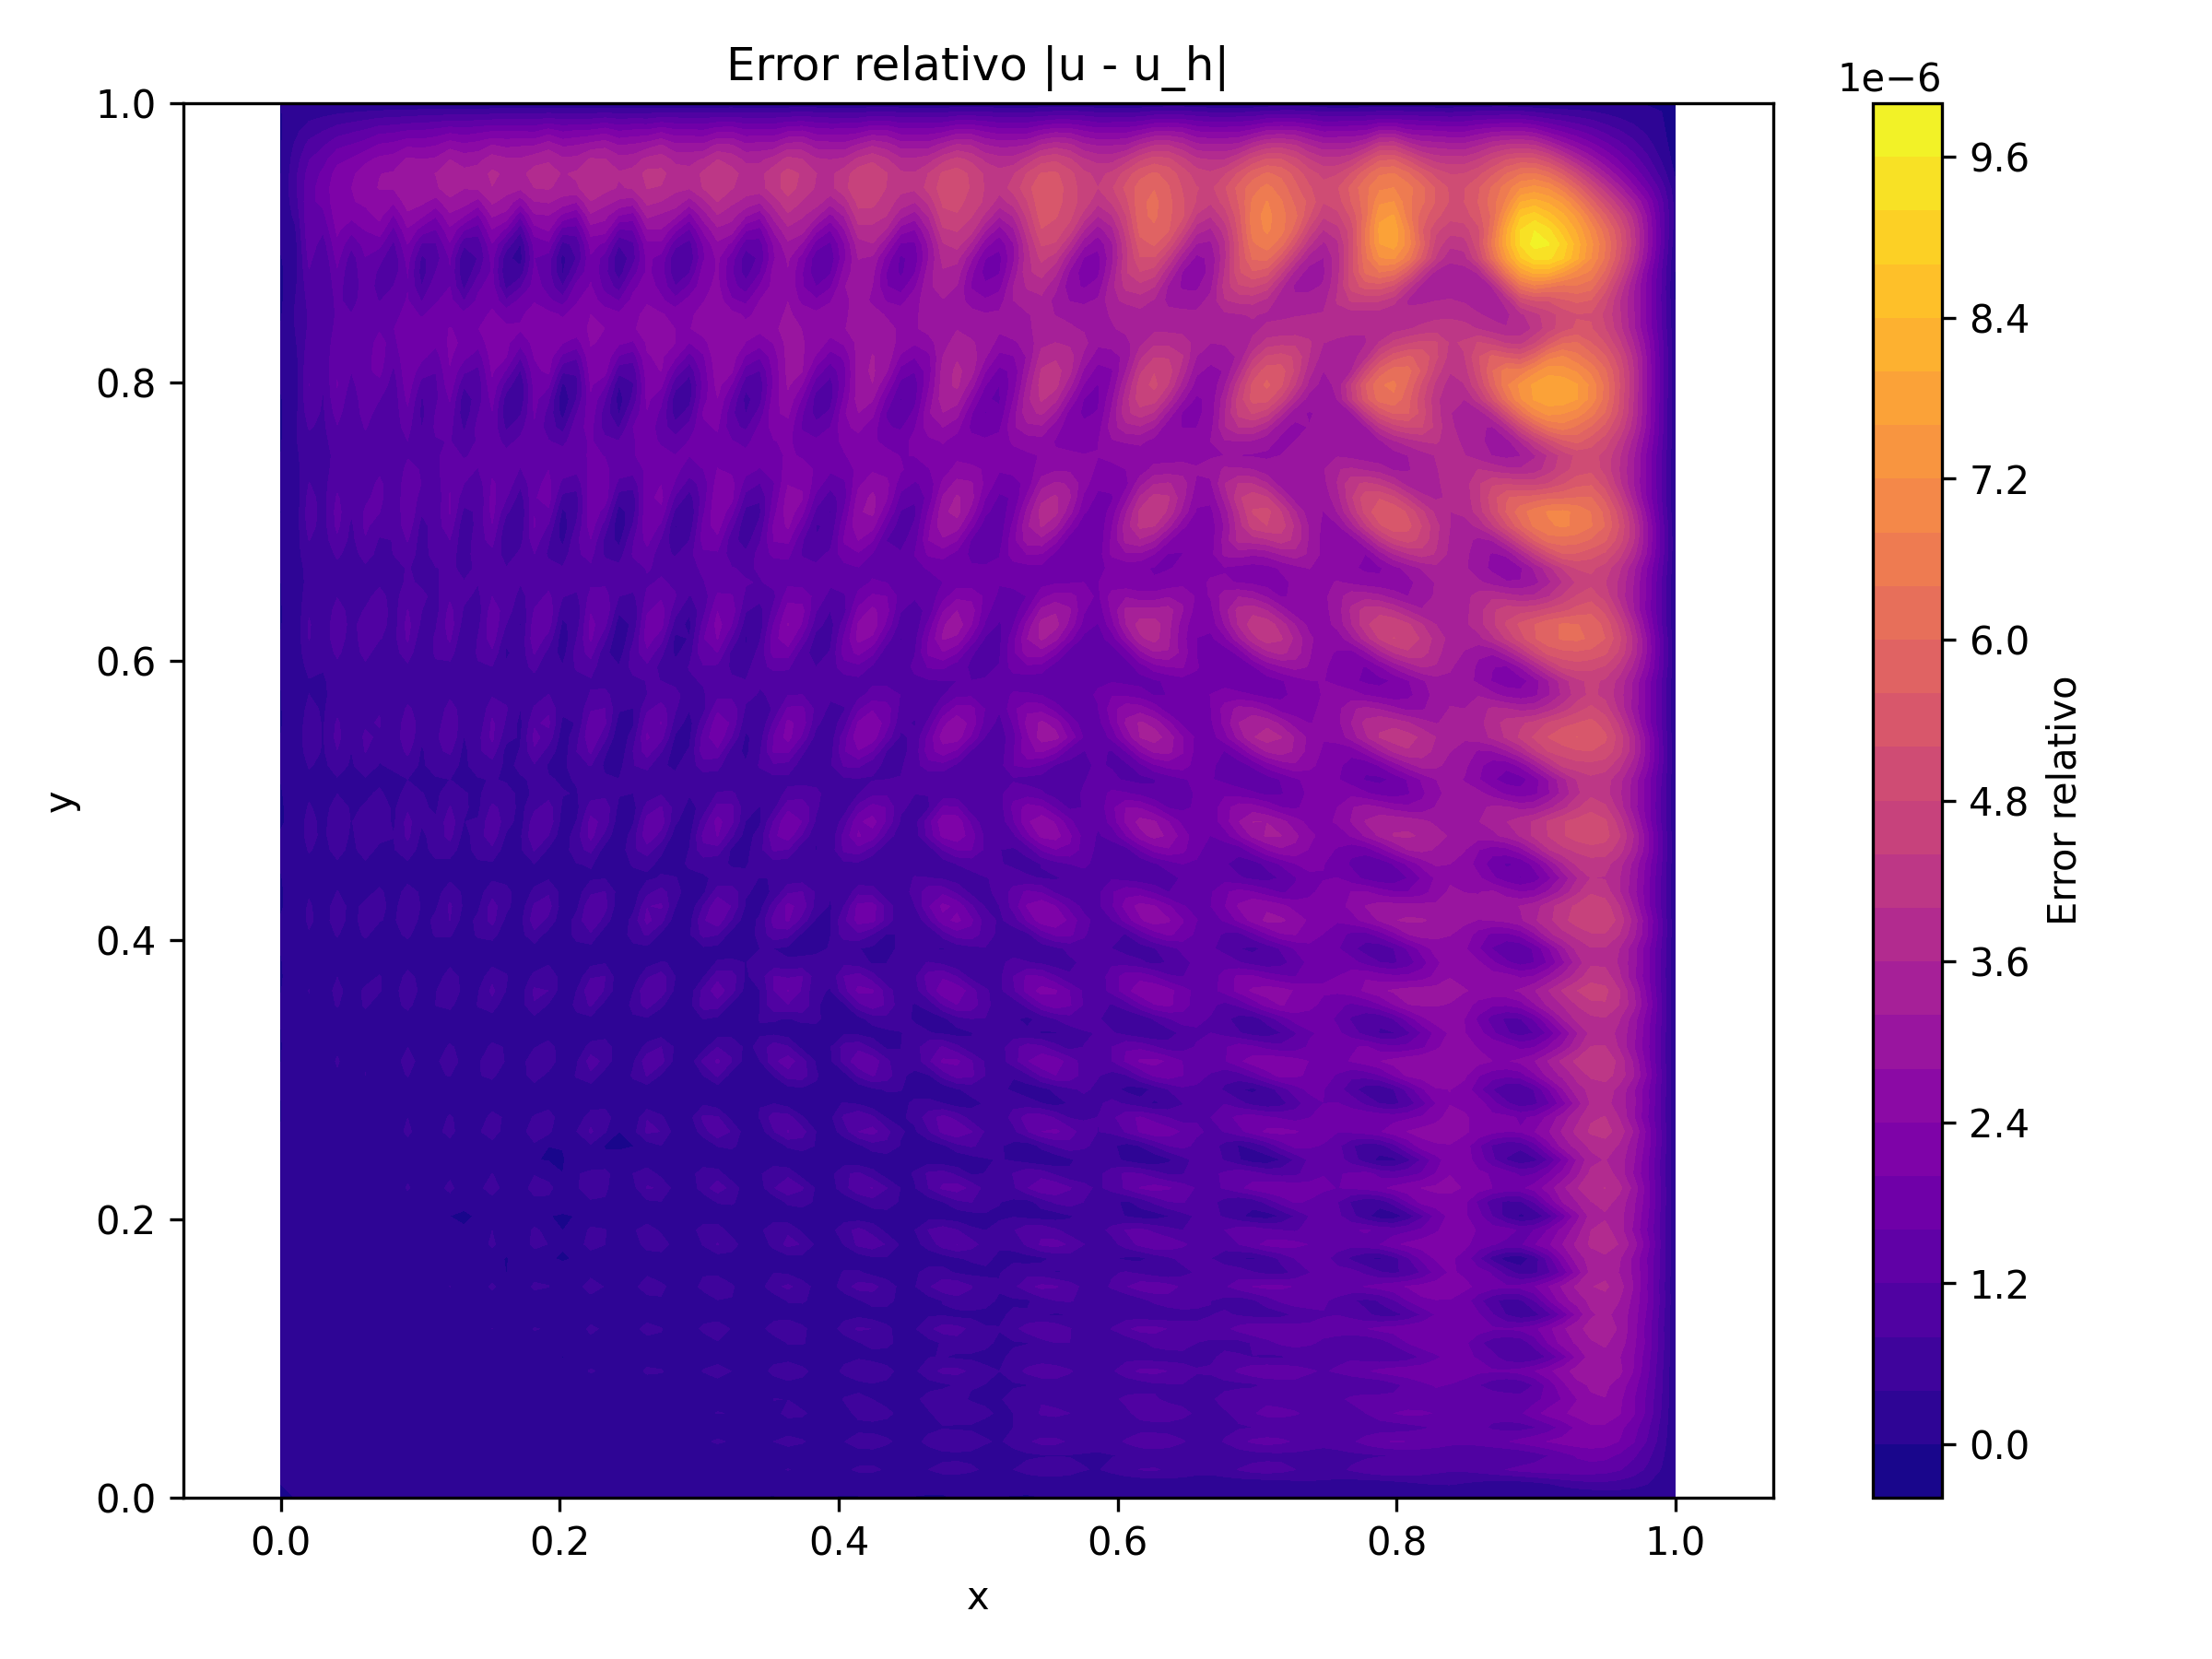
\includegraphics[width=\textwidth]{Graficos/21/LST_relative_error_colormap.png}
        \caption{LST error (N = 20, r = 1.1)}
        \label{fig:lst_error_r1.1_n20}
    \end{subfigure}
    \hfill
    \begin{subfigure}[t]{0.32\textwidth}
        \centering
        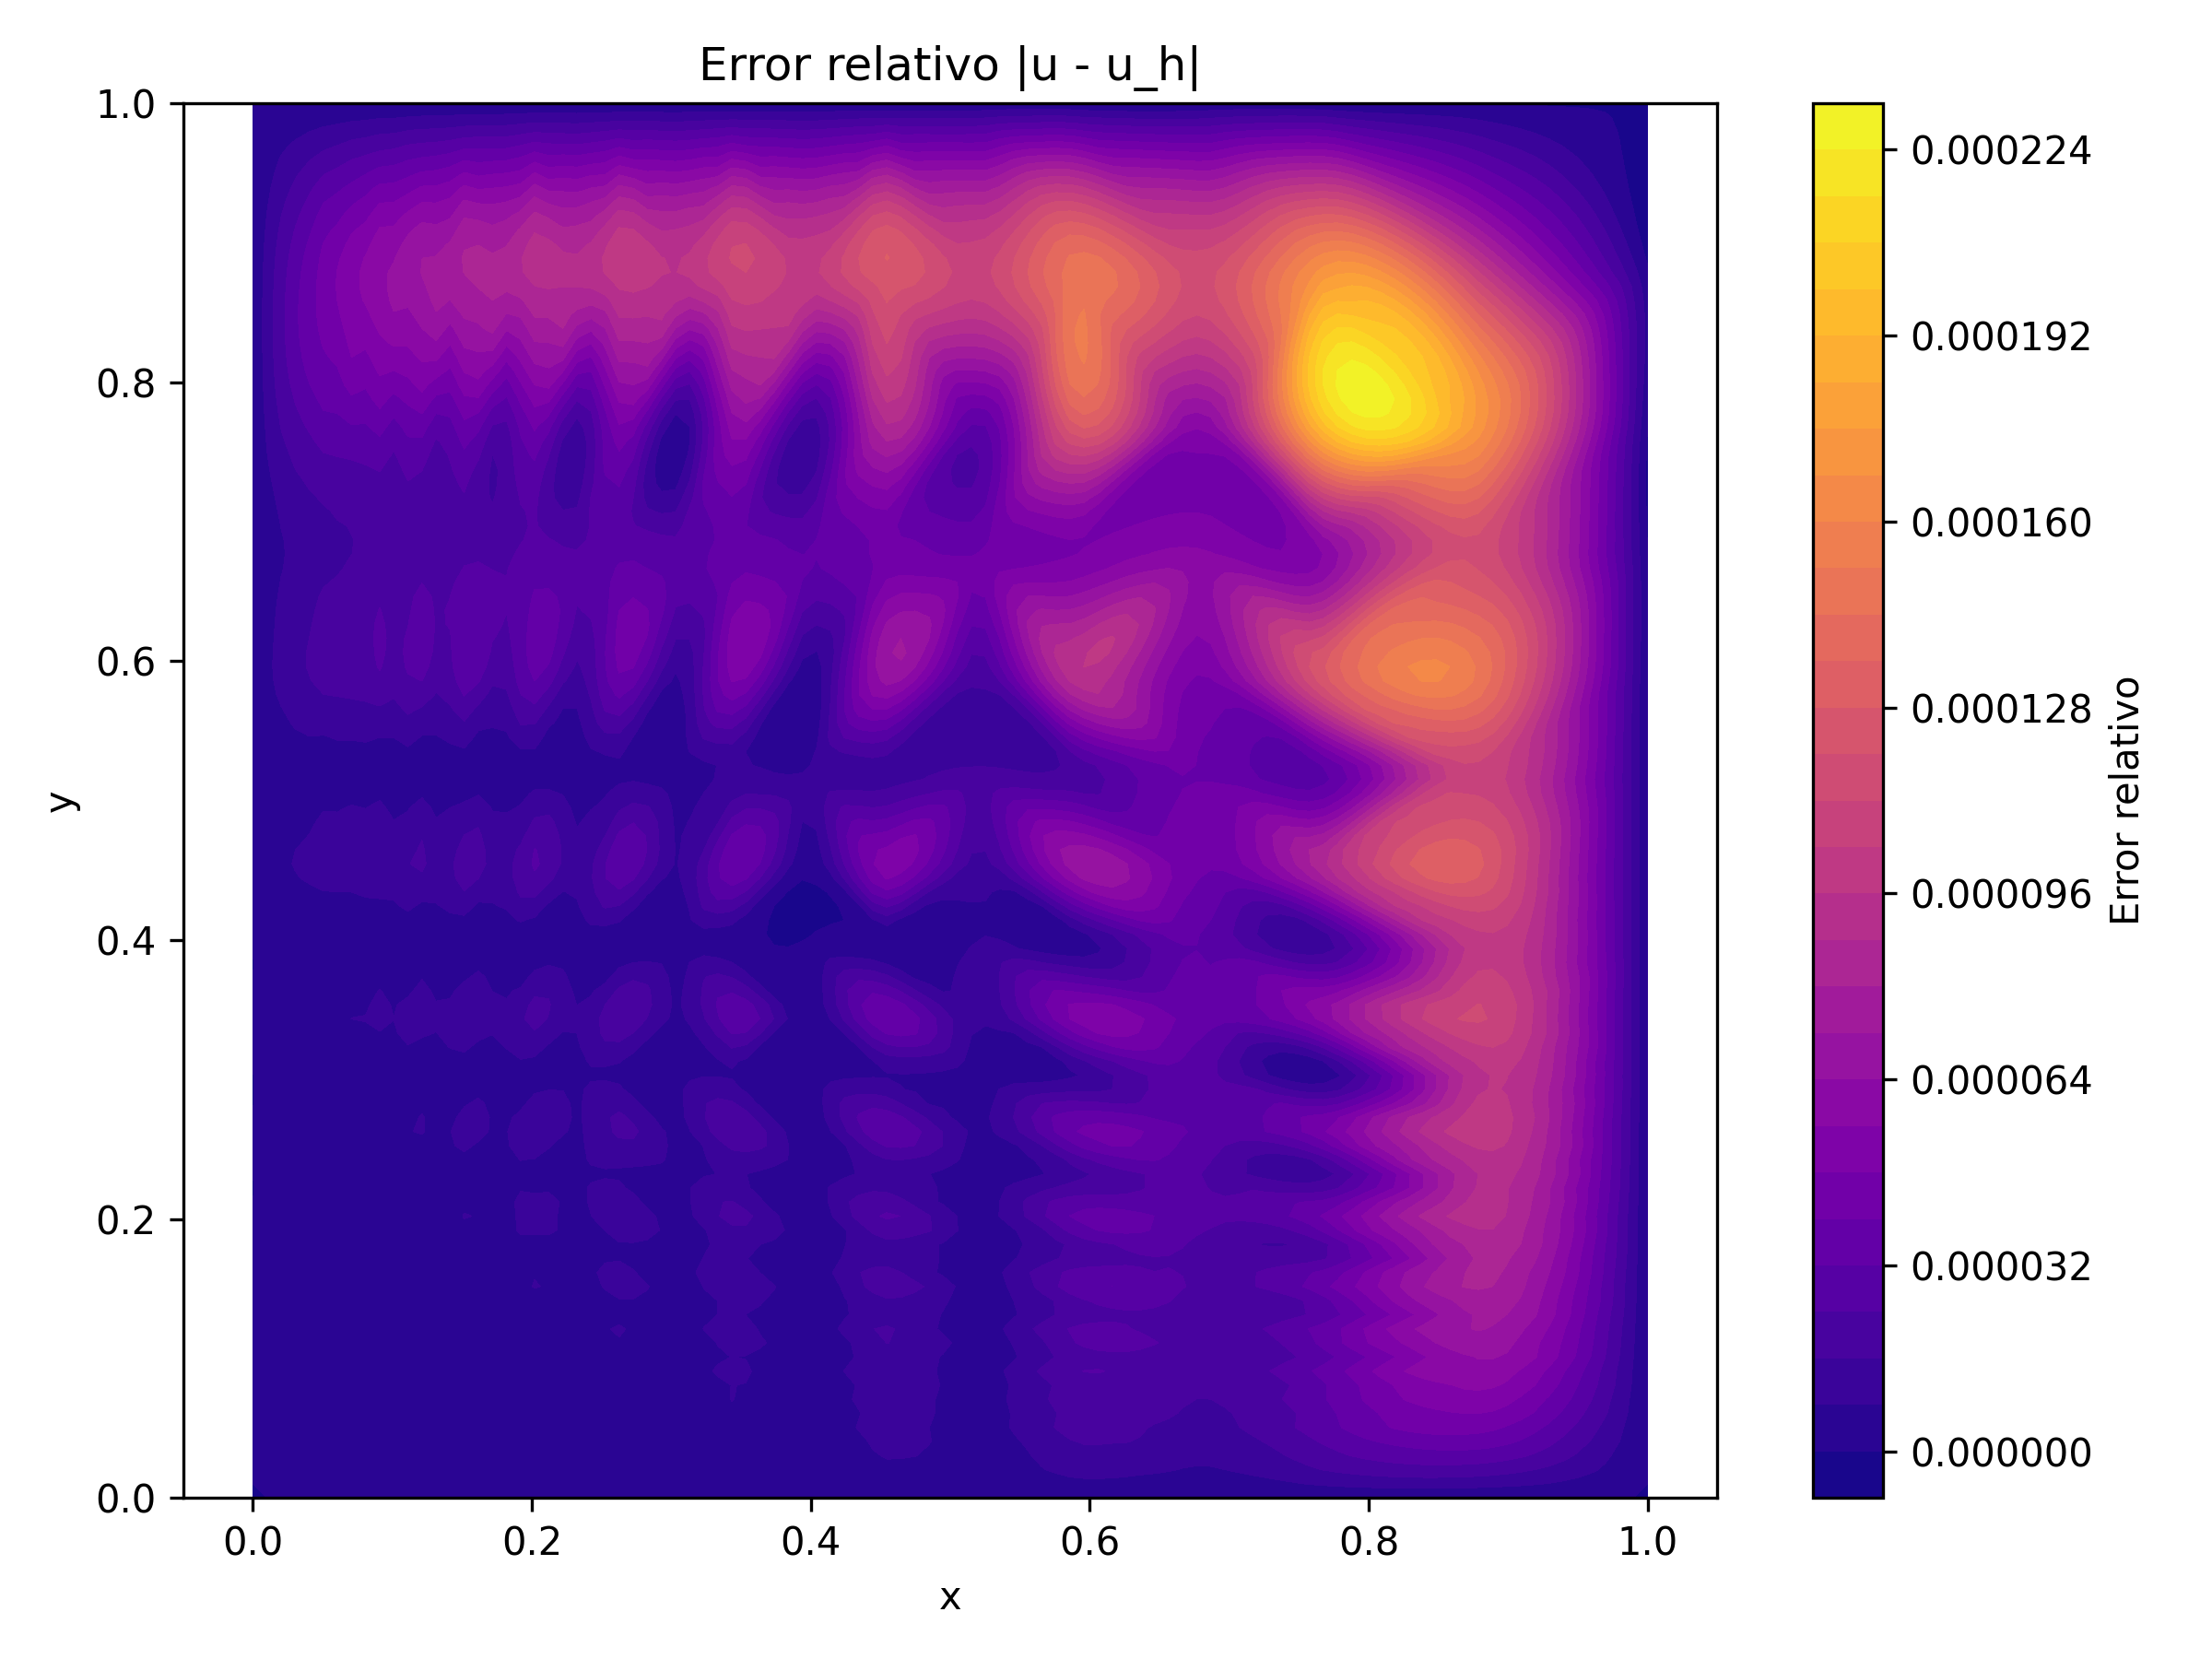
\includegraphics[width=\textwidth]{Graficos/22/LST_relative_error_colormap.png}
        \caption{LST error (N = 20, r = 1.2)}
        \label{fig:lst_error_r1.2_n20}
    \end{subfigure}
    \hfill
    \begin{subfigure}[t]{0.32\textwidth}
        \centering
        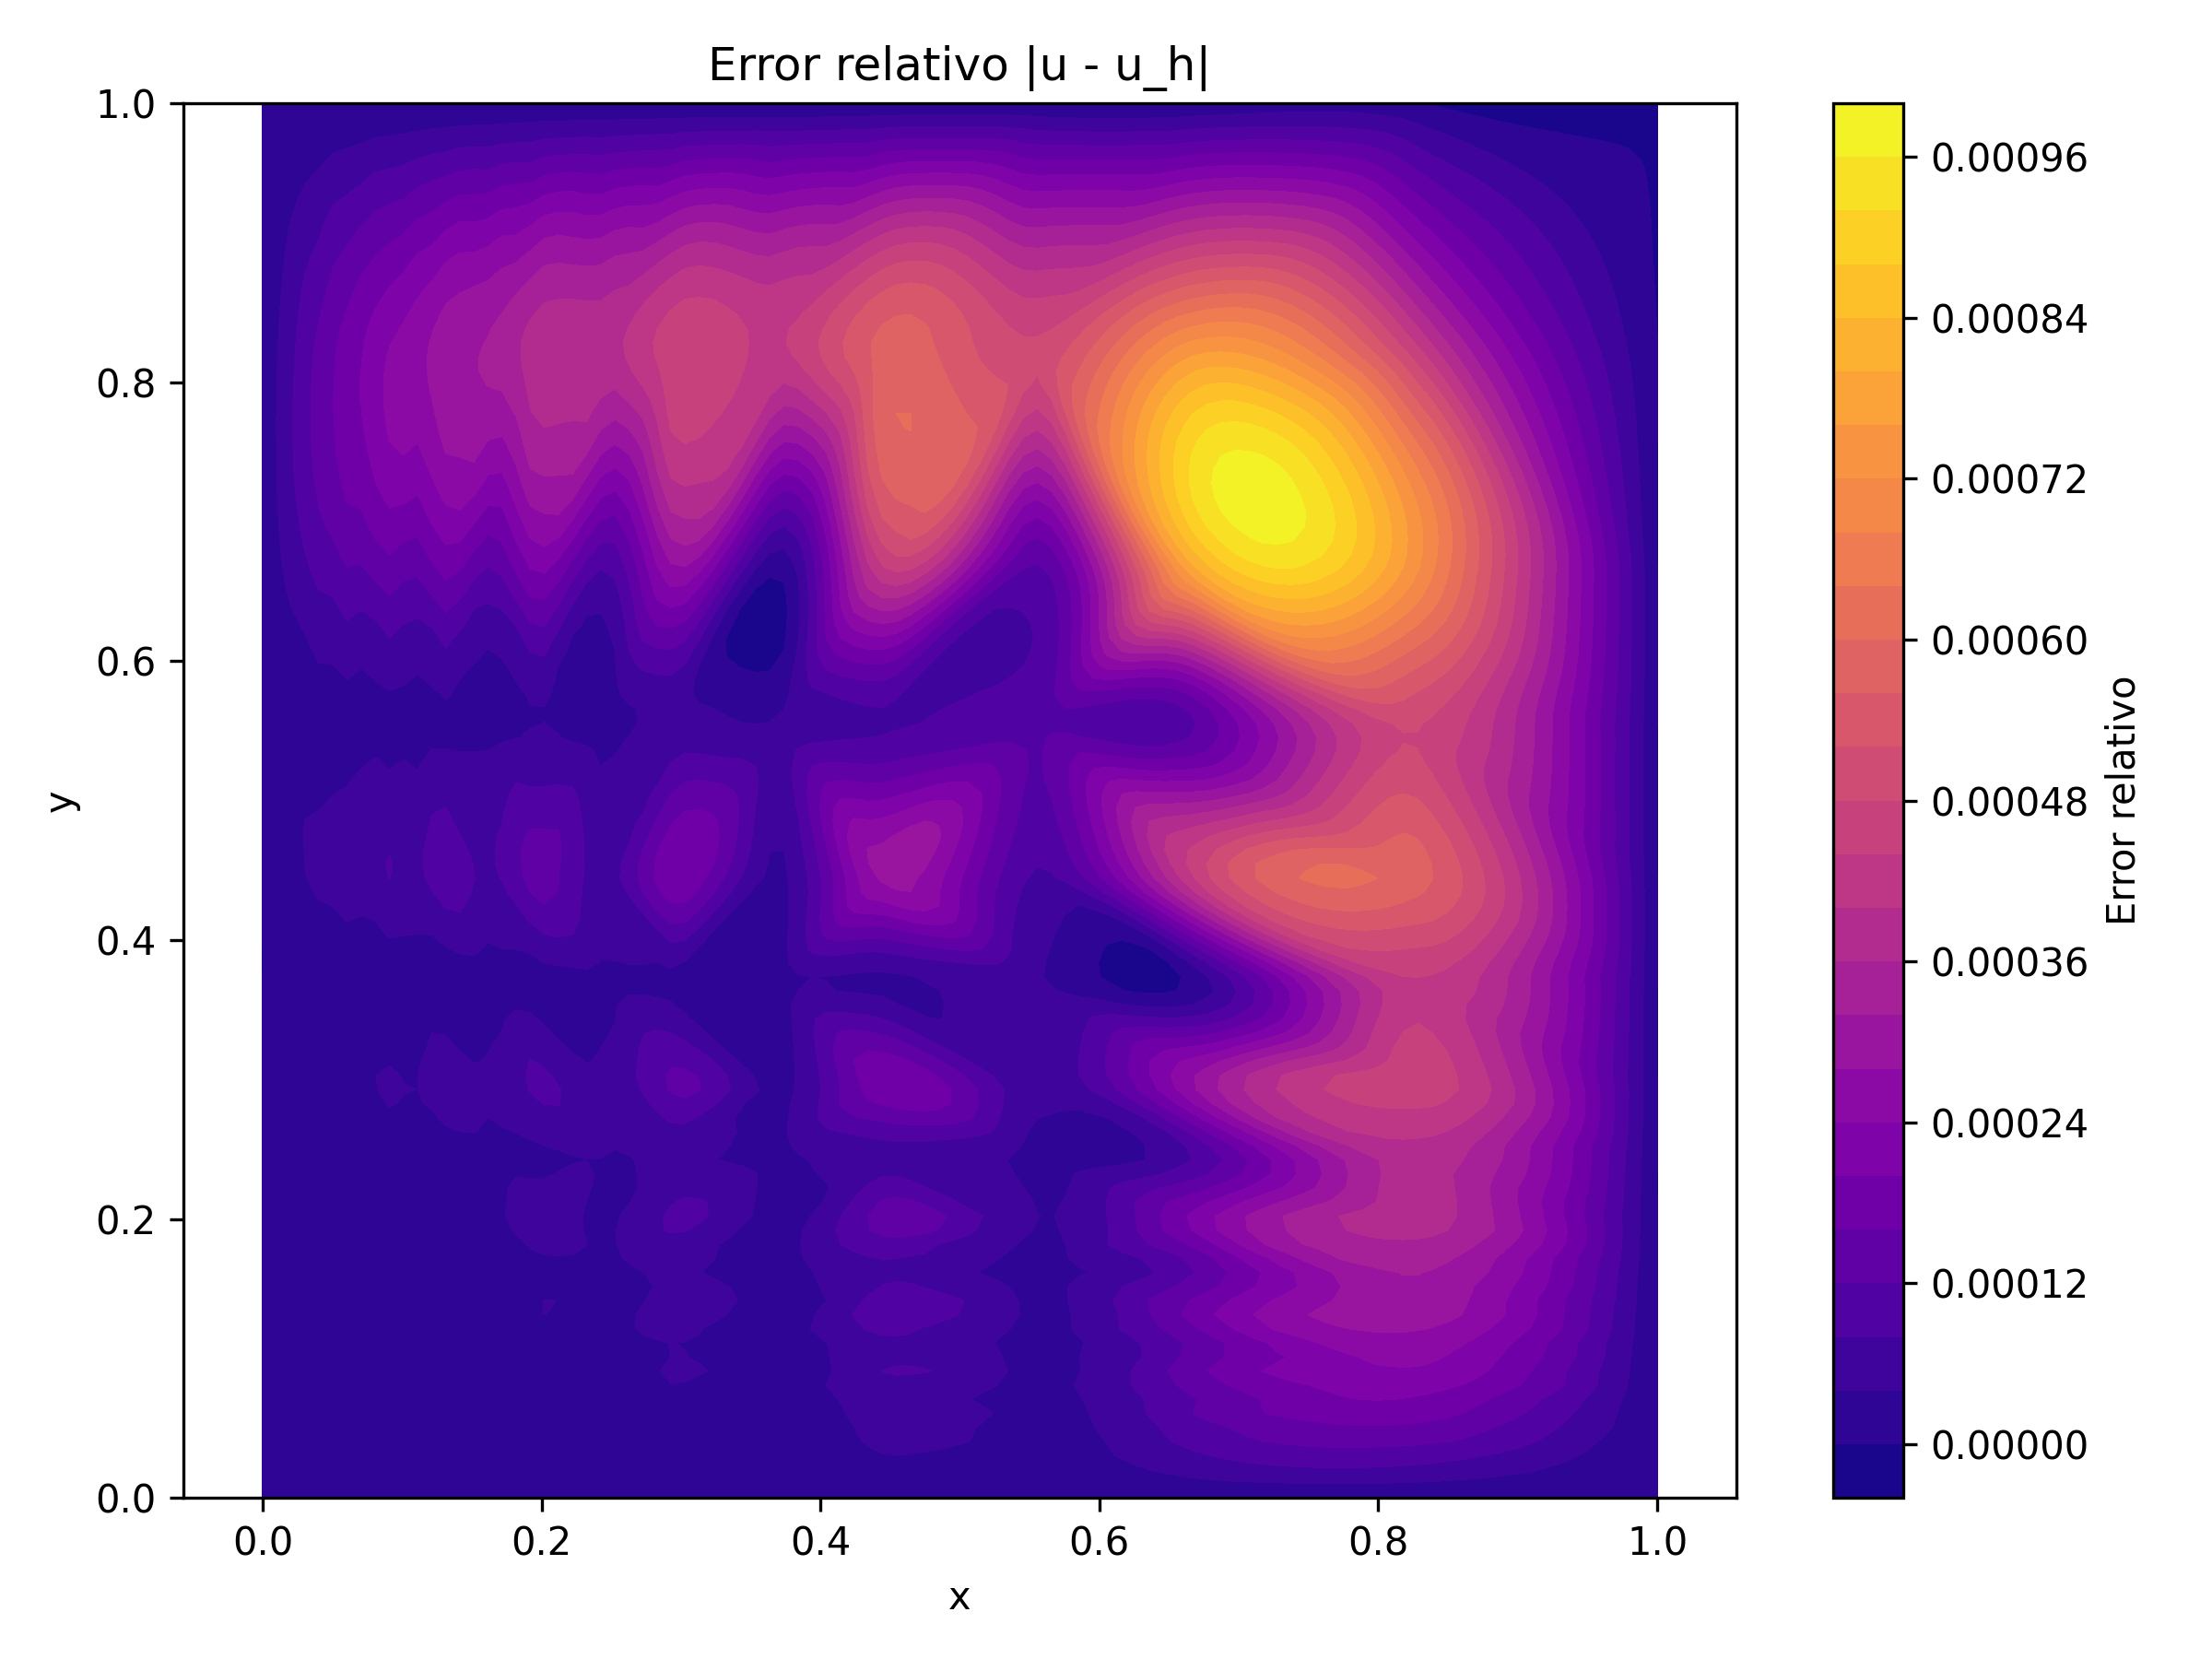
\includegraphics[width=\textwidth]{Graficos/23/LST_relative_error_colormap.png}
        \caption{LST error (N = 20, r = 1.3)}
        \label{fig:lst_error_r1.3_n20}
    \end{subfigure}
    \caption{Relative error for LST elements with $N = 20$ and different values of $r$.}
    \label{fig:lst_error_comparison_n20}
\end{figure}

\begin{figure}[H]
    \centering
    \begin{subfigure}[t]{0.32\textwidth}
        \centering
        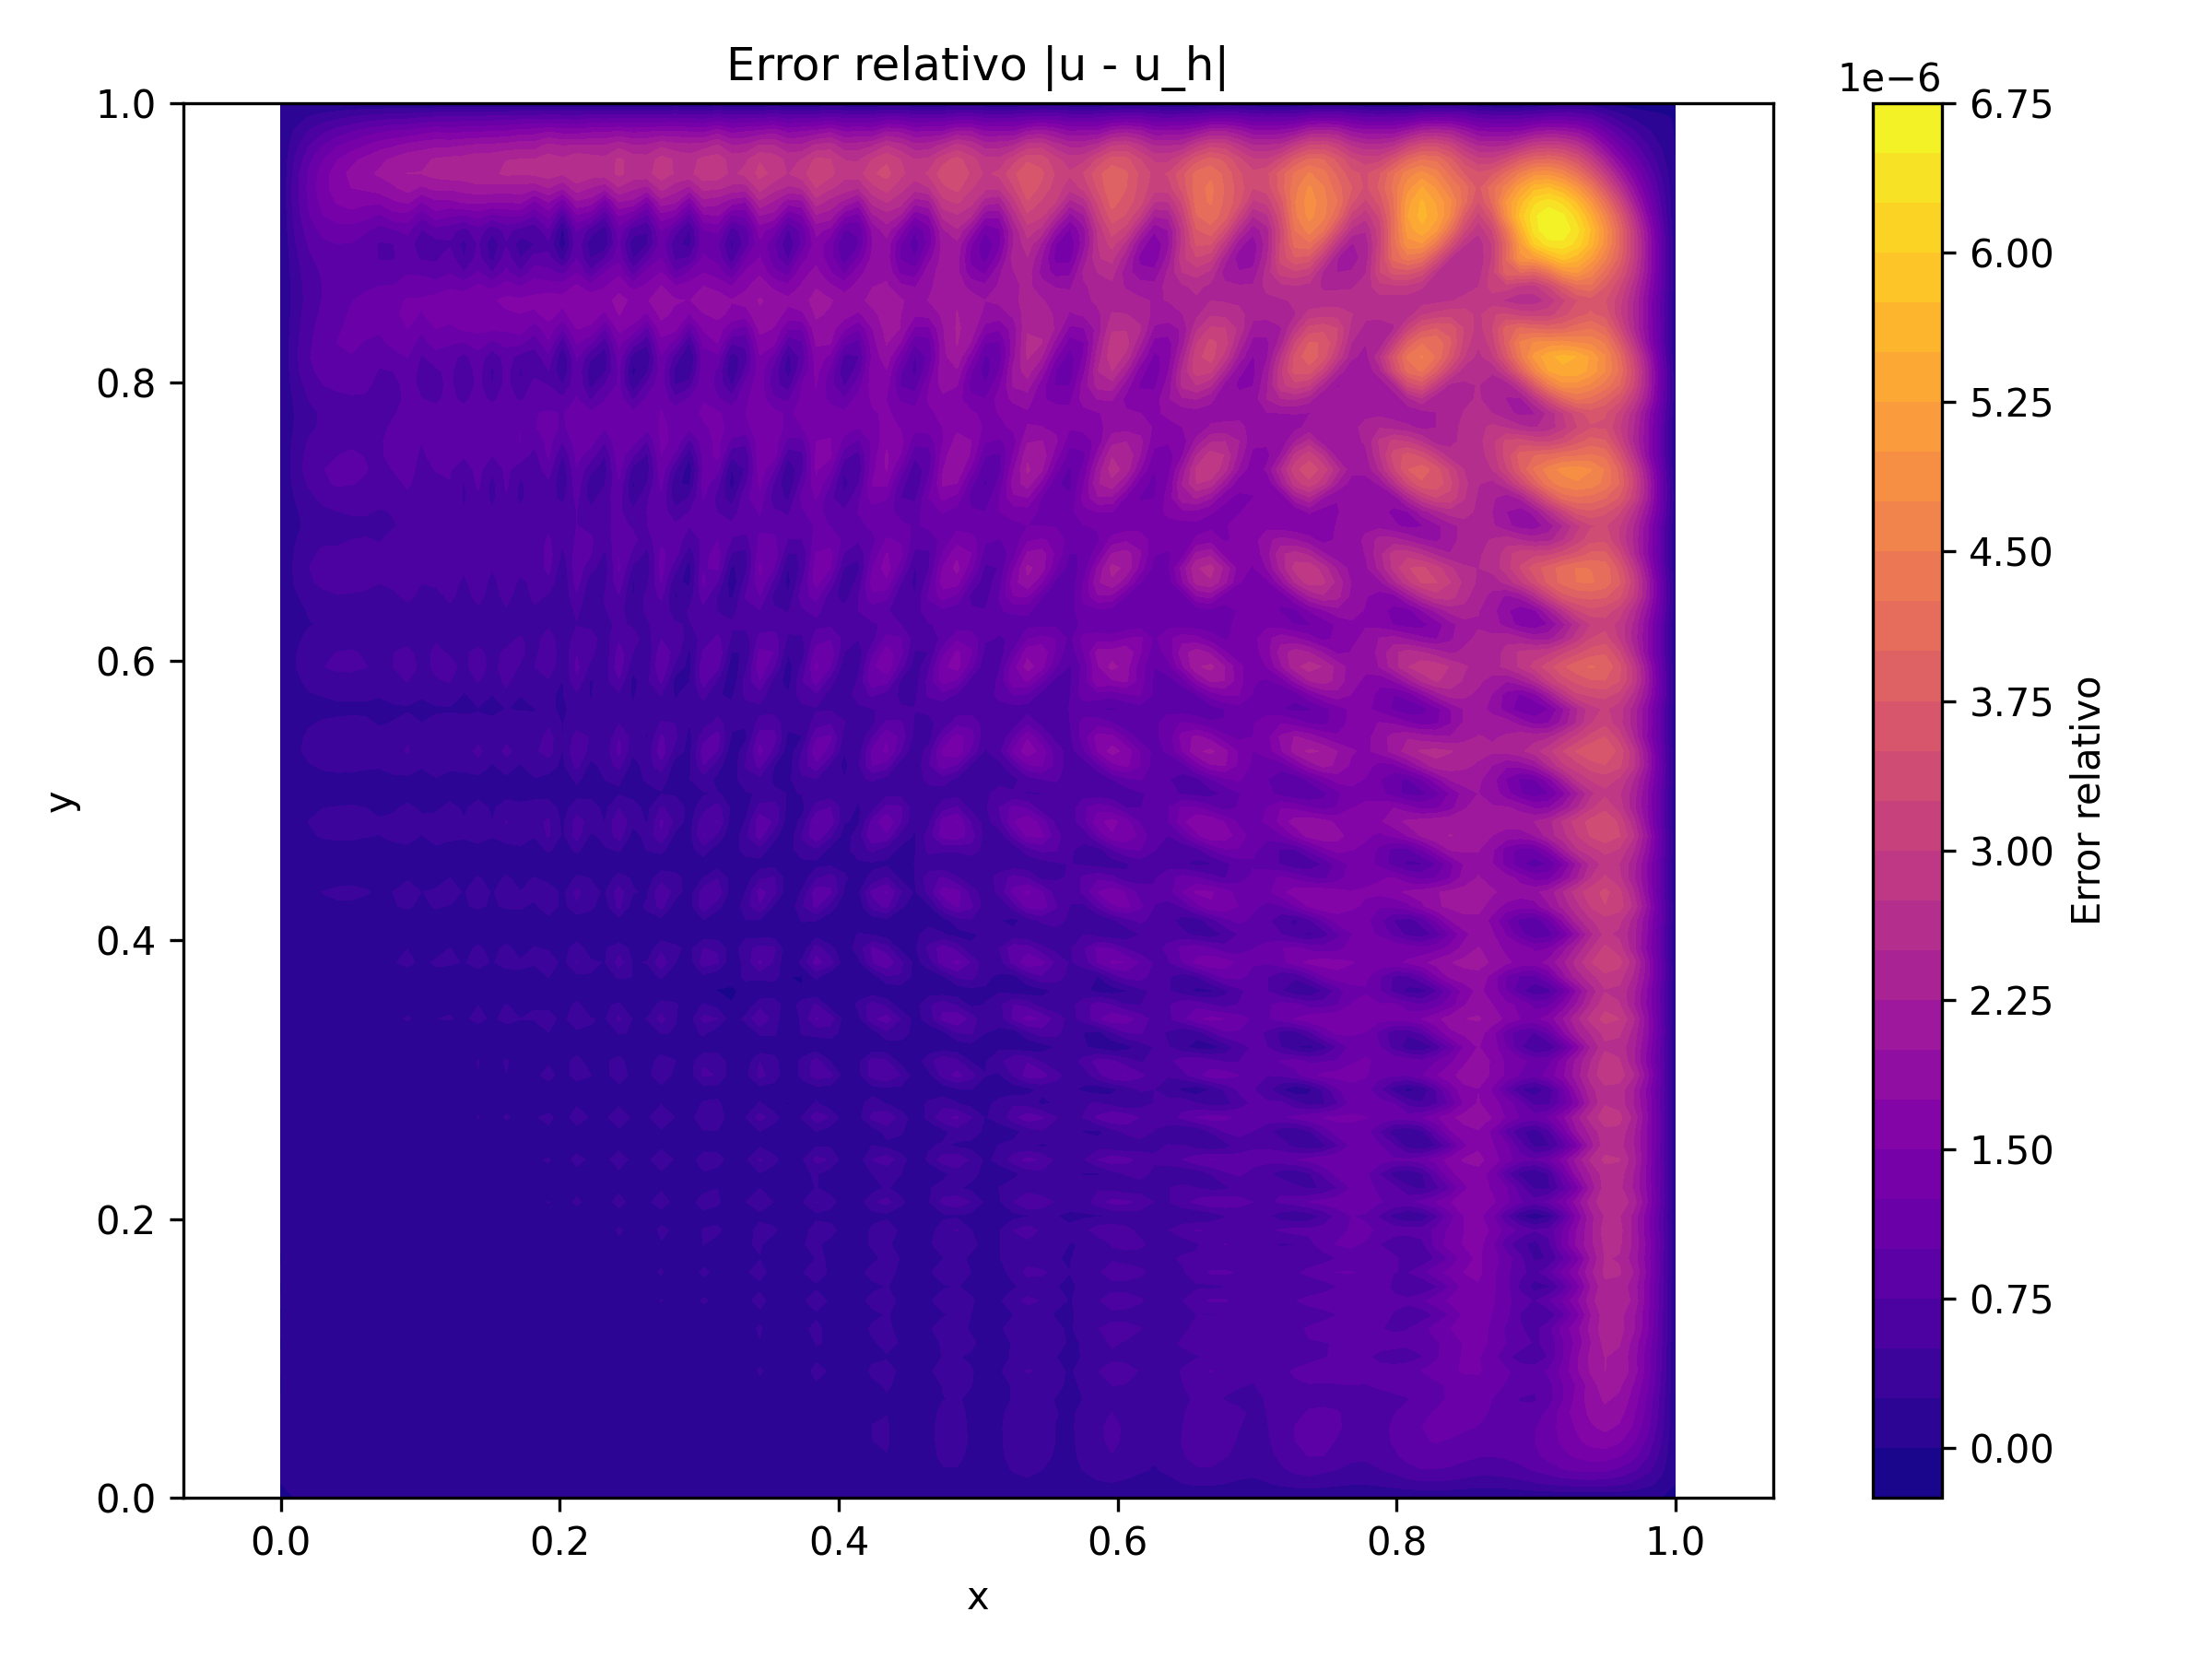
\includegraphics[width=\textwidth]{Graficos/31/LST_relative_error_colormap.png}
        \caption{LST error (N = 30, r = 1.1)}
        \label{fig:lst_error_r1.1_n30}
    \end{subfigure}
    \hfill
    \begin{subfigure}[t]{0.32\textwidth}
        \centering
        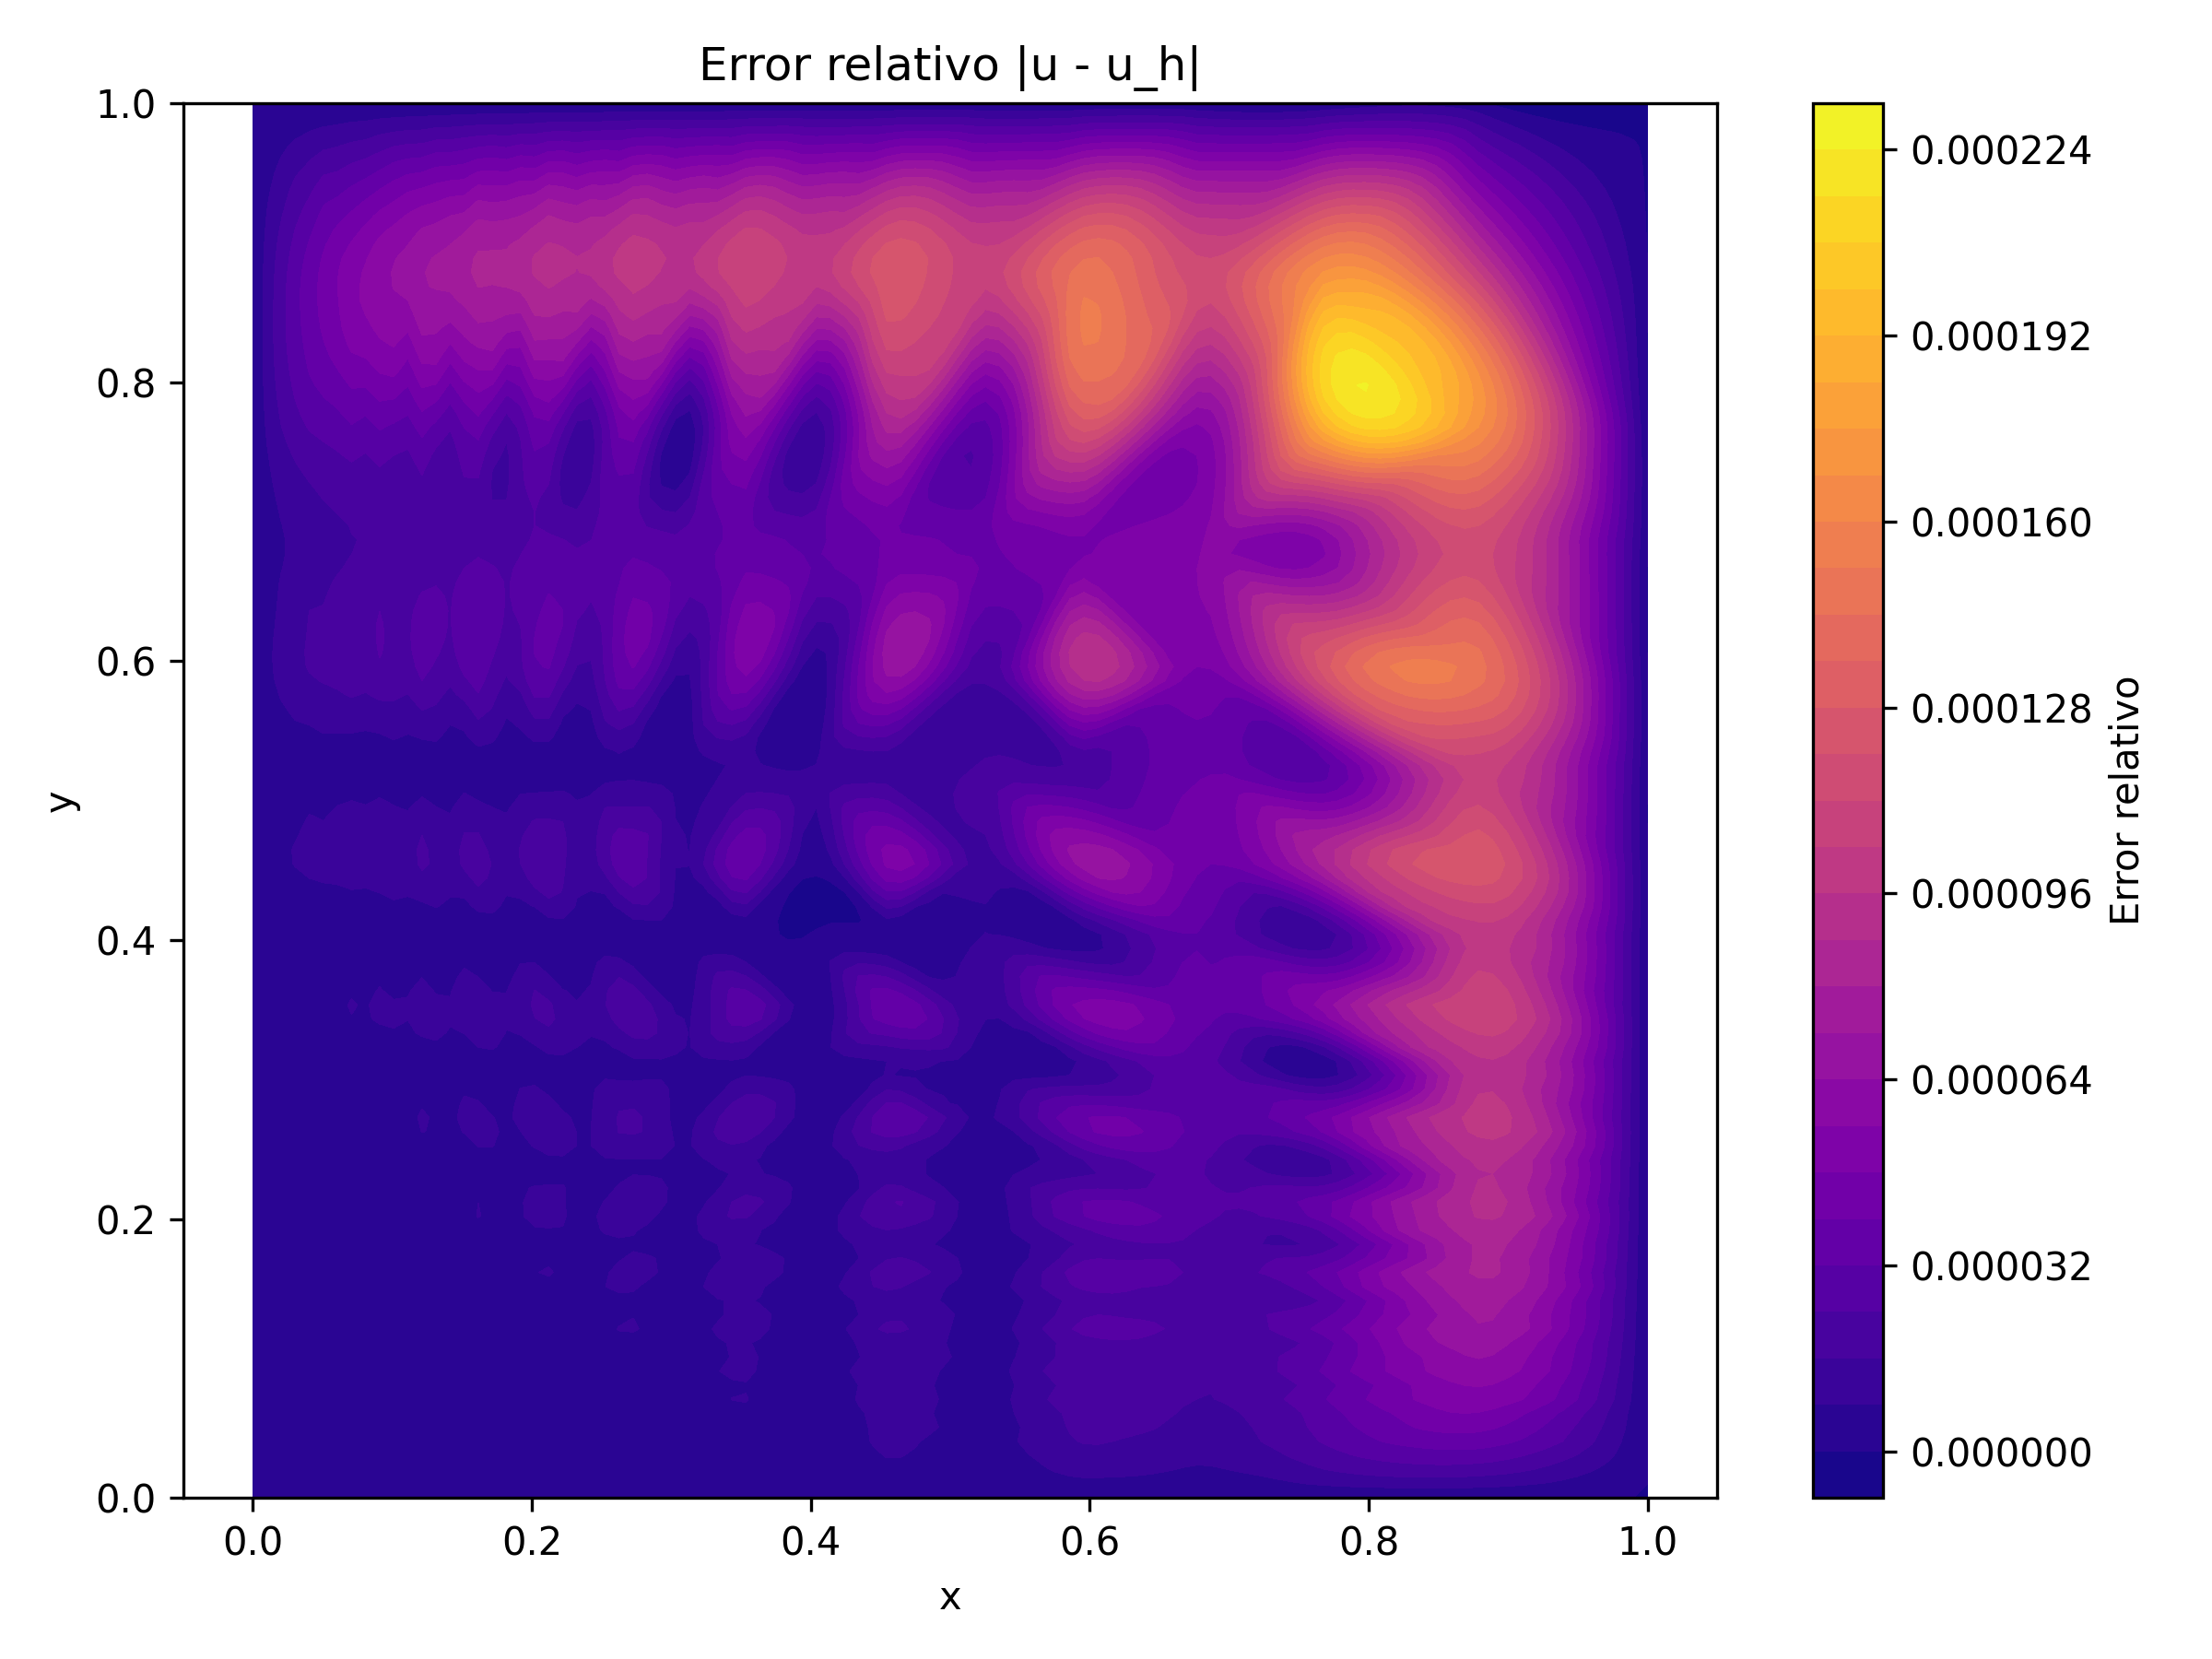
\includegraphics[width=\textwidth]{Graficos/32/LST_relative_error_colormap.png}
        \caption{LST error (N = 30, r = 1.2)}
        \label{fig:lst_error_r1.2_n30}
    \end{subfigure}
    \hfill
    \begin{subfigure}[t]{0.32\textwidth}
        \centering
        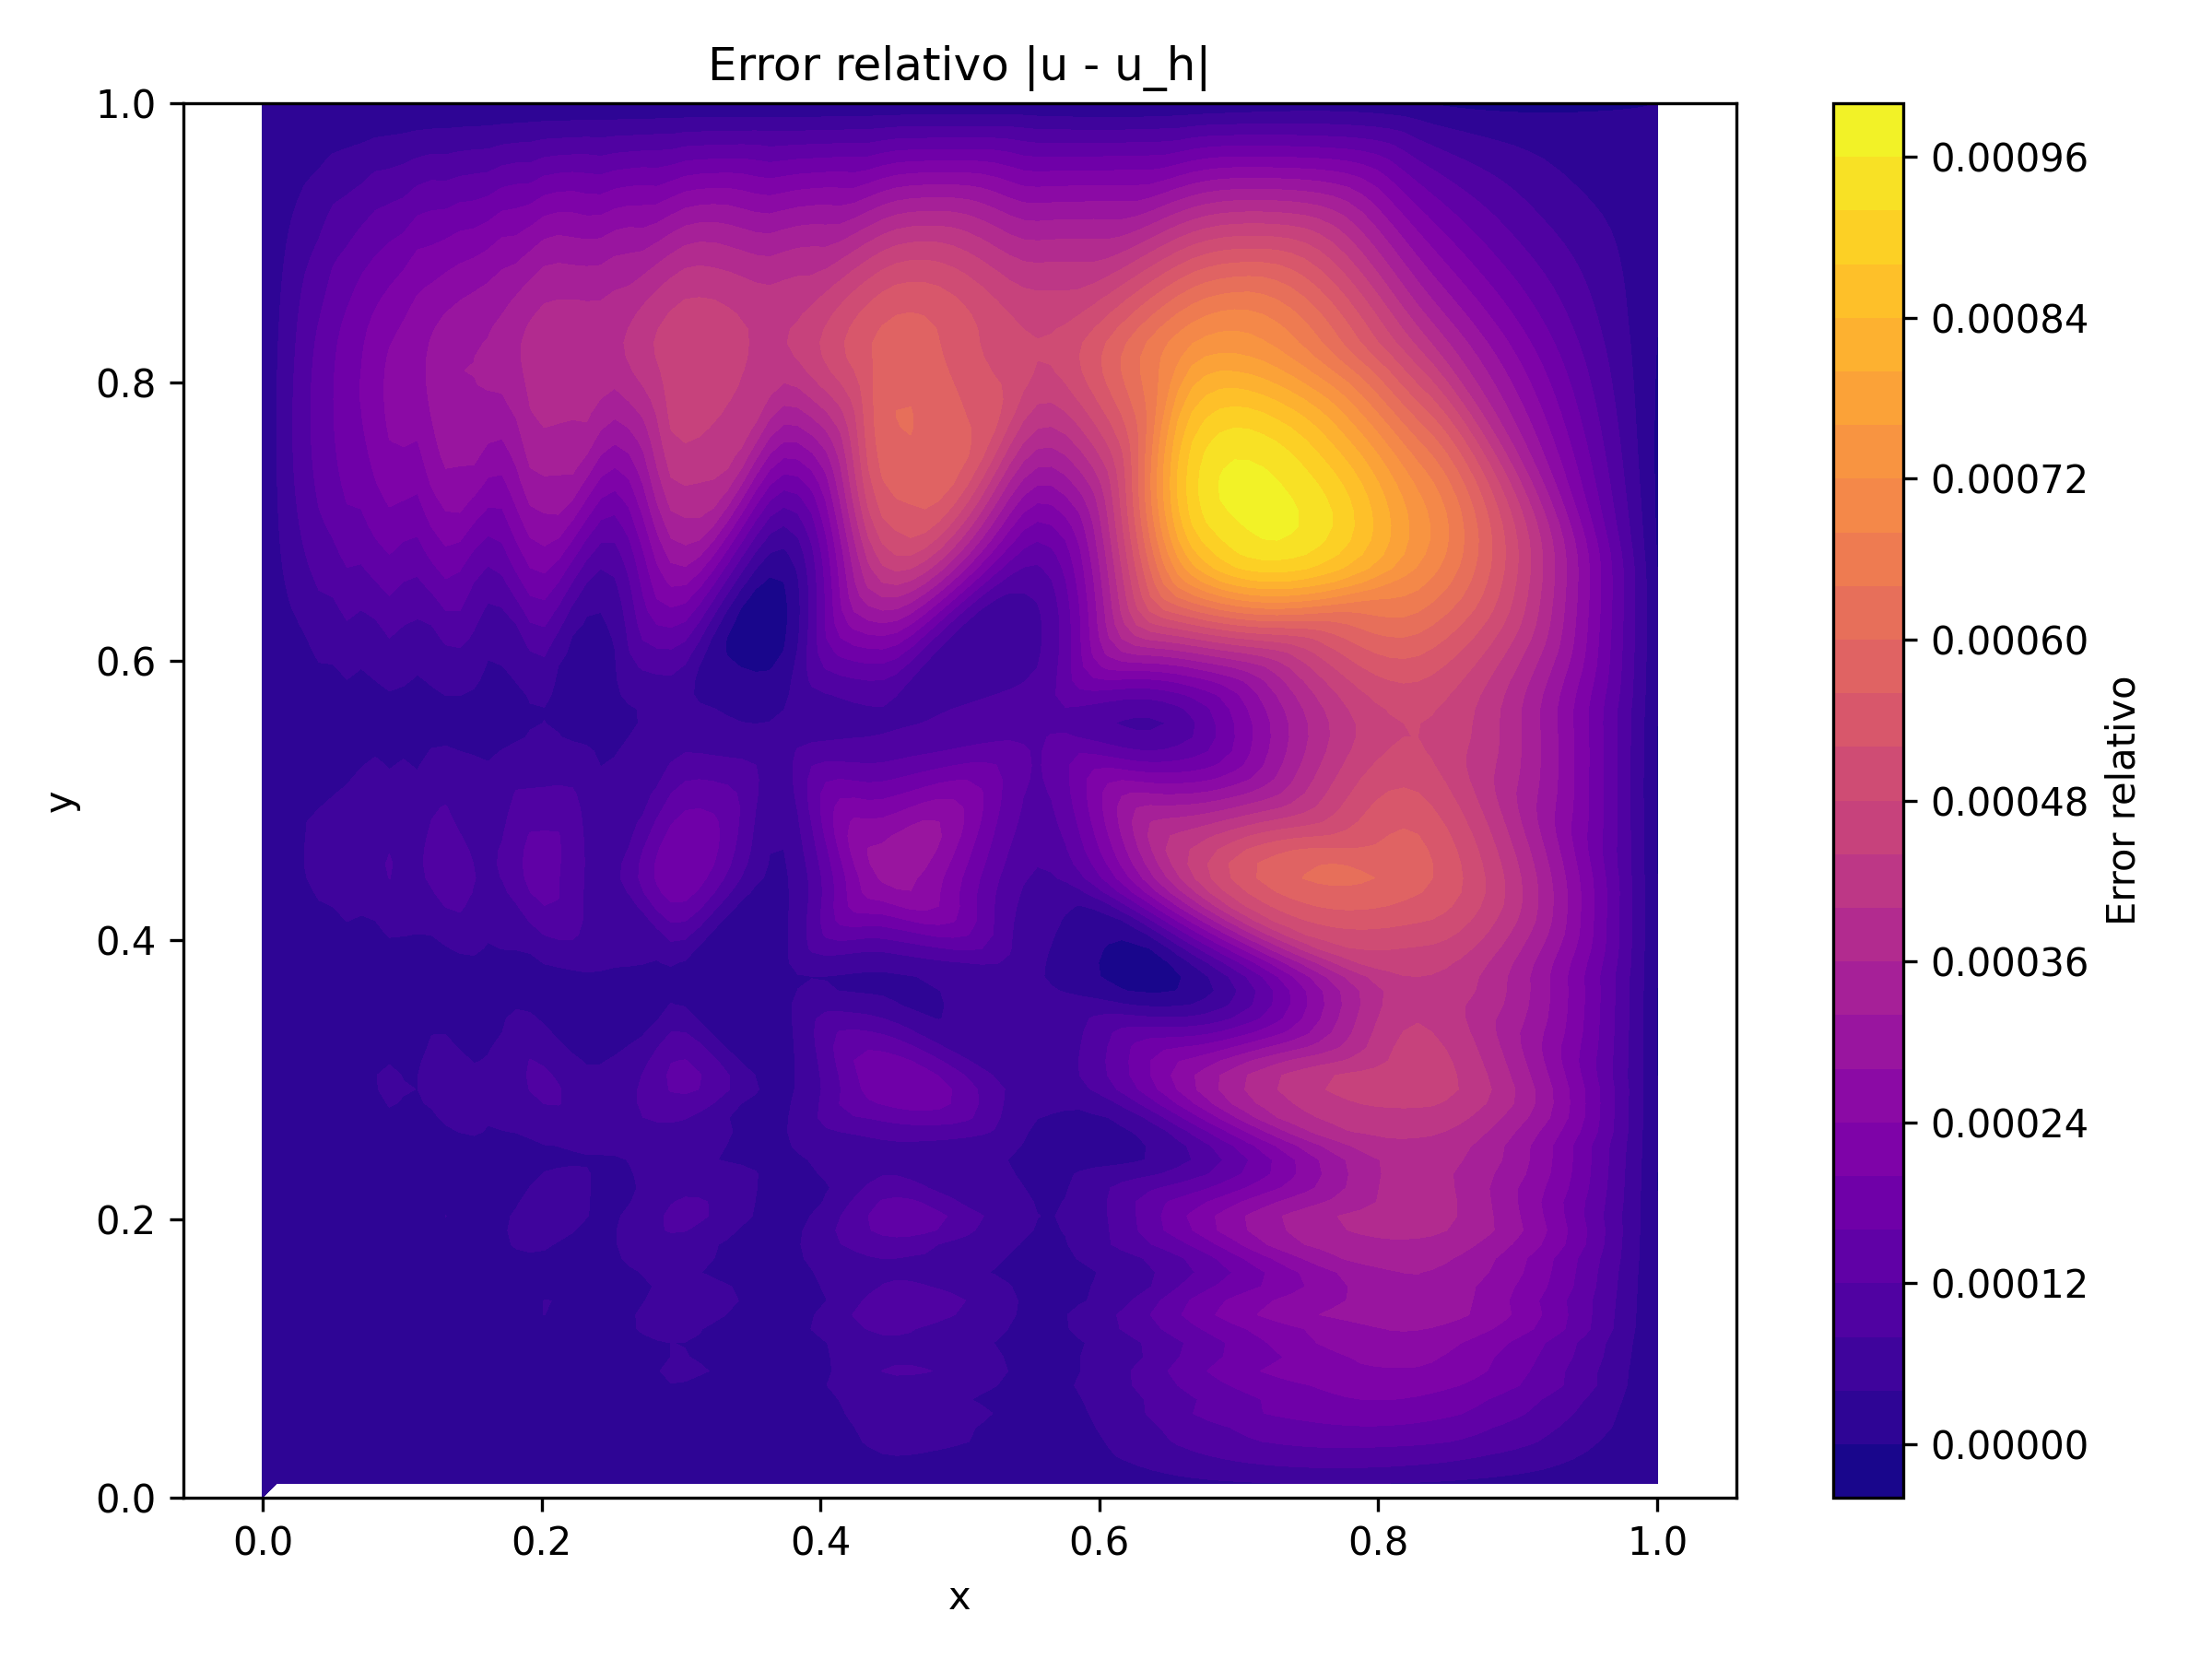
\includegraphics[width=\textwidth]{Graficos/33/LST_relative_error_colormap.png}
        \caption{LST error (N = 30, r = 1.3)}
        \label{fig:lst_error_r1.3_n30}
    \end{subfigure}
    \caption{Relative error for LST elements with $N = 30$ and different values of $r$.}
    \label{fig:lst_error_comparison_n30}
\end{figure}

For LST elements, a similar behavior is observed: the relative errors tend to be higher in the elements with the largest size, which are located in the upper right corner of the mesh. This region is also farther from the boundary conditions, which contributes to the accumulation of error. Despite the quadratic interpolation capabilities of LST elements, the lack of refinement in those zones leads to a reduction in accuracy, especially in capturing gradients of the solution. This pattern can be clearly seen in the figures displaying the relative error for LST elements.

\subsection{Comparative Analysis}

In the following tables, we summarize the relative errors obtained for both CST and LST elements across different values of $N$ (number of elements) and $r$ (refinement factor). The maximum, average, and minimum errors are presented to provide a comprehensive view of the performance of each element type.

\begin{table}[H]
\centering
\caption{Relative errors for CST elements for different values of $N$ and $r$.}
\begin{tabular}{|c|c|c|c|c|}
\hline
\textbf{$N$} & \textbf{$r$} & \textbf{Max Error} & \textbf{Avg Error} & \textbf{Min Error} \\
\hline
\multirow{3}{*}{10}
& 1.1 & 4.94e-01 & 1.66e-01 & 0.00e+00 \\
& 1.2 & 4.83e-01 & 1.14e-01 & 0.00e+00 \\
& 1.3 & 4.30e-01 & 7.23e-02 & 0.00e+00 \\
\hline
\multirow{3}{*}{20}
& 1.1 & 4.98e-01 & 1.57e-01 & 0.00e+00 \\
& 1.2 & 4.83e-01 & 5.67e-02 & 0.00e+00 \\
& 1.3 & 4.33e-01 & 2.45e-02 & 0.00e+00 \\
\hline
\multirow{3}{*}{30}
& 1.1 & 4.96e-01 & 1.26e-01 & 0.00e+00 \\
& 1.2 & 4.83e-01 & 2.78e-02 & 0.00e+00 \\
& 1.3 & 4.33e-01 & 1.10e-02 & 0.00e+00 \\
\hline
\end{tabular}
\label{tab:cst_errors_refined}
\end{table}

\begin{table}[H]
\centering
\caption{Relative errors for LST elements for different values of $N$ and $r$.}
\begin{tabular}{|c|c|c|c|c|}
\hline
\textbf{$N$} & \textbf{$r$} & \textbf{Max Error} & \textbf{Avg Error} & \textbf{Min Error} \\
\hline
\multirow{3}{*}{10}
& 1.1 & 2.98e-05 & 6.25e-06 & 0.00e+00 \\
& 1.2 & 2.64e-04 & 2.42e-05 & 0.00e+00 \\
& 1.3 & 8.58e-04 & 5.87e-05 & 0.00e+00 \\
\hline
\multirow{3}{*}{20}
& 1.1 & 9.11e-06 & 8.98e-07 & 0.00e+00 \\
& 1.2 & 1.96e-04 & 7.42e-06 & 0.00e+00 \\
& 1.3 & 7.87e-04 & 1.67e-05 & 0.00e+00 \\
\hline
\multirow{3}{*}{30}
& 1.1 & 6.38e-06 & 4.07e-07 & 0.00e+00 \\
& 1.2 & 1.92e-04 & 3.51e-06 & 0.00e+00 \\
& 1.3 & 7.86e-04 & 7.36e-06 & 0.00e+00 \\
\hline
\end{tabular}
\label{tab:lst_errors_refined}
\end{table}

In the next table, we compare the average relative errors between CST and LST elements for different values of $N$ and $r$. This comparison highlights the performance differences between the two element types in terms of accuracy.

\begin{table}[H]
\centering
\caption{Comparison of average relative error between CST and LST elements, organized by $N$ and $r$.}
\begin{tabular}{|c|c|c|c|}
\hline
\textbf{$N$} & \textbf{$r$} & \textbf{Avg Error CST} & \textbf{Avg Error LST} \\
\hline
\multirow{3}{*}{10} 
& 1.1 & 1.66e-01 & 6.25e-06 \\
& 1.2 & 1.14e-01 & 2.42e-05 \\
& 1.3 & 7.23e-02 & 5.87e-05 \\
\hline
\multirow{3}{*}{20} 
& 1.1 & 1.57e-01 & 8.98e-07 \\
& 1.2 & 5.67e-02 & 7.42e-06 \\
& 1.3 & 2.45e-02 & 1.67e-05 \\
\hline
\multirow{3}{*}{30} 
& 1.1 & 1.26e-01 & 4.07e-07 \\
& 1.2 & 2.78e-02 & 3.51e-06 \\
& 1.3 & 1.10e-02 & 7.36e-06 \\
\hline
\end{tabular}
\label{tab:avg_error_comparison_refined}
\end{table}

Here, we observe that the average relative errors for CST elements are significantly higher than those for LST elements across all values of $N$ and $r$. This indicates that LST elements provide a more accurate approximation of the solution to the Poisson equation compared to CST elements, especially as the mesh is refined.

In the following figures, we visualize the average relative errors for both CST and LST elements as a function of the refinement parameter $r$ for different values of $N$. This provides a clearer understanding of how the error behaves with respect to mesh refinement.

\begin{figure}[H]
\centering
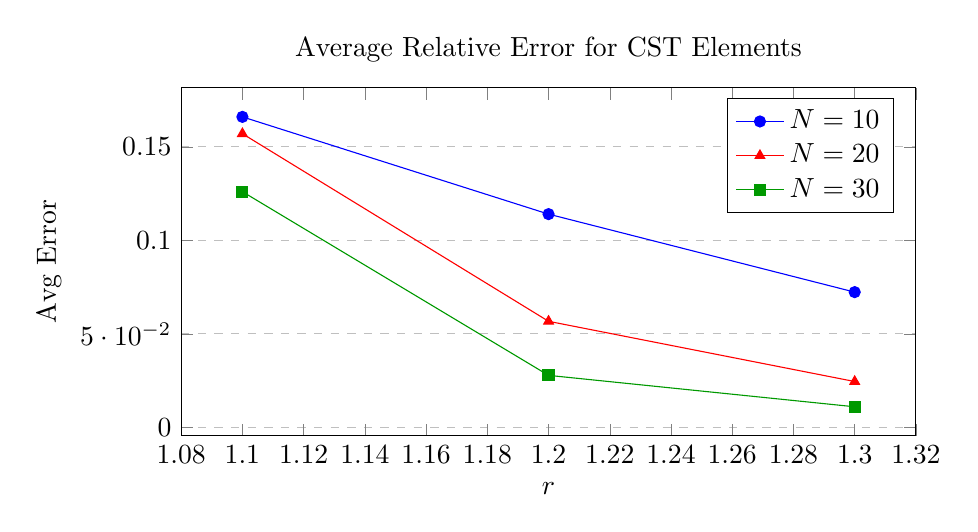
\begin{tikzpicture}
\begin{axis}[
    title={Average Relative Error for CST Elements},
    xlabel={$r$},
    ylabel={Avg Error},
    legend pos=north east,
    ymajorgrids=true,
    grid style=dashed,
    width=0.9\textwidth,
    height=6cm
]
\addplot[color=blue, mark=*] coordinates {
    (1.1, 0.166)
    (1.2, 0.114)
    (1.3, 0.0723)
};
\addlegendentry{$N = 10$}

\addplot[color=red, mark=triangle*] coordinates {
    (1.1, 0.157)
    (1.2, 0.0567)
    (1.3, 0.0245)
};
\addlegendentry{$N = 20$}

\addplot[color=green!60!black, mark=square*] coordinates {
    (1.1, 0.126)
    (1.2, 0.0278)
    (1.3, 0.0110)
};
\addlegendentry{$N = 30$}
\end{axis}
\end{tikzpicture}
\caption{Average relative error for CST elements varying $r$ and $N$.}
\label{fig:cst_avg_error_plot}
\end{figure}

In the case of CST elements, we observe that the average relative error decreases as the refinement parameter $r$ increases, indicating that finer meshes lead to more accurate solutions. However, the errors remain relatively high compared to LST elements.

\begin{figure}[H]
\centering
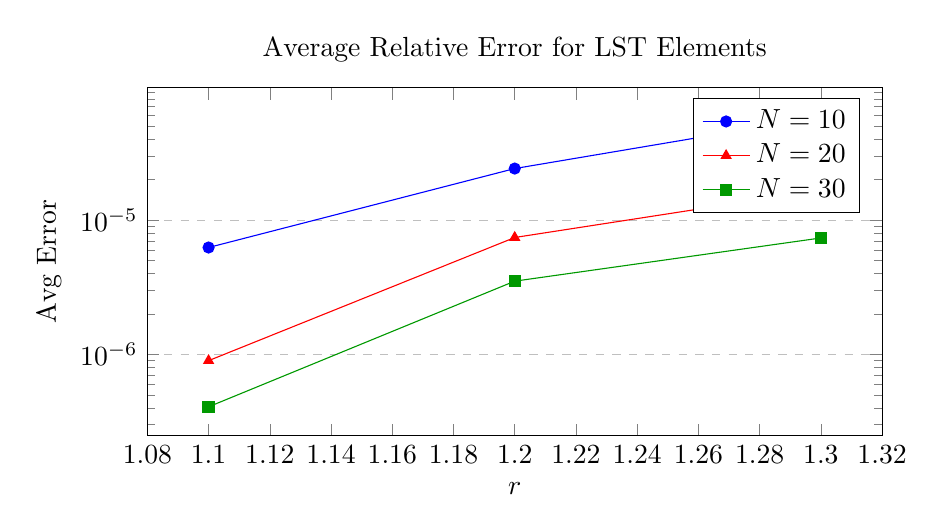
\begin{tikzpicture}
\begin{axis}[
    title={Average Relative Error for LST Elements},
    xlabel={$r$},
    ylabel={Avg Error},
    ymode=log,
    legend pos=north east,
    ymajorgrids=true,
    grid style=dashed,
    width=0.9\textwidth,
    height=6cm
]
\addplot[color=blue, mark=*] coordinates {
    (1.1, 6.25e-6)
    (1.2, 2.42e-5)
    (1.3, 5.87e-5)
};
\addlegendentry{$N = 10$}

\addplot[color=red, mark=triangle*] coordinates {
    (1.1, 8.98e-7)
    (1.2, 7.42e-6)
    (1.3, 1.67e-5)
};
\addlegendentry{$N = 20$}

\addplot[color=green!60!black, mark=square*] coordinates {
    (1.1, 4.07e-7)
    (1.2, 3.51e-6)
    (1.3, 7.36e-6)
};
\addlegendentry{$N = 30$}
\end{axis}
\end{tikzpicture}
\caption{Average relative error for LST elements varying $r$ and $N$ (log scale).}
\label{fig:lst_avg_error_plot}
\end{figure}

\vspace{0.3cm}
\noindent
As shown in LST Figure, the average relative error for LST elements increases with larger values of $r$, indicating that sharper gradients reduce accuracy. However, increasing $N$ consistently decreases the error, demonstrating the convergence of the method. The use of a logarithmic scale highlights the high precision of LST elements, with errors significantly lower than those of CST elements.



\newpage
\section{Conclusion}

This study implemented and evaluated the finite element solution of the two-dimensional Poisson equation using both linear (CST) and quadratic (LST) triangular elements on geometrically refined unstructured meshes. The use of the Method of Manufactured Solutions (MMS) enabled precise error quantification and verification of convergence behavior.

The results confirm that increasing the number of subdivisions $N$ consistently reduces the relative error for both element types. However, a significant performance difference was observed: LST elements yielded errors several orders of magnitude lower than CST elements for the same mesh resolution. This demonstrates the superior approximation capacity of quadratic elements.

While moderate geometric refinement ($r$) helped improve accuracy by concentrating nodes in regions of high gradient, excessive refinement (e.g., $r = 1.3$) slightly increased the error in some LST cases due to degradation in element shape quality. This highlights that higher-order elements, although more accurate, are also more sensitive to mesh distortion.

In summary, LST elements offer superior accuracy and convergence when mesh quality is preserved. Effective mesh design and appropriate refinement strategies are critical to fully exploit the advantages of higher-order finite elements in solving elliptic PDEs.

\end{document}